% English version of the refined Kauffman paper (hep-th style). Not a translation of paper/ja_v2.
% Structure (after the second round of review, 2026-11-10): definition -> index -> Hopf -> fundamental representation
% -> general N -> cables -> Sp -> cover -> multi-box obstructions -> open problems; computational details, closed strings,
% further structure of the fixed sector and the generated data are appendices.
% Claim grading: paper/claims.md (IDs in % [..] comments). Bibliography shared with ja_v2/refs.bib.
% Compile: cd docs/refined_kauffman/paper/en && TEXMFVAR=$TMPDIR/texmfvar lualatex main.tex && bibtex main && lualatex main.tex (twice)
\documentclass[11pt,a4paper]{article}
\usepackage[T1]{fontenc}
\usepackage{lmodern}
\usepackage{amsmath,amssymb,amsthm,bm}
\usepackage{booktabs,array,graphicx}
\usepackage{tikz}
\usetikzlibrary{positioning,decorations.pathreplacing}
\usepackage{youngtab}
\Yboxdim{5pt}
\DeclareRobustCommand{\yone}{\yng(1)}
\DeclareRobustCommand{\ytwo}{\yng(2)}
\DeclareRobustCommand{\yoneone}{\yng(1,1)}
\DeclareRobustCommand{\ythree}{\yng(3)}
\DeclareRobustCommand{\ytwoone}{\yng(2,1)}
\DeclareRobustCommand{\yoneoneone}{\yng(1,1,1)}
\usepackage[margin=25mm]{geometry}
\usepackage[backend=bibtex,style=alphabetic,maxalphanames=4,minalphanames=4,maxbibnames=10,doi=true,eprint=true]{biblatex}
\addbibresource{../ja_v2/refs.bib}
\usepackage[hidelinks,pdftitle={Refined crosscap invariants and the large N duality for colored Kauffman invariants},pdfauthor={Masaya Kameyama}]{hyperref}
\allowdisplaybreaks
\sloppy
\numberwithin{equation}{section}

\newtheorem{theorem}{Theorem}[section]
\newtheorem{proposition}[theorem]{Proposition}
\newtheorem{corollary}[theorem]{Corollary}
\newtheorem{conjecture}[theorem]{Conjecture}
\theoremstyle{definition}
\newtheorem{definition}[theorem]{Definition}
\newtheorem{hypothesis}[theorem]{Hypothesis}
\newtheorem{result}[theorem]{Result}
\theoremstyle{remark}
\newtheorem{remark}[theorem]{Remark}

\newcommand{\ba}{\bm{a}}
\newcommand{\bq}{\bm{q}}
\newcommand{\bt}{\bm{t}}
\newcommand{\tlam}{\tilde\lambda}
\newcommand{\ql}{q_\ell}
\newcommand{\qr}{q_r}
\newcommand{\Rred}{\mathcal{R}}
\newcommand{\SO}{\mathrm{SO}}
\newcommand{\U}{\mathrm{U}}
\newcommand{\Sp}{\mathrm{Sp}}
\newcommand{\GL}{\mathrm{GL}}
\newcommand{\cov}{\mathrm{cov}}
\newcommand{\Sym}{\mathrm{Sym}}
\newcommand{\Tr}{\mathrm{Tr}}
\DeclareMathOperator{\mirror}{mirror}
\newcommand{\open}{\emph{(open)}}
\newcommand{\Cab}[1]{\mathcal{C}_{#1}}        % algebraic cables of the trefoil
\newcommand{\Nfix}{\mathcal{N}}               % generating function of the fixed sector (brane 1, image 1)
\newcommand{\Bim}{\mathcal{B}}                 % brane--image sector of the cover
\newcommand{\Phifix}{\Phi}                     % index of the fixed sector, (1-t) f^cov restricted to it
\newcommand{\cK}{\mathsf{c}_K}                 % knot-dependent constant in the GL normalization

\title{Refined crosscap invariants and the large $N$ duality\\ for colored Kauffman invariants}
\author{Masaya Kameyama}
\date{November 10, 2026 (draft)}

\begin{document}
\maketitle

\begin{abstract}
We refine the large $N$ duality for the colored Kauffman invariant of $\SO(N)$ Chern--Simons theory \cite{Marino09} in the framework of the orientifold refined topological string \cite{AgSc12}. The refined crosscap invariant is defined as $g = f - \tfrac12 f^{\cov}$, where $f$ is the free energy of the $\SO(2N)$ refined Chern--Simons invariants with the dual Cauchy kernel of Koornwinder polynomials and $f^{\cov}$ that of the $\U(2N-1)$ cover in composite representations, both in a uniform normalization. From the M-theory index of the orientifold we derive the structure $g = \tfrac12 E/(1+t) + C$, with $E$ the signed sum over states invariant under the orientifold involution and $C$ the sum over frozen states, and the boundary factor $z_q^{n-1}(z_q^+)^n$ of $E$. Using DAHA-Jones polynomials of types $D_N$ and $GL_N$ at generic $t$, we compute $g$ at general $N$ for the trefoil up to four boxes, for $T(2,5)$, $T(2,7)$, $T(2,9)$ up to three boxes and, through the iterated DAHA-Jones polynomials of \cite{CD14}, for two algebraic cables of the trefoil. In every case the $N$-dependent poles cancel, the invariants are integer Laurent polynomials up to the factor $2(1+t)$ predicted by the index in even sectors, and the refined part is divisible by the universal factor $(\bt^2 - 1)(\ba^2 - \bq^2)$. For the fundamental representation of two-strand torus knots the $c = 1$ part has a $G$-expansion with aligned signs in each $\lambda^\beta$ block and the $c = 2$ part is $-(\ba^2 - \bq^2)(\bt^2 - 1)$ times a positive polynomial; this criterion fails for $T(3,4)$ and for the cables, where the $c = 1$ part is not $\sigma$-symmetric. Splitting the cover into brane and image, the brane--brane sector reproduces the refined LMOV invariants of \cite{KN17} and the brane--image sector is identified as a space of states for two-strand torus knots. The refined $\Sp(2N)$ invariants of \cite{AM22} satisfy $g^{\Sp}(\ba) = -g^{\SO}(-\ba)$ in the fundamental representation. For higher representations the $c = 1$ part is not $\sigma$-symmetric and the signs do not align; the obstruction is localized in the multiplet structure of the frozen states.
\end{abstract}


\tableofcontents

\section{Introduction}\label{sec:intro}

\subsection{Background}
The colored HOMFLY-PT invariants of $\U(N)$ Chern--Simons theory are dual, at large $N$, to open topological strings on the resolved conifold, and the Ooguri--Vafa reformulation writes them in terms of integer BPS invariants (the LMOV invariants, after Labastida, Mari\~no, Ooguri and Vafa). For $\SO(N)$ and $\Sp(N)$ the dual theory is the topological string on an orientifold of the Calabi--Yau, as proposed in \cite{SV00}. It was conjectured in \cite{Marino09}, and verified there in many examples, that the colored Kauffman invariant of $\SO(N)$ minus one half of the $\U(N)$ invariant in composite representations is expressed through integer BPS invariants with crosscap number $c = 1, 2$ (see also \cite{BFM04,BFM05,NRZ13}). On the homological side, a Kauffman homology and superpolynomials for two-strand torus knots were proposed in \cite{GW05}, and the relation between $\SO$/$\Sp$ invariants, composite representations and BPS states was studied in \cite{GS11}.

Refined Chern--Simons theory was formulated in \cite{AgSh11}, and it was shown in \cite{KN17} that the $\U(N)$ refined Chern--Simons invariants produce refined BPS invariants on the resolved conifold which, for torus knots, are positive integers (refined large $N$ duality). In \cite{AgSc12} the refined topological string on an orientifold was defined as an M-theory index, the $\SO(2N)$ refined Chern--Simons invariants were computed, and the closed string free energy at large $N$ was shown to satisfy the integrality of second quantization. The closed $\SO$ and $\Sp$ free energies were organized with multiple sine functions in \cite{AM22}. For open strings, i.e.\ for knots, neither a formula extracting refined crosscap BPS invariants nor a test of their integrality has been available.

\subsection{Questions}
We address the following questions.
\begin{enumerate}
\item How does one extract a refined crosscap invariant from the $\SO(2N)$ refined Chern--Simons invariants?
\item Does it have an integral BPS expansion? If so, what structure does it have (universal factor, structure in the winding number $d$, boundary factors)?
\item Is positivity visible after refinement, i.e., do the coefficients align in sign in a suitable multiplet basis? Where does it hold and where does it break?
\item How is it related to the $\U(2N-1)$ cover, and how much of the crosscap structure is determined by the cover?
\item What remains open for higher representations?
\end{enumerate}
Question 1 is answered by the definition in \S\ref{sec:setup}. Question 2 is answered by the all-$d$ structure and the boundary factors (\S\ref{sec:index}) and by the integrality and the universal factor at general $N$ (\S\ref{sec:generalN}), including iterated torus knots. Question 3 is answered by the criterion in the fundamental representation (\S\ref{sec:torus}), by the signs of the brane--brane and brane--image sectors of the cover (\S\ref{sec:cover}) and by the multi-box crosscap signs (\S\ref{sec:positivity}): positivity holds in the fundamental representation of two-strand torus knots and on the cover side, and fails for the multi-box crosscap part and for the fundamental representation of knots that are not two-strand torus knots. Question 4 is addressed in \S\ref{sec:cover}, and question 5 in \S\ref{sec:positivity} and \S\ref{sec:discussion}.

\subsection{Main results}
Table~\ref{tab:summary} summarizes the range of verification.
\begin{itemize}
\item \textbf{Definition (\S\ref{sec:setup}).} A naive refinement of the bosonic kernel of \cite{Marino09} fails already for the unknot with two boxes: poles in $U = t^N$ do not cancel. With the dual Cauchy kernel of Koornwinder polynomials (the dual Cauchy identity of \cite{Mimachi01}) the product formula for the unknot is automatic. We take the uniform normalization in which the $\U(n)$ invariants are invariant under determinant shifts and charge conjugation, and the reformulation matrix $M(q^{-1})$ of \cite{Marino09}. The refined crosscap invariant is $g = f - \tfrac12 f^{\cov}$ (Definition \ref{def:crosscap}); $f$ is computed from the $\SO(2N)$ refined invariants and $f^{\cov}$ from the A-type invariants of the cover (ordinary and composite representations), separately and order by order in the number of boxes.
\item \textbf{All-$d$ structure (\S\ref{sec:index}).} The M-theory index of the orientifold gives $g = \tfrac12 E/(1+t) + C$ (Proposition \ref{prop:alld}), where $E$ is the signed sum over states invariant under the involution $\tilde I$ and $C$ the sum over frozen states; $E$ appears only in sectors with equal numbers of brane and image boxes. The same identity is the $\SO(2N)$ version of the trace representation of the Chern--Simons partition function of \cite{Witten11} (Remark \ref{rem:trace}). From the action of $\tilde I$ on boundary zero modes we derive the boundary factor $z_q^{n-1}(z_q^+)^n$ of $E$ (Proposition \ref{prop:boundary}) and verify it for the Hopf link and the framed unknot; for knots it is consistent with all computations. For closed strings the product formula of the $\SO(2N)$ partition function agrees with \cite{AgSc12}, and the ``Klein bottle'' term of \cite{AM22} is a rearrangement of this decomposition (Proposition \ref{prop:AM}). The separation of $E$ and $C$ is not determined by the index (Proposition \ref{prop:EC}).
\item \textbf{Unknot and Hopf link (\S\ref{sec:hopf}).} Integrality holds, the K\"ahler variable is shifted to $\tlam = \lambda(q/t)^{1/2}$, and $E_{22}$, $E_{24}$ are determined uniquely under a hypothesis on the numbers of states (Hypothesis \ref{hyp:QP}) and Hypothesis \ref{hyp:E2}.
\item \textbf{The criterion in the fundamental representation (\S\ref{sec:torus}).} For $T(2,2m+1)$, $m \le 5$, the $c = 1$ part has a $G$-expansion and the $c = 2$ part a closed form, with signs aligned in each $\lambda^\beta$ block. We state this as a criterion (Conjecture \ref{conj:criterion}). The criterion is specific to two-strand torus knots: for $T(3,4)$ and for algebraic cables the $c = 1$ part is not $\sigma$-symmetric, and for the cables the refined part of the $c = 2$ part has mixed signs (\S\ref{sec:cable}).
\item \textbf{Integrality and the universal factor at general $N$ (\S\ref{sec:generalN}).} Computing DAHA-Jones polynomials at generic $t$, we obtain the refined $\SO(2N)$ invariants at general $N$ for the trefoil with two to four boxes, $T(2,5)$ with two and three boxes, and $T(2,7)$, $T(2,9)$ with three boxes. The crosscap parts are integer Laurent polynomials in odd sectors, and $2(1+t)g_R$ is an integer Laurent polynomial in even sectors, the $(1+t)$ poles sitting exactly where Proposition \ref{prop:alld} predicts. The refined part is divisible by the universal factor $(\bt^2 - 1)(\ba^2 - \bq^2)$ (Conjecture \ref{conj:structure}).
\item \textbf{Algebraic cables (\S\ref{sec:cable}).} Taking the $D_N$ value of the iterated DAHA-Jones polynomial of \cite{CD14} as the definition, we obtain the fundamental representation and the two-box invariants of the $(2,13)$-cable of the trefoil and the fundamental representation of the $(2,15)$-cable at general $N$. Integrality, the position of the $(1+t)$ poles and the universal factor hold as for torus knots.
\item \textbf{Refined $\Sp(2N)$ (\S\ref{sec:sp}).} Implementing the $C_N$ DAHA, we obtain the refined $\Sp(2N)$ invariants of \cite{AM22} for the trefoil and $T(2,5)$ in the fundamental representation and for the trefoil with two boxes at general $N$. In the fundamental representation $g^{\Sp}(\ba) = -g^{\SO}(-\ba)$; with two boxes $W_R^{\Sp}(\ba) = (-1)^{|R|}W_R^{\SO}(-\ba)$, and the difference of the crosscap parts is the closed form $\pm\psi^2[\Delta]$. These are refined versions of the classical correspondence $\Sp(N) = \SO(-N)$ \cite{Cvitanovic08,MV10}.
\item \textbf{Structure of the cover (\S\ref{sec:cover}).} Splitting the cover into brane and image, the brane--brane sector coincides coefficient by coefficient with the $\U(N_A)$ refined LMOV invariants of \cite{KN17}. After removing boundary factors, the brane--image sector of two-strand torus knots is identified as a space of states built from $\Sym^k V$, $S \otimes S$ and universal corrections $F_{j'}$ (Result \ref{cr:principle}, Conjecture \ref{conj:closedform}); the generating function written with the rows of the fundamental and adjoint representations (Proposition \ref{prop:rows}) holds for fourteen torus knots. From this identification, fitted on $T(2,3)$--$T(2,9)$, $E$ is predicted for $T(2,11)$--$T(2,15)$ and reads as a signed partial sum of numbers of states.
\item \textbf{Multi-box status (\S\ref{sec:positivity}).} For higher representations the $c = 1$ part of the crosscap invariant is not $\sigma$-symmetric, has no $G$-expansion, and its signs do not align. The $\sigma$-asymmetry splits into a part that is already present in the unrefined theory, due to the parity rule relating $c$ to the power of $\lambda$ (in hatted invariants $\beta \equiv |R| - 1$), and a part specific to refinement, the $\sigma$-odd part divisible by $(\bt^2 - 1)(\ql - \ql^{-1})$. Since the cover is well behaved, the obstruction is localized in the multiplet structure of the frozen states.
\end{itemize}

\begin{table}[htbp]
\centering
\small
\caption{Range of verification. ``Integer'' means an integer Laurent polynomial; for even $|R|$ the crosscap part $g_R$ has the denominator $2(1+t)$ predicted by Proposition~\ref{prop:alld}, and ``$2(1+t)g_R$'' means that $2(1+t)g_R$ is integer while $g_{\ytwo} + g_{\yoneone}$ is integer as well. ``Universal factor'' is the divisibility of \S\ref{sec:universal}. ``Signs'': number of $\ba$-blocks of the quotient by the universal factor with aligned signs / total number of blocks; ``criterion'' refers to Conjecture~\ref{conj:criterion}; ``switching block'' is the block $k = 2m$ at which the universal series turns into the knot part (\S\ref{sec:split}).}\label{tab:summary}
\setlength{\tabcolsep}{4pt}
\begin{tabular}{p{4.3cm}p{2.7cm}p{2.5cm}p{5.0cm}}
\toprule
Object & Integer & Universal factor & Signs \\
\midrule
\addlinespace
Unknot, Hopf link ($a, b \le 4$) & yes & yes (10 components of $\hat C_{R,S}$) & $\hat g_{R,\yone}$ aligned; refined part of $\hat C_{R,S}$: 8/10 \\
\addlinespace
$T(2,2m+1)$, fundamental ($m \le 5$) & yes & yes & criterion holds \\
\addlinespace
$T(2,2m+1)$, fixed $N$ ($N = 2, 3$, $|R| \le 3$, $m \le 3$) & hatted invariants integer in all power-sum directions & --- & not decidable at fixed $N$ \\
\addlinespace
Trefoil, two boxes (large $N$) & $2(1+t)g_R$ & yes & 5/10 \\
\addlinespace
$T(2,5)$, two boxes & $2(1+t)g_R$ & yes & 6/18 \\
\addlinespace
Trefoil, three boxes & yes (no $(1+t)$ pole; hatted integer) & yes & 2/15, 3/14, 2/13 \\
\addlinespace
$T(2,5)$, $T(2,7)$, $T(2,9)$, three boxes & yes (no $(1+t)$ pole) & yes & 1/23--1/25, 1/33--1/35, 1/43--1/45 \\
\addlinespace
Trefoil, four boxes & $2(1+t)g_R$ ($(1+t)$ only in $p_4$, $p_2^2$) & yes & 0--2/18--22 \\
\addlinespace
$T(3,4)$, fundamental & yes & yes & criterion fails: $c = 1$ not $\sigma$-symmetric; $c = 2$ aligned per block; quotient of $g$: 4/4 \\
\addlinespace
Algebraic cables $\Cab{13}$, $\Cab{15}$, fundamental & yes & yes & criterion fails: $c = 1$ not $\sigma$-symmetric, refined part of $c = 2$ mixed; quotient of $g$: 6/9, 8/11 \\
\addlinespace
$\Cab{13}$, two boxes & $2(1+t)g_R$ & yes & 30/50 \\
\addlinespace
Cover, brane--brane (trefoil, $T(2,5)$, $|R| \le 2$) & yes (equals \cite{KN17}) & --- & all blocks aligned \\
\addlinespace
Cover, brane--image ($\Nfix$ with boundary factors removed; $T(2,3)$, $T(2,5)$, $T(2,7)$) & yes & --- & trefoil: all blocks aligned; $T(2,5)$, $T(2,7)$: aligned except the switching block \\
\addlinespace
Refined $\Sp(2N)$: $T(2,3)$, $T(2,5)$ fundamental; trefoil two boxes & yes (same structure as $\SO$) & --- & $g^{\Sp}(\ba) = -g^{\SO}(-\ba)$; $W_R$: $(-1)^{|R|}$ \\
\bottomrule
\end{tabular}
\end{table}

\subsection{Classification of claims and organization}
Statements are graded as follows. Propositions and corollaries are derived analytically, possibly under an explicitly stated hypothesis. A \emph{Result} is a statement verified by computer, with the range of verification stated. Conjectures are closed forms or structures suggested by computation beyond the verified range. Hypotheses are rules that could not be taken directly from the literature; we say which verification supports them. Definitions and remarks have their usual meaning. In the discussion, [derivation] and [computation] mark the two kinds of evidence, and \open\ marks an open point. Computational methods are described in Appendix \ref{app:code}. Abbreviations: DAHA (double affine Hecke algebra), LMOV (Labastida--Mari\~no--Ooguri--Vafa), TN (Taub--NUT), CoHA (cohomological Hall algebra).

\S\ref{sec:setup} fixes variables, kernel and normalization and defines the refined crosscap invariant. \S\ref{sec:index} derives the all-$d$ structure and the boundary factors from the orientifold index. \S\ref{sec:hopf} treats the unknot and the Hopf link, \S\ref{sec:torus} the criterion in the fundamental representation of torus knots, \S\ref{sec:generalN} the integrality and the universal factor at general $N$ for higher representations and for algebraic cables, and \S\ref{sec:sp} the refined $\Sp(2N)$ invariants. \S\ref{sec:cover} splits the cover into brane and image, \S\ref{sec:positivity} summarizes the status and obstructions for multi-box crosscap invariants, and \S\ref{sec:discussion} lists open problems.

\section{Refined crosscap invariants}\label{sec:setup}

\subsection{Variables}\label{sec:variables}
\begin{center}
\small
\begin{tabular}{>{$}l<{$}p{9.5cm}}
\toprule
\text{symbol} & meaning \\
\midrule
q,\ t & variables of refined Chern--Simons theory (as in \cite{KN17}); half-integer powers $q^{1/2}, t^{1/2}$ are written as such \\
\lambda = t^{N - 1/2} & Kauffman variable ($\lambda$ of \cite{NRZ13}, $\nu$ of \cite{Marino09}); $N$ is the rank of $D_N$ and $t^N = \lambda t^{1/2}$. At $t = q$ it is the $\lambda = q_{\mathrm{NRZ}}^{2N-1}$ of \cite{NRZ13} ($q_{\mathrm{NRZ}} = q^{1/2}$); at large $N$ it is treated as a formal variable \\
\tlam = \lambda\, \qr & shifted Kauffman variable ($-\ba\bt$ in bold variables) \\
a = \lambda^2 = t^{N_A},\ N_A = 2N - 1 & K\"ahler variable of the cover $\U(N_A)$ ($a = t^{N_A}$ of \cite{KN17}) \\
(\bq, \bt, \ba) = (t^{1/2}, -\qr, \lambda) & bold variables; $\bq, \bt$ as in \cite{KN17} ($q^{1/2} = -\bq\bt$, $t^{1/2} = \bq$), $\ba = \lambda$ as in \cite{AgSc12}. The $\ba$ of the cover in \cite{KN17} is defined by $a = -\ba_{\mathrm{KN}}^2\bt$, so $\ba_{\mathrm{KN}} = \ba\,(t/q)^{1/4}$ \\
\ql = (qt)^{1/2},\ \qr = (q/t)^{1/2} & $q_\ell, q_r$ of \cite{KN17} ($q = \ql\qr$, $t = \ql/\qr$); $w := \qr$ is the notation of \cite{AM22} \\
z_q = q^{1/2} - q^{-1/2},\ z_t = t^{1/2} - t^{-1/2} & $z_q^+ = q^{1/2} + q^{-1/2}$ \\
G = z_q z_t = \ql + \ql^{-1} - \qr - \qr^{-1} & variable of the $G$-expansion; $(\bq\bt - \bq^{-1}\bt^{-1})(\bq - \bq^{-1}) = -G$ in \cite{KN17} \\
\sigma\colon q \mapsto t^{-1},\ t \mapsto q^{-1} & $\ql \mapsto \ql^{-1}$ with $\qr$ and $\lambda$ fixed; $G$ is invariant \\
\text{mirror} & $\lambda \mapsto \lambda^{-1}$, $q \mapsto q^{-1}$, $t \mapsto t^{-1}$ (the mirror image of the knot) \\
\delta & the Seifert genus of the knot: $\delta = m$ for $T(2,2m+1)$, $(r-1)(s-1)/2$ for $T(r,s)$; for thin knots it equals the $\delta$-degree $\deg_{\ba} + \tfrac12\deg_{\bq} - \deg_{\bt}$ of the superpolynomial \\
\bottomrule
\end{tabular}
\end{center}
In the unrefined limit $t = q$ the variables of \cite{Marino09} are $t_M = q^{1/2}$ and $z = z_q$, and the $q_{\mathrm{NRZ}}$ of the Kauffman polynomial $F_R(K; \lambda, q_{\mathrm{NRZ}})$ of \cite{NRZ13} is also $q^{1/2}$. Young diagrams are written as $R, \mu, \nu$ (never $\lambda$); in displayed formulas we draw them, e.g.\ $g_{\ytwo}$, and in the text we write $[2]$, $(2)$ for the same diagram. Composite representations of $\U(N_A)$ are written $(\alpha;\bar\beta)$; the adjoint is $(1;\bar1)$.

\subsection{Refined \texorpdfstring{$\SO(2N)$}{SO(2N)} invariants}
In the $\SO(2N)$ refined Chern--Simons theory of \cite{AgSc12}, the Wilson loop in a representation $R$ is given by a Macdonald polynomial of type $D_N$.
% [S1]
\begin{result}\label{cr:dim}
The refined unknot $\dim_R$ of \cite{AgSc12} equals the principal specialization $x = (1, t, \dots, t^{N-1})$ of the Koornwinder polynomial \cite{Koornwinder92} $K_R(x; q, t; 1, -1, q^{1/2}, -q^{1/2})$ for six representations with $|R| \le 3$ (checked against the evaluation formulas of \cite{vD96,Sahi99} and against polynomials constructed by the $q$-difference operator for $N = 2, 3$).
$\dim_R$ is not a Laurent polynomial in $t^N$: for instance, for the representation $[2]$ it has the denominator $(1 - qt^{N-1})$ and for $[1,1]$ the denominator $(1 - qt^{2N-3})$; both cancel at $t = q$.
\end{result}

% [S2]
\begin{remark}[failure of the naive refinement]
If the construction of \cite{Marino09} is refined as it stands (bosonic Cauchy kernel, the factor $\tfrac12$, the sum over odd $d$), the poles in $U = t^N$ fail to cancel already for the two-box unknot. The composite $([1],[1])$ contributes only in the $p_1^2$ direction, whereas the poles of the $D_N$ representations $[2]$ and $[1,1]$ sit at different places ($t^N = t/q$ and $t^{2N} = t^3/q$). None of five choices of weights and three choices of basis removes the mismatch.
\end{remark}

\subsection{Dual Cauchy kernel and generating function}\label{sec:kernel}
% [S3]
In the dual Cauchy identity for Koornwinder polynomials \cite{Mimachi01},
\begin{equation}\label{eq:mimachi}
\sum_{\mu \subseteq m^n} (-1)^{|\mu|} K_{m^n - \mu}(x; q, t)\, K_{\mu'}(y; t, q) = \prod_{i, j} x_i^{-1}(1 - x_i y_j)(1 - x_i y_j^{-1}),
\end{equation}
the holonomy side carries the $D_n$-type parameters $(\pm1, \pm q^{1/2})$ of \cite{AgSc12} and the probe side the parameters $(\pm 1, \pm t'^{1/2})$ for $(q', t') = (t, q)$. We checked the identity for $(n, m) = (1,1), (2,1), (1,2), (2,2), (2,3), (3,2)$.
We read this identity as the Ooguri--Vafa kernel of the refined orientifold and set, for probe variables $Y = (y_1, y_2, \dots)$,
\begin{equation}\label{eq:Z}
\tilde Z(Y) = \Bigl\langle \prod_{\alpha, i} (1 - y_\alpha x_i)(1 - y_\alpha x_i^{-1}) \Bigr\rangle_{\SO(2N)},\qquad
\log \tilde Z = \sum_{d \ge 1} \frac1d \sum_R f_R(q^d, t^d, \lambda^d)\, s_R(Y^d).
\end{equation}
Here $\langle F(x)\rangle_{\SO(2N)}$ is the linear map that expands a class function $F$ of the holonomy eigenvalues $x = (x_1, \dots, x_N)$ in Koornwinder polynomials $K_\mu(x; q, t; 1, -1, q^{1/2}, -q^{1/2})$ and replaces each term by the refined Chern--Simons knot invariant $W_\mu(K)$ (normalized as in \S\ref{sec:uniform}): $F = \sum_\mu c_\mu K_\mu(x)$ gives $\langle F\rangle := \sum_\mu c_\mu W_\mu(K)$. In the unrefined theory this is the path-integral expectation value of the Wilson loop, in which $x$ is integrated out. The sum in \eqref{eq:Z} runs over all $d$ (``all-$d$''), not only over odd $d$ as in \cite{Marino09}.

Since $(1 - x_iy_j^{-1}) = -x_iy_j^{-1}(1 - y_jx_i^{-1})$, the right-hand side of \eqref{eq:mimachi} with $n = N$ equals $(-1)^{Nm}(\prod_j y_j)^{-N}\prod_{i,j}(1 - y_jx_i)(1 - y_jx_i^{-1})$. Reading the identity with $m$ probes on the $y$ side and $N$ holonomies on the $x$ side, the kernel of \eqref{eq:Z} is therefore
\begin{equation}\label{eq:Zexpand}
\begin{aligned}
\tilde Z(Y) &= \sum_{\mu \subseteq m^N} (-1)^{|\mu| + Nm}\, W_\mu(K)\, \hat K_{\mu'}(Y; t, q; T = t^N),\\
\hat K_{\mu'}(Y; t, q; T) &:= \Bigl(\prod_\alpha y_\alpha\Bigr)^N K_{N^m - \mu'}(Y; t, q; 1, -1, q^{1/2}, -q^{1/2}).
\end{aligned}
\end{equation}
The expansion runs over Koornwinder polynomials of type $(t, q)$ on the probe side; the complement in the rectangle $N^m$ multiplied by $(\prod y)^N$ is a virtual Koornwinder polynomial \cite{Rains05,RW21}, which depends on $N$ only through $T = t^N = U$. The kernel in \eqref{eq:Z} has no prefactor, so setting $y_{m+1} = 0$ reduces the $(m+1)$-probe kernel to the $m$-probe one; hence $\log\tilde Z$ is a well-defined symmetric function of $Y$ and $f_R$ does not depend on the number of probes once $m \ge \ell(R)$. The invariant $f_R$ is defined by expanding $\log\tilde Z$ in Schur functions $s_R(Y)$ and applying M\"obius inversion in $d$. In the actual computation (Appendix \ref{app:code}) the kernel $\prod_{\alpha,i}(1 - y_\alpha x_i)(1 - y_\alpha x_i^{-1}) = \exp(-\sum_d p_d(Y)S_d(x)/d)$, $S_d(x) = \sum_i(x_i^d + x_i^{-d})$, is expanded in $K_\mu(x)$ by evaluating at the points $x = t^\rho q^\nu$, where $S_d(t^\rho q^\nu)$ is a rational function of $U$; this is why $U$ can be treated as a formal variable, independently of the closed form of \S\ref{sec:virtual}. The sign $(-1)^{|\mu|}$ is the hallmark of a fermionic kernel. For the unknot $W_\mu = P_\mu(t^\rho)$ and \eqref{eq:Zexpand} reduces to the dual Cauchy identity evaluated at $x = t^\rho$, which is a product (\S\ref{sec:unknot}).

For the cover $\U(N_A)$ we define $f^{\cov}_R$ with the same kernel $\prod_i(1 - y_\alpha x_i)(1 - y_\alpha x_i^{-1})$. Since both $x$ and $x^{-1}$ enter, the expansion basis consists of Macdonald characters of composite representations $(\alpha; \bar\beta)$, and $\langle P_\alpha(x) P_\beta(x^{-1})\rangle$ is evaluated by decomposing into composite values and contraction terms (\S\ref{sec:generalN}).
The part of the kernel with $|Y| \le 2$ is expressed through ordinary representations of $\U(N_A)$ and the adjoint composite $(1;\bar1)$; at degree three the composites $(2;\bar1)$ and $(1,1;\bar1)$ appear as well.

\begin{definition}[refined crosscap invariant]\label{def:crosscap}
In the all-$d$ definition \eqref{eq:Z} we set $g_R = f_R - \tfrac12 f^{\cov}_R$.
The hatted invariant is $\hat g = M(q^{-1})^{-1} g$, where $M_{RS} = \sum_\mu \chi_R(\mu)\chi_S(\mu) z_\mu^{-1}\prod_i (t_M^{\mu_i} - t_M^{-\mu_i})/(t_M - t_M^{-1})$ with $t_M = q^{1/2}$ is the matrix $M$ of \cite{Marino09}, which equals $M(x)$ of \cite{KN17} at $x = q^{-1}$.
\end{definition}

% [S8]
\begin{remark}
With $M(t)$ or $M(t^{-1})$ in place of $M(q^{-1})$ the Hopf link invariants are not Laurent polynomials; $M(q)$ exchanges $R \leftrightarrow R^T$.
The two formulations of \cite{KN17} (the $q$-side with the Macdonald Cauchy kernel and $M(t)$, the $t$-side with the dual Cauchy kernel and $M(q^{-1})$) give the same hatted invariants with two boxes (\S\ref{sec:generalN}).
\end{remark}

\subsection{Computational scheme}\label{sec:procedure}
The invariant $g_R$ of Definition \ref{def:crosscap} is computed in three steps. $f_R$ and $f^{\cov}_R$ are obtained separately, order by order in the number of boxes, and $g_R$ is their difference.
\begin{center}
\small
\begin{tabular}{lp{6.6cm}p{5.4cm}}
\toprule
quantity & input & computation \\
\midrule
$f_R$ & $\SO(2N)$ refined Chern--Simons invariants $W^{\SO}_\mu$, $|\mu| \le |R|$, type $D_N$ & expand $\log$ of the dual Cauchy kernel \eqref{eq:Z} in Schur functions and apply M\"obius inversion \\
$f^{\cov}_R$ & A-type invariants of the cover $\U(N_A)$: ordinary representations $W_\alpha$, the composite $(1;\bar 1)$ (adjoint), and for three boxes $(2;\bar 1), (1,1;\bar 1)$ with contraction terms & same kernel, expanded in composite Macdonald characters \\
$g_R$ & the two above & $f_R - \tfrac12 f^{\cov}_R$; hatted with $M(q^{-1})^{-1}$ \\
\bottomrule
\end{tabular}
\end{center}
$f_R$ closes on the $\SO$ side, and $f^{\cov}_R$ contains no $\SO$ data. That the cover is given by A-type refined invariants is a hypothesis---the refined version of the construction of \cite{Marino09}; for the fundamental representation it is stated as Hypothesis~\ref{hyp:hg}. It is supported by the fact that the cancellation of $N$-dependent poles after the subtraction fixes the framing monomial uniquely (Result~\ref{cr:uniform} and Result~\ref{cr:monomial}) and by the integrality of $g_R$ (\S\ref{sec:generalN}).
Writing the cover with two sets of probes, brane ($Y$) and image ($Y'$), $f^{\cov}$ splits into a brane--brane part (the invariant of \cite{KN17} itself) and a brane--image part (the connected part of the composites), see \S\ref{sec:cover}.

\subsection{Uniform normalization}\label{sec:uniform}
The input $\U(n)$ refined invariants, normalized by conditions (N1) and (N2) of \cite{KN17}, change by powers of $(q/t)$ under determinant shifts and charge conjugation. With $\delta$ the Seifert genus (\S\ref{sec:variables}) we set
\begin{equation}\label{eq:uniform}
W_R = (t/q)^{\delta |R|/2}\, \Rred_R\, P_R(t^\rho),
\end{equation}
where $\Rred_R$ is the reduced invariant (the refined invariant divided by that of the unknot; in \S\ref{sec:generalN} it is computed from DAHA-Jones polynomials) and $P_R(t^\rho)$ the Macdonald dimension.

% [S5][S6]
\begin{result}\label{cr:uniform}
For the normalization \eqref{eq:uniform} the following hold.
\begin{enumerate}
\item $W$ is exactly invariant under the determinant shift $R \to R + 1^n$ and under charge conjugation. Checked for 16 pairs for the trefoil ($\U(2)$--$\U(5)$), 13 pairs each for $T(2,5)$ and $T(2,7)$, and seven double twist knots.
\item At fixed $N$ ($N = 2, 3$, $|R| \le 3$), fixing the framing monomial by requiring the cancellation of $N$-dependent poles and the value $1$ at $t = q$ gives the monomial $1$ on both the $\SO$ side and the cover side ($T(2,3), T(2,5), T(2,7)$). Within the family $(t/q)^{\beta/2}$ the exponent $\beta$ is unique.
\item The DAHA-Jones polynomials (vertical framing) agree up to powers of the framing eigenvalue (\S\ref{sec:generalN}).
\item At $t = q$ this is the standard framing of \cite{Marino09}.
\end{enumerate}
\end{result}

% [S7]
\begin{hypothesis}\label{hyp:framing}
The uniform normalization \eqref{eq:uniform} is the normalization at framing zero.
\end{hypothesis}
We use this normalization on both sides throughout.

\subsection{The unknot}\label{sec:unknot}
% [H1]
\begin{proposition}\label{prop:unknot}
For the unknot, $f_{10} = (1 - t^N)(t^N + t)/(t^N(t-1))$ and $f_{a0} = 0$ for $a \ge 2$ (the first index counts probes on the knot, the second on a second component, cf.\ \S\ref{sec:hopf}). In terms of $\lambda$,
\[
f_{10} = -1 - \frac{\lambda - \lambda^{-1}}{t^{1/2} - t^{-1/2}},
\]
the sum of the unknot of \cite{Marino09}, $(\lambda - \lambda^{-1})/z$, and the crosscap term $-1$. In our conventions $g_{\yone}$ is minus the mirror of the crosscap invariant of \cite{Marino09} (Result \ref{cr:marino}), so $-1$ corresponds to the value $g_{\yone} = 1$ of \cite{Marino09} for the unknot. The product formula is $\prod_j (y_j^{\pm}; t)_\infty / (U y_j^{\pm}; t)_\infty$; neither the factor $\tfrac12$ nor the restriction to odd $d$ is needed.
\end{proposition}
\begin{proof}
The expectation value of the dual Cauchy kernel is $\prod_j\prod_{k=1}^{N} t^{-(N-k)}(1 - t^{N-k}y_j^{\pm})$; take the logarithm.
\end{proof}

\section{The orientifold index and the all-$d$ structure}\label{sec:index}

\subsection{Setup}\label{sec:index-setup}
Following \S3 of \cite{AgSc12}, M-theory on $\mathcal{X} \times \mathrm{TN} \times S^1$, with $\mathcal X$ the resolved conifold, is twisted by $(q, t)$. The orientifold action $\tilde I$ is the composition of an antiholomorphic involution $I$ of $\mathcal X$ with $z_2 \to -z_2$ in spacetime.
The probe of a knot $K$ is an M5-brane extended along the $z_2$ plane (a $t$-brane: the open-string denominator is $1/(1-t)$). On the cover there are two of them, $L_K$ and its image $I(L_K)$; see Figure \ref{fig:orientifold}.
The space of one-particle states on the cover is $H_1 = H_{\mathrm{int}} \otimes F_{z_2}$, where $F_{z_2}$ consists of the modes $t^l$, $l \ge 0$, in the $z_2$ direction, on which $\tilde I$ acts by $(-1)^l$. A \emph{sector} of the generating function is labelled by the numbers of boxes (total windings) on $L_K$ and on $I(L_K)$; a sector is \emph{fixed} when $\tilde I$ maps it to itself, i.e., when the two numbers are equal. States that exist only in the quotient, frozen at $z_2 = 0$ and wrapped on non-orientable surfaces, are called \emph{frozen states}.

\begin{figure}[htbp]
\centering
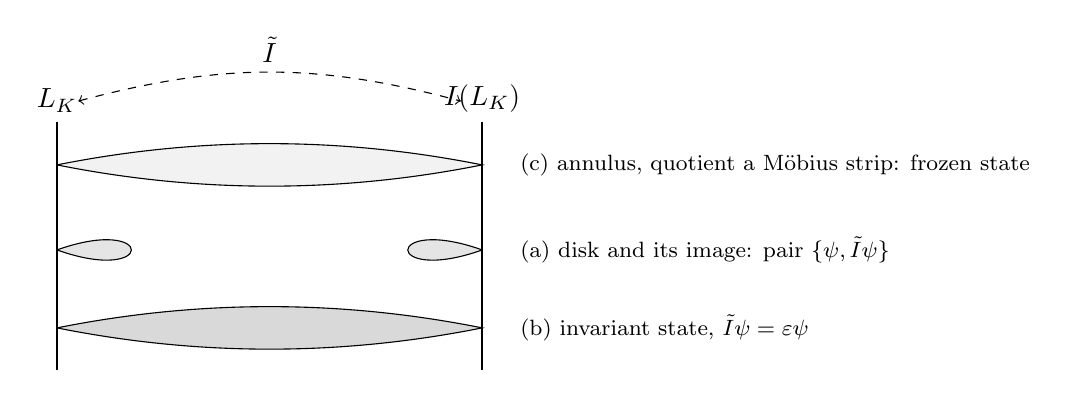
\begin{tikzpicture}[scale=0.9]
\draw[thick] (0,-0.3) -- (0,3.2) node[above] {$L_K$};
\draw[thick] (6,-0.3) -- (6,3.2) node[above] {$I(L_K)$};
\draw[<->,dashed] (0.3,3.5) to[bend left=15] node[midway,above] {$\tilde I$} (5.7,3.5);
% annulus between L and I(L): its quotient is a Moebius strip (frozen state)
\draw[fill=gray!10] (0,2.6) .. controls (2,3.0) and (4,3.0) .. (6,2.6) .. controls (4,2.2) and (2,2.2) .. (0,2.6);
\node[right] at (6.4,2.6) {\footnotesize (c) annulus, quotient a M\"obius strip: frozen state};
% pair: a disk on L_K and its image
\draw[fill=gray!20] (0,1.4) .. controls (1.4,1.9) and (1.4,0.9) .. (0,1.4);
\draw[fill=gray!20] (6,1.4) .. controls (4.6,1.9) and (4.6,0.9) .. (6,1.4);
\node[right] at (6.4,1.4) {\footnotesize (a) disk and its image: pair $\{\psi, \tilde I\psi\}$};
% invariant state: symmetric curve ending on both
\draw[fill=gray!30] (0,0.3) .. controls (2,-0.1) and (4,-0.1) .. (6,0.3) .. controls (4,0.7) and (2,0.7) .. (0,0.3);
\node[right] at (6.4,0.3) {\footnotesize (b) invariant state, $\tilde I\psi = \varepsilon\psi$};
\end{tikzpicture}
\caption{The cover with the brane $L_K$ and its image $I(L_K)$, and the three classes of one-particle states of Hypothesis \ref{hyp:classes}: pairs exchanged by $\tilde I$, states invariant under $\tilde I$ (in fixed sectors, with equal numbers of boundaries on $L_K$ and $I(L_K)$), and frozen states, whose world-sheets are quotients of surfaces connecting $L_K$ to $I(L_K)$ (an annulus becomes a M\"obius strip).}\label{fig:orientifold}
\end{figure}

\begin{hypothesis}[classification of one-particle states]\label{hyp:classes}
The one-particle states of the quotient are the $\tilde I$-orbits on the cover and fall into three classes:
\begin{enumerate}
\item pairs $\{\psi, \tilde I\psi\}$ exchanged by $\tilde I$, carrying the full tower of modes;
\item invariant states $\tilde I\psi = \varepsilon\psi$ ($\varepsilon = \pm 1$), carrying only the modes with $(-1)^l\varepsilon = 1$;
\item frozen states, carrying no tower of modes.
\end{enumerate}
This is the classification underlying the product formula (3.13) of \cite{AgSc12} for closed strings, extrapolated to open strings.
\end{hypothesis}

\subsection{All-$d$ structure}
% [O1][O2]
\begin{proposition}\label{prop:alld}
Under Hypothesis \ref{hyp:classes}, writing $\omega_\psi$ for the charge (the monomial in $q, t, \lambda$) of a state $\psi$,
\begin{equation}\label{eq:alld}
g = f - \tfrac12 f^{\cov} = \frac12\,\frac{E}{1+t} + C,\qquad E = \sum_{\text{invariant}} \varepsilon_\psi\, \omega_\psi,\qquad C = \sum_{\text{frozen}} \omega_\psi .
\end{equation}
\end{proposition}
\begin{proof}
The index of the cover is $f^{\cov} = \sum_{\text{pairs}} 2\omega/(1-t) + \sum_{\text{invariant}} \omega/(1-t)$, that of the quotient is $f = \sum_{\text{pairs}} \omega/(1-t) + \sum_{\text{invariant}} \omega \sum_{(-1)^l\varepsilon = 1} t^l + \sum_{\text{frozen}} \omega$. Substitute $\sum_{(-1)^l\varepsilon = 1} t^l = \tfrac12[1/(1-t) + \varepsilon/(1+t)]$.
\end{proof}

\begin{remark}\label{rem:Esector}
Invariant states exist only in fixed sectors; hence $E$ appears only there. If $\tilde I$ acts as the exchange of brane and image, its trace enters the power-sum basis in the $p_2$-type direction (the Adams operation $\psi^2$), and $E_{\ytwo} = -E_{\yoneone}$. The latter is verified for the Hopf link (Result \ref{cr:E22}) and for knots with two boxes (Result \ref{cr:largeN}).
\end{remark}

\begin{remark}[trace form]\label{rem:trace}
Equation \eqref{eq:alld} can be written as a trace: $f = \Tr_{H_1^{\cov}}(P_+\cdot) + C$ with the projection $P_+ = \tfrac12(1 + \tilde I)$, and $\Tr(\tilde I\cdot) = \sum_{\text{invariant}}\varepsilon\omega\sum_l(-t)^l = E/(1+t)$, so $g = \tfrac12\Tr_{H_1^{\cov}}(\tilde I\cdot) + C$. Thus $E$ is a twisted trace over the states of the cover and $C$ the contribution of states existing only in the quotient. This is the $\SO(2N)$ analogue of the two expressions given in \cite{Witten11} (\S3.4 there) for the Chern--Simons partition function of a non-simply-laced group: a trace with an outer automorphism inserted over the larger theory, and an ordinary trace over the fixed theory; the $D$-type $(2,0)$ theory arises there from M5-branes on $\mathcal X/\mathbb{Z}_2$ (\S5.1.4 of \cite{Witten11}, Appendix A of \cite{AgSc12}), which is the five-brane origin of $\tilde I$. The ambiguity of Proposition \ref{prop:EC} below is the ambiguity in splitting one number into these two expressions.
\end{remark}

\subsection{Action of $\tilde I$ on boundary zero modes}\label{sec:boundary}
In \S3.2 of \cite{KN17}, a holomorphic curve with $h$ boundaries carries boundary zero modes $d\theta_i$, $i = 1, \dots, h$, with the constraint $\sum_i d\theta_i = 0$; they span hook representations, and in the $t$-brane formulation each independent mode contributes a factor $(1 - q^{-1})$, which we normalize by $q^{1/2}$ to $z_q$.
% [O10]
\begin{proposition}\label{prop:boundary}
Assume the boundary zero mode picture of \cite{KN17} and let $\tilde I$ exchange the boundaries on $L_K$ with those on $I(L_K)$. A $\tilde I$-invariant curve lies in a fixed sector and has the same number $n$ of boundaries on $L_K$ and on $I(L_K)$, exchanged in pairs $(\theta_i, \theta_i')$. The sum $d\theta_i + d\theta_i'$ is $\tilde I$-even and the difference $d\theta_i - d\theta_i'$ is $\tilde I$-odd; the constraint $\sum d\theta = 0$ removes one even mode. In the trace with $\tilde I$ inserted an odd mode contributes $(1 + q^{-1})$ instead of $(1 - q^{-1})$. Hence
\begin{equation}\label{eq:boundary}
\text{boundary factor of } E = z_q^{\,n-1}(z_q^+)^{\,n},\qquad
\text{boundary factor of } \Phifix := (1-t)f^{\cov}\big|_{\text{fixed sector}} = z_q^{\,2n-1}.
\end{equation}
\end{proposition}
\begin{proof}
A curve whose numbers of boxes on $L_K$ and $I(L_K)$ differ is mapped by $\tilde I$ to a different sector and cannot be invariant; for an invariant curve $\tilde I$ maps boundaries on $L_K$ bijectively to boundaries on $I(L_K)$. Multiply $n-1$ even factors $(1 - q^{-1})$ and $n$ odd factors $(1 + q^{-1})$ for $E$, and $2n - 1$ factors $(1 - q^{-1})$ for $\Phifix$; the normalization by $q^{1/2}$ turns them into $z_q$ and $z_q^+$.
\end{proof}
The predictions are compared with the computations in Result \ref{cr:boundary}. What remains unknown is the action of $\tilde I$ on the moduli part $H^*(\mathcal{M}_{g,h,\beta})$, i.e., the sign $\varepsilon$ for each $\beta$.

\subsection{The \texorpdfstring{$E$--$C$}{E-C} ambiguity and the conditions fixing $E$}\label{sec:Econd}
% [O3]
\begin{proposition}\label{prop:EC}
For any integer Laurent polynomial $X$, the replacement $E \to E + 2(1+t)X$, $C \to C - X$ leaves $g$ unchanged. Hence $g$ determines only the class of $E$ modulo $2(1+t)$; in particular $E$ itself is not determined, while $E(-1) = [2(1+t)g]_{t=-1}$ is.
\end{proposition}
\begin{proof}
$\tfrac12 \cdot 2(1+t)X/(1+t) = X$, so the change of $E$ is compensated by that of $C$. In terms of states, the following two configurations are indistinguishable in both $f$ and $f^{\cov}$: a frozen state $\omega$ together with two pairs exchanged by $\tilde I$, one of charge $\omega$ and one of charge $\omega t$; and four invariant states $\omega, \omega, \omega t, \omega t$ with $\varepsilon = +1$. Both contribute $2(\omega + \omega t)/(1-t)$ to $f^{\cov}$ and $2\omega/(1-t)$ to $f$.
\end{proof}
% [O7]
\begin{corollary}\label{cor:Efree}
The $p_1^n$ directions of the power-sum basis and the sectors with an odd number of boxes (where $E = 0$) are independent of $E$. In these directions positivity can be tested independently of the $E$ ambiguity.
\end{corollary}

The definition $g^{\mathrm{odd}}$ of \cite{Marino09} with $\sum_{d\ \mathrm{odd}}$ is related to the all-$d$ definition as follows. Writing the oriented part with all $d$ and the crosscap part with odd $d$ only, as in \cite{Marino09}, and comparing with \eqref{eq:Z}, the terms with even $d$ of the all-$d$ expansion are accounted for by the Adams operation on $g^{\mathrm{odd}}$:
\begin{equation}\label{eq:odd}
g_{ab} = g^{\mathrm{odd}}_{ab} - \tfrac12 g^{\mathrm{odd}}_{a/2, b/2}(x^2),
\end{equation}
where $(x^2)$ denotes the Adams operation $\psi^2$ on all variables and the second term is present only when $a, b$ are both even (for a knot, only in the $p_2$-type directions). The factor $4(1+t)(1+t^2)$ appearing in the denominators of the $\sum_{d\,\mathrm{odd}}$ definition for the Hopf link cancels in the all-$d$ definition (Result \ref{cr:hopfdenom}).

Two conditions on $E$ are used throughout the paper:
\begin{itemize}
\item[(E1)] $E|_{t=-1} = [2(1+t)g]_{t=-1}$ [derived: Proposition \ref{prop:EC}];
\item[(E2)] at $t = q$, the frozen sum $C$ equals the odd-$d$ crosscap invariant $g^{\mathrm{odd}}$ of \cite{Marino09} [Hypothesis \ref{hyp:E2}].
\end{itemize}
\begin{hypothesis}\label{hyp:E2}
At $t = q$ the frozen states reproduce the crosscap BPS invariants of \cite{Marino09}, and the $\tilde I$-invariant states account for the Adams correction in \eqref{eq:odd}.
\end{hypothesis}
Hypothesis \ref{hyp:E2} fixes the ambiguity of Proposition \ref{prop:EC} at $t = q$. By \eqref{eq:alld} and \eqref{eq:odd}, in a sector $(a,b)$ with $a, b$ even it reads $E|_{t=q} = -(1+q)\,\psi^2 g^{\mathrm{odd}}_{a/2,b/2}$; for the two-box $p_2$ direction of a knot, $E|_{t=q} = -(1+q)\,\psi^2(g_{\yone} + 1)$, where $+1$ removes the crosscap constant of the unknot \eqref{eq:f10}. When $E$ is determined by (E1) and (E2) in this paper, it is by solving these conditions, together with the parity and bound constraints of Appendix \ref{app:ilp}, as an integer linear program.

\subsection{Closed strings}
For closed strings there are only two kinds of states, $\mathbb{P}^1$ (an invariant state with $\varepsilon = +1$) and $\mathbb{RP}^2$ (a frozen state), with no cancellation between them, so $E$ and $C$ are unique and \eqref{eq:alld} can be tested directly. The $D_N$ product formula of the partition function reproduces the three terms of the free energy of \cite{AgSc12}, which are the closed-string version of \eqref{eq:alld}, and the ``Klein bottle'' term of \cite{AM22} is a rearrangement of the frozen-state term; see Appendix \ref{app:closed}. The ambiguity of Proposition \ref{prop:EC} first arises for open strings.

\section{Unknot and Hopf link}\label{sec:hopf}

\subsection{Hopf link}
We attach one probe to each component (variables $y_1$, $y_2$) and set $f_{ab} = \sum_{d | (a,b)} (\mu(d)/d)\, L_{a/d, b/d}(q^d, t^d, \lambda^d)$, where $L_{ab}$ is the coefficient of $y_1^a y_2^b$ in $\log\tilde Z$ (this is \eqref{eq:extract} for one probe per component). The one-probe computation uses a closed form for the Askey--Wilson coefficients which has not been proved; it is stated as Conjecture \ref{conj:c2j} in Appendix \ref{app:virtual}, and its consequences were checked against the direct computation at $N = 3, \dots, 8$.
% [H2][H3]
\begin{result}\label{cr:hopf}
For $a, b \le 4$ one has $f_{ab} \in \dfrac{1 - q}{1 - t}\,\mathbb{Z}[q^\pm, t^\pm, (t^N)^\pm]$; when $a, b$ are both even the denominator is $1 - t^2$. The same integrality holds in the Schur basis $f_{R,b}$ with infinitely many probes on the first component ($|R| \le 4$, $b \le 2$), whereas in a naive Macdonald basis extra denominators such as $(1 - qt)$ appear. Moreover, $f_{11} = -f_{10}\, z_q(\tlam - \tlam^{-1})$ and $f_{1b} = f_{11}\,\chi_{b-1}(t^{N-1})$ with $\chi_m(x) = x^m + x^{m-2} + \dots + x^{-m}$. At $t = q$ this agrees with $\hat g_{\yone,\yone} = z(\lambda - \lambda^{-1})$ of \cite{Marino09} up to the sign and the unknot factor.
\end{result}
% [O4]
\begin{result}\label{cr:hopfdenom}
For $a, b \le 4$ the denominators of the all-$d$ invariants $g_{ab}$ are $2(1+t)\times$ a monomial in the (even, even) sectors and monomials otherwise.
\end{result}
After refinement the K\"ahler variable is shifted to $\tlam = \lambda (q/t)^{1/2}$. This may be the open-string version of the quantum shift of the K\"ahler variable in \cite{AM22}, but the ratio of shifts does not match the closed-string one. For closed strings the ratio of charges of frozen and oriented states is $x^2/Q_0 = \qr^{-1}$ (conventions of \cite{AgSc12}, Appendix \ref{app:closed}), whereas for open strings the ratio of the crosscap variable $\tlam^2$ to the cover variable $\ba_{\mathrm{KN}}^2 = \lambda^2\qr^{-1}$ is $\qr^{3}$. Since the correspondence of open and closed variables ($\lambda^2$ or $\lambda^{-2}$ with $Q$) and the open-string normalization are not yet fixed, we leave this comparison open.

\subsection{Crosscap part}
On the cover we use the Hopf link of $\U(N_A)$ refined Chern--Simons theory in composite representations: $\tfrac12 f^{\cov}_{10} = -(\lambda - \lambda^{-1})/z_t$ and $\tfrac12 f^{\cov}_{11} = (\lambda - \lambda^{-1})(\tlam - \tlam^{-1})z_q/z_t$.
% [H4][H5]
\begin{result}\label{cr:hopfg}
For the crosscap part of the Hopf link, $g_{1b} = z_q(\tlam - \tlam^{-1})\,\chi_{b-1}(\tlam/q^{1/2})$ for $b \le 4$, so that $t$ enters only through $\tlam$. The hatted invariant $\hat g_{R,\yone}$ ($|R| \le 4$) is an integer Laurent polynomial: it is $(-1)^d z_q(\tlam - \tlam^{-1})\tlam^{2d-n+1}$ for hooks $R = (n-d, 1^d)$ and $0$ otherwise. At $t = q$ this agrees with $\hat g_{\ytwo,\yone} = z(\lambda^2 - 1)$, $\hat g_{\yoneone,\yone} = z(\lambda^{-2} - 1)$ of \cite{Marino09} up to $R \leftrightarrow R^T$ and an overall sign.
\end{result}

\subsection{Determination of \texorpdfstring{$E_{22}$ and $E_{24}$}{E22 and E24}}\label{sec:E22}
When the probes of both components are split into an $x$ side (brane) and a $1/x$ side (image), the sector $(a,b) = (2,2)$ has a fixed subsector with one brane box and one image box on each component, hence $n = 2$ pairs of boundaries in the sense of Proposition \ref{prop:boundary}; similarly for $(2,4)$. The index of the cover restricted to this fixed sector is the sum $\Phifix$ over its states. Write $E = \Phifix - 2\Phifix_-$, with $\Phifix_-$ the sum over the states with $\tilde I$-eigenvalue $-1$.
\begin{hypothesis}\label{hyp:QP}
The coefficients of the monomials of $\Phifix$ are numbers of states, and $0 \le (\Phifix_-)_\omega/\Phifix_\omega \le 1$ for each monomial $\omega$.
\end{hypothesis}
For knots the signs of $\Phifix$ are mixed and Hypothesis \ref{hyp:QP} cannot be used (\S\ref{sec:EC}).
% [H6][H7]
\begin{result}\label{cr:E22}
Under Hypothesis \ref{hyp:QP}, (E1) and (E2), solved as an integer program (Appendix \ref{app:ilp}),
\begin{equation}\label{eq:E22}
E_{22} = -z_q (z_q^+)^2(\tlam - \tlam^{-1})(t q^{-1/2}\tlam + q^{1/2}\tlam^{-1})\ \ (\text{unique}),\qquad
E_{24} = E_{22}\,(\tlam^2/q + q/\tlam^2)\ \ (\text{unique}).
\end{equation}
For $(4,4)$ a solution exists but is not unique (164 of the 180 monomials of the fixed sector are free).
With many probes on the first component, $\tilde I$ acts as ``exchange of the fixed sector plus Adams operation'' and $E_{R,S} = \sum_{\rho, \sigma\vdash 2} c^R_{2;\rho}c^S_{2;\sigma}\,\varepsilon_{\rho\sigma}$, where $c^R_{2;\rho}$ are the coefficients of the Adams operation $\psi^2 s_\rho$ expanded in Schur functions $s_R$. This was checked for the ten sectors $(R, S)$ with $|R| \in \{2, 4\}$, $|S| = 2$ in which the refined part is non-zero (Result \ref{cr:hopfC}), and at $t = -1$ for all $|R| = |S| = 4$ (25 pairs): solving $\varepsilon_{\rho\sigma}(-1)$ from 4 of the 25 pairs, the remaining 21 agree.
\end{result}
Compared with $\Phifix_{22} = z_q^3(\tlam - \tlam^{-1})(tq^{-1/2}\tlam - q^{1/2}\tlam^{-1})$, $E_{22}$ replaces the difference factor $z_q^2$ by the sum factor $-(z_q^+)^2$ and flips the sign in the second factor. This is the form of a twisted trace of $\tilde I$, which we apply to knots in \S\ref{sec:EC}.

% [H8]
\begin{result}\label{cr:hopfC}
With many probes on the first component ($|R| \le 4$) and two boxes on the second ($|S| \le 2$), split $\hat C_{R,S} = M(q^{-1})^{-1}\,(g - \tfrac12E/(1+t))\,M(q^{-1})^{-1\,T}$ into the $t = q$ part (written in $\tlam$) and the refined part. Among the fourteen components with $|R| \in \{2,4\}$, $|S| = 2$, the refined part vanishes for $\hat C_{(2),(1,1)}$ and $\hat C_{(1,1),(2)}$ and for two more, leaving ten non-trivial components. In all ten the refined part is divisible by $(\tlam^2 - q)(q - t)$, which in bold variables is $\bt^2(\ba^2 - \bq^2)\cdot\bq^2(\bt^2 - 1)$, and the $t = q$ part has aligned signs in each power of $\tlam$ in all components. The quotient of the refined part is aligned in 8 of the 10 components; in the transposed pair $\hat C_{(3,1),(1,1)}$, $\hat C_{(2,1,1),(2)}$ a factor $q^{1/2}(1-t)$ enters the $\tlam^2$ block and breaks the alignment.
\end{result}

\subsection{Boundary factors}
% [O10]
\begin{result}\label{cr:boundary}
The boundary factors of Proposition \ref{prop:boundary} compare with the computations as follows.
\begin{center}
\small
\begin{tabular}{llll}
\toprule
object & $n$ & boundary factor of $E$ & boundary factor of $\Phifix$ \\
\midrule
Hopf $(2,2)$, $(2,4)$ & 2 & $z_q(z_q^+)^2$ & $z_q^3$ \\
unknot with framing $\mathsf f = 2, 4$ & 1 & $z_q^+$ & $z_q$ \\
$T(2,3)$, $T(2,5)$, $p_2$ direction & 1 & $z_q^+$ & $z_q$ \\
\bottomrule
\end{tabular}
\end{center}
For the Hopf link and the framed unknot $E$ is determined independently (Result \ref{cr:E22} and Result \ref{cr:framed}) and its boundary factor is read off. For knots $E$ is determined only modulo $2(1+t)$, so the statement is one of consistency: the integer programs of \S\ref{sec:EC} have solutions only with the boundary factor $z_q^+$, and the $E$ constructed in \S\ref{sec:principle} has this factor.
\end{result}

\section{Torus knots in the fundamental representation: the positivity criterion}\label{sec:torus}

\subsection{Input and the \texorpdfstring{$h/g$}{h/g} decomposition}
The input is the general formula of \S6 of \cite{AgSc12} for $T(2,2m+1)$ in the fundamental representation (normalized by the unknot); for $m = 1$ it is (6.15) there.
Under the identifications $\SO(4) = \mathrm{SU}(2)^2$ and $\SO(6) = \mathrm{SU}(4)$, (6.15) agrees with the $\U(n)$ values obtained from the construction of \cite{GN13} (checked exactly at two rational points).
At $t = q$ it agrees with the mirror image of the Kauffman polynomial of \cite{Marino09} up to a framing monomial.

% [T1]
\begin{hypothesis}[$h/g$ decomposition]\label{hyp:hg}
Write $f_{\yone}(K) = -W_{\SO}(K) = \tfrac12 h_{\yone} + g_{\yone}$ with the cover part
\[
\tfrac12 h_{\yone} = \mathcal{P}(\ba_{\mathrm{KN}}, \bq, \bt)\,\frac{\lambda - \lambda^{-1}}{\bq - \bq^{-1}},\qquad \ba_{\mathrm{KN}}^2 = a\,(t/q)^{1/2},
\]
where $\mathcal P$ is the superpolynomial of \cite{DGR05}, i.e., the A-type refined Chern--Simons invariant in the fundamental representation.
\end{hypothesis}

% [T2]
\begin{result}\label{cr:monomial}
For $m = 1, \dots, 5$ we searched for monomials $\pm q^{k_1/2} t^{k_2/2} (t^N)^{k_3}$ for which $g_{\yone}$ becomes a Laurent polynomial. The only solutions have $k_3 = -2(2m+1)$ and $k_1 = -(3m+2)$; $k_2$ is fixed uniquely to $k_2 = 7m+4$ by requiring the $t = q$ limit to have the form of a Kauffman polynomial. The monomial is therefore $T_{\yone}^{-2(2m+1)}(q/t)^{\delta/2}$ with $T_{\yone} = q^{1/2}t^{N-1}$ and $\delta = m$.
In the uniform normalization the extra $(q/t)^{\delta/2}$ moves to the cover, and the $\SO$ monomial is exactly $T_{\yone}^{-2(2m+1)}$ (full agreement with the data at fixed $N = 2, 3$ for $m \le 3$).
\end{result}
The same factor $\sqrt{q/t}$ appears for the $\mathrm{SU}(N)$ trefoil in \cite{AgSh11}.

\subsection{Results}
Write $g^{\mathrm{true}}_{\yone} = (t/q)^{\delta/2} g_{\yone}$ for the crosscap part in the uniform normalization.
% [T3][T4]
\begin{result}\label{cr:torus}
For $m = 1, \dots, 5$, $g^{\mathrm{true}}_{\yone}$ is an integer Laurent polynomial (with 11, 27, 49, 77, 111 terms) and:
\begin{enumerate}
\item[(N)] $g^{\mathrm{true}}_{\yone} = 1$ at the $\SO(2)$ point $\ba^2 = \bq^2$ ($\lambda^2 = t$).
\item[(P)] It is invariant under $\bt \to -\bt$.
\item[($c{=}2$)] The part with odd powers of $\ba$ is
\begin{equation}\label{eq:Pim}
-(\ba^2 - \bq^2)(\bt^2 - 1)\,\ba^{-(4m+1)}\bq^{-(2m-1)}\bt^{-4m}\,\Pi_m,\qquad
\Pi_m = \sum_{j=0}^{m-1}\ba^{2j}\bq^{2(m-1-j)}\bt^{2j}\sum_{i=0}^{j}(\bq^4\bt^2)^i ,
\end{equation}
where $\Pi_m$ has $m(m+1)/2$ terms, all with coefficient $+1$.
\item[($c{=}1$)] The part with integer powers of $\ql$ (even powers of $\ql^{1/2}$) is $\sigma$-symmetric and is a polynomial in $G$ with coefficients in $\mathbb{Z}[\qr^{\pm1}]$. Each $\lambda^\beta$ block is one of
  \begin{itemize}
  \item $\lambda^{-(4m+2)}$: a positive monomial;
  \item $\lambda^{-4m}, \dots, \lambda^{-(2m+4)}$: $(\bt^2 - 1)\times$ positive;
  \item $\lambda^{-(2m+2)}$: all coefficients negative;
  \item $\lambda^{-2m}$: all coefficients positive.
  \end{itemize}
\end{enumerate}
\end{result}
\begin{conjecture}\label{conj:Pim}
The closed form \eqref{eq:Pim} of the $c = 2$ part holds for all $m$. (It was guessed from $m \le 3$ and confirmed for $m = 4, 5$.)
\end{conjecture}
At $t = q$ the odd powers of $z$ disappear, consistent with the vanishing of the unrefined $c = 2$ invariants for torus knots in the fundamental representation. The values for $m = 1, 2, 3$ are listed in Appendix \ref{app:torus}.

\subsection{The criterion}\label{sec:criterion}
The unrefined crosscap BPS numbers are integers whose sign depends on $\beta$ (e.g., $\hat g_{\yone,\yone} = z(\lambda - \lambda^{-1})$ for the Hopf link in \cite{Marino09}).
After refinement one expects positivity, which we formulate as follows: in each $\lambda^\beta$ block the coefficients have a common sign, equal to the unrefined sign $\varepsilon_\beta$.

\begin{definition}\label{def:c1}
Expand the $c = 1$ part of the crosscap invariant in the fundamental representation as
\[
g^{c=1} = \sum_\beta \lambda^\beta \sum_{g, J} N^{c=1}_{g,\beta,J}\, G^g \qr^{2J},\qquad 2J \in \mathbb{Z}.
\]
At $t = q$, $\sum_J N^{c=1}_{g,\beta,J}$ reduces to the $N^{c=1}_{g,\beta}$ of \cite{Marino09}.
\end{definition}
For a knot whose unrefined $c = 2$ invariants vanish, such as a torus knot in the fundamental representation, the whole $c = 2$ part is ``refined'' in the sense of \S\ref{sec:universal}; in general only the refined part $X_1^{c=2} = g^{c=2} - g^{c=2}|_{t=q}(\lambda \to \tlam)$ can be expected to carry the universal factor.

% [T6]
\begin{conjecture}[criterion]\label{conj:criterion}
For two-strand torus knots $T(2,2m+1)$ in the fundamental representation:
\begin{enumerate}
\item[($c{=}1$)] after the $G$-expansion of Definition \ref{def:c1}, each $\lambda^\beta$ block has a common sign, or is $(\bt^2 - 1)\times$ a block with a common sign, the sign being the unrefined sign $\varepsilon_\beta$;
\item[($c{=}2$)] the refined part of the $c = 2$ part is $(\ba^2 - \bq^2)(\bt^2 - 1)\times$ a polynomial whose coefficients have a common sign in each $\ba$ block; for $T(2,2m+1)$ it is the whole $c = 2$ part, $-(\ba^2 - \bq^2)(\bt^2 - 1)\times$ a positive polynomial.
\end{enumerate}
Items (N) and (P) of Result \ref{cr:torus} are checks of the normalization; the content on positivity is in ($c{=}1$) and ($c{=}2$).
\end{conjecture}
The evidence is $T(2,2m+1)$, $m \le 5$ (Result \ref{cr:torus}). We do not state the criterion for general knots: for $T(3,4)$ the $c = 1$ part is not $\sigma$-symmetric, so ($c{=}1$) fails while ($c{=}2$) holds; for the algebraic cables of \S\ref{sec:cable} the $c = 1$ part is not $\sigma$-symmetric and the refined part of the $c = 2$ part has mixed signs within $\ba$ blocks (Result \ref{cr:cable-largeN}). Whether the Kauffman superpolynomials of \cite{GW05} for two-strand torus knots, which are positive, are related to our $c = 1$ part is not examined here \open.
The factor $(\ba^2 - \bq^2)$ vanishes at the $\SO(2)$ point, where knot invariants of an abelian group become trivial; $(\bt^2 - 1)$ follows from vanishing at $t = q$ together with the parity (P).

\section{Higher representations at general $N$: integrality and the universal factor}\label{sec:generalN}

\subsection{DAHA-Jones polynomials}\label{sec:daha}
The multi-box values of refined $\SO(2N)$ theory cannot be obtained at general $N$ from the $\mathrm{SL}(2,\mathbb{Z})$ computation of \cite{AgSc12}. We therefore compute the DAHA-Jones polynomials of \cite{Cherednik11},
\begin{equation}\label{eq:JD}
JD_{r,s}(b) = \{\hat\gamma_{r,s}(P_b)\}/P_b(q^{-\rho_k}),
\end{equation}
directly on the polynomial representations of the $D_N$ and $\GL_N$ DAHA at generic $t$. Here $P_b$ is the Macdonald polynomial of the weight $b$, $\hat\gamma_{r,s}$ the lift to the DAHA of an element of $\mathrm{SL}(2,\mathbb{Z})$ with first column $(r,s)$, and $\{H\} := (H\cdot 1)(q^{-\rho_k})$ the evaluation of the image of $1$ under $H$ at the point $X = q^{-\rho_k}$, $\rho_k$ being the deformed half-sum of positive roots. The conventions, the checks of the implementation and the interpolation in $N$ are described in Appendix \ref{app:code}; the composites $(\alpha;\bar\beta)$ of the cover are computed on the $\GL_N$ side, extending the DAHA computations of composite invariants of \cite{CE15} to general $N$ (by interpolation), to the uniform normalization, and to $|\alpha| = 3$.

For a torus knot $T(2,n)$, $n = 2m+1$, set $F := rs = 2n$ and write the framing eigenvalue of a weight $b$ as $T_b = q^{(b,b)/2}t^{(b,\rho)}$. The $D_N$ value equals $T_R^{-F}$ times the mirror of the fixed-$N$ invariant $W_R$ in the uniform normalization; on the $\GL_N$ side
\begin{equation}\label{eq:Mb}
W_b = \mirror\bigl(JD_b/M_b\bigr),\qquad M_b := T_b^{-F}\, t^{\cK\,|b|(N-1)},
\end{equation}
with a knot-dependent constant $\cK$ ($\cK = m+1$ for $T(2,2m+1)$; for the cables see Result \ref{cr:cable-interp}). The factor $t^{\cK|b|(N-1)}$ was read off from the data of $(1), (2), (1,1)$ and predicted correctly for the other representations (Result \ref{cr:daha}); we have no derivation of it from the $\U(1)$ part of $\GL_N$. The reduced invariant $\Rred_R(N) = T_R^{-F}\,\mirror(JD(N))/K_R(t^\rho)$ is interpolated as a Laurent polynomial in $t^N$ and checked at values of $N$ not used in the interpolation (Appendix \ref{app:interp}, Table \ref{tab:interp}). This gives the refined $\SO(2N)$ invariants at general $N$ for the trefoil with two to four boxes, and for $T(2,5)$, $T(2,7)$, $T(2,9)$ with two and three boxes.

\subsection{Crosscap part at large $N$}
On the $\SO$ side with three boxes the kernel is converted to the $K$ basis with the inverse of the matrix of $D_N$ Koornwinder polynomials $K_R$ ($|R| \le 3$, $t^N$ formal). The cover is assembled from ordinary representations, the adjoint and composites.
% [D5][D6]
\begin{result}\label{cr:largeN}
The crosscap parts at general $N$ have the following properties.
\begin{enumerate}
\item Two boxes (trefoil, $T(2,5)$, $T(2,7)$, $T(2,9)$, and $\Cab{13}$ in \S\ref{sec:cable}): the denominators of $g_{\ytwo}, g_{\yoneone}$ are $2\times$ monomial $\times(1+t)$; all $N$-dependent poles cancel. $g_{\ytwo} + g_{\yoneone}$ and $(1+t)(g_{\ytwo} - g_{\yoneone})$ are integer Laurent polynomials. The $(1+t)$ sits in the $p_2$ direction only, in agreement with $E_{\ytwo} = -E_{\yoneone}$ of Remark \ref{rem:Esector}. The hatted $\hat g_{\ytwo}$, $\hat g_{\yoneone}$ keep the denominator $2(1+t)\times$ monomial, while $\hat g_{\ytwo} + \hat g_{\yoneone}$ is an integer Laurent polynomial.
\item Three boxes (trefoil, $T(2,5)$, $T(2,7)$, $T(2,9)$): $g_{\ythree}, g_{\ytwoone}, g_{\yoneoneone}$ are integer Laurent polynomials without $(1+t)$ poles, as predicted by Proposition \ref{prop:alld} (no $E$ in odd sectors). The hatted $\hat g_R$ is also an integer Laurent polynomial for generic $U$ (with three boxes the all-$d$ $g$ equals the odd-$d$ $g^{\mathrm{odd}}$ of \cite{Marino09}).
\item Four boxes (trefoil): all $N$-dependent poles cancel; the $(1+t)$ poles sit only in the power-sum directions $p_4$ and $p_2^2$ (all parts even), as predicted by Proposition \ref{prop:alld}. The Schur components $g_R$, $|R| = 4$, have denominators $2\times$ monomial $\times(1+t)$ and $2(1+t)g_R$ is an integer Laurent polynomial. In the power-sum basis, $f_{(3,1)}$, $f_{(2,1,1)}$, $f_{(1^4)}$ are integer Laurent polynomials and $(1+t)f_{(4)}$, $(1+t)f_{(2,2)}$ are integer Laurent polynomials without the factor $2$; accordingly the Schur combinations in which the two $E$ directions cancel, such as $g_{(4)} + g_{(3,1)}$, $g_{(2,1,1)} + g_{(1^4)}$ and $g_{(4)} - g_{(2,2)} - g_{(2,1,1)}$, are integer Laurent polynomials (the analogue of $g_{\ytwo} + g_{\yoneone}$ for two boxes). As a power series in $t$ the individual $g_R$ are not integral; integrality as a series holds for $f$ and $f^{\cov}$ separately, not for their difference with the factor $\tfrac12$. The components of degree $\le 3$ agree with the three-box values.
\item As a check, the two- and three-box values agree with the fixed-$N$ values at $t^N = t^2, t^3$ coefficient by coefficient. For four boxes the cover $f^{\cov}$ was checked independently: decomposing $P_\alpha(x)P_\beta(x^{-1})$ irreducibly as polynomials in $\U(5)$ ($t^N = t^3$) and evaluating each component with the uniformly normalized $\U(5)$ values (mostly constructed as in \cite{KN17}; the seven shapes not available there were computed with the $\GL_5$ DAHA) reproduces the large-$N$ $f^{\cov}$ to degree four. This checks the Pieri coefficients, the interpolation and the assembly independently of the DAHA.
\item The hatted invariants of the $q$-side and the $t$-side of \cite{KN17} agree for the two-box $\SO$, cover and crosscap parts.
\end{enumerate}
\end{result}
% [S6]
\begin{result}[fixed $N$]\label{cr:fixedN}
At fixed $N = 2, 3$, where the $\SO$ data are obtained from A-type data through $\SO(4) = \mathrm{SU}(2)^2$ and $\SO(6) = \mathrm{SU}(4)$, the hatted crosscap invariants of $T(2,2m+1)$, $m \le 3$, with $|R| \le 3$ are integer Laurent polynomials in all power-sum directions. The same holds at $N = 2$ for seven double-twist knots with $|R| \le 3$ (using the rectangular formulas of \cite{KNTZ19}), together with the uniform normalization of Result \ref{cr:uniform}. At fixed $N$ the universal factor and the sign property cannot be tested, since $\lambda$ is not a free variable.
\end{result}

\subsection{Dictionary with the unrefined theory at \texorpdfstring{$t = q$}{t = q}}
% [D7]
\begin{result}\label{cr:marino}
At $t = q$ the following hold.
\begin{enumerate}
\item The $\SO$ invariants $W_R$ and the cover invariants $W_S$ agree exactly with the mirror images ($\lambda \to 1/\lambda$, $t_M \to 1/t_M$) of $G_R, H_S$ of \cite{Marino09} (standard framing), for $R, S \in \{(1), (2), (1,1)\}$.
\item For the crosscap part, $g_{\yone} = -\mirror(g^{\mathrm{Mar}}_{\yone})$. With two boxes, $-\mirror(\hat g^{\mathrm{Mar}}_R)$ is obtained by converting the all-$d$ $g$ to odd $d$ by \eqref{eq:odd}, subtracting the unknot values $\mp\tfrac12$, and hatting with $M(q^{-1})^{-1}$.
\item Our value of $\hat g_{\ytwo}$ for the trefoil differs from (4.8) of \cite{Marino09} in the $z^9$ term only; our computation gives $z^9(11\lambda^{12} - 78\lambda^{10} + 78\lambda^8 - 11\lambda^6)$, and the integrality of the BPS expansion is consistent with this value, so the printed coefficient appears to be a misprint (Appendix \ref{app:unref}).
\end{enumerate}
\end{result}
The overall sign $-1$ is a consequence of the dual Cauchy (fermionic) kernel. The exchange $R \leftrightarrow R^T$ appears at the level of $g^{\mathrm{odd}}$ ($g^{\mathrm{odd}}_{\ytwo}$ corresponds to the mirror of $g^{\mathrm{Mar}}_{\yoneone}$) and cancels in the hatted invariants because the mirror maps $M(q^{-1}) \leftrightarrow M(q)$.

\subsection{Universal factor}\label{sec:universal}
For a (hatted) crosscap invariant $\hat g$ define its \emph{refined part}
\begin{equation}\label{eq:X1}
X_1 = \hat g - \hat g\big|_{t=q}(\lambda \to \tlam),\qquad \tlam = \lambda\qr .
\end{equation}
% [D9]
\begin{result}\label{cr:universal}
At the $\SO(2)$ point $\lambda^2 = t$ the invariant $\hat g$ is independent of $t$, i.e., $\hat g|_{\lambda^2 = t}$ equals $\hat g|_{t=q}$ at $\lambda^2 = q$. Equivalently, $X_1$ is divisible by $(q - t)(\lambda^2 - t)$ (divisibility by $(q - t)$ is automatic). This holds for the fundamental representation of $T(2,2m+1)$, $m \le 5$, for the two-box $\hat g_{\ytwo}, \hat g_{\yoneone}$ and their sum for $T(2,3)$, $T(2,5)$, $T(2,7)$, $T(2,9)$, for the three-box $\hat g_R$ of the trefoil, $T(2,5)$, $T(2,7)$, $T(2,9)$, and for $(1+t)\hat g_R$ of the four-box trefoil. In bold variables $(q - t)(\lambda^2 - t) = \bq^2\,(\bt^2 - 1)(\ba^2 - \bq^2)$, the same factor as in the $c = 2$ part of the fundamental representation and in $\hat C_{R,S}$ of the Hopf link.
\end{result}
Since $\hat g|_{t=q}$ depends on $\lambda$, the shift in \eqref{eq:X1} is forced: among $X_k = \hat g - \hat g|_{t=q}(\lambda \to \lambda\qr^k)$, $-3 \le k \le 3$, only $k = +1$ is divisible by $(\lambda^2 - t)$ (checked for the fundamental representation and two boxes of $T(2,3)$, $T(2,5)$ and three boxes of the trefoil). At the $\SO(2)$ point the group is abelian and the unrefined invariant is trivial; whether the $t$-independence at this point can be derived (e.g., as a formal continuation to $N = 1$) has not been examined \open.

\begin{conjecture}\label{conj:structure}
Let $K$ be a knot and $R$ a Young diagram, and let $\hat g_R$ be its hatted refined crosscap invariant in the uniform normalization. If $|R|$ is odd, $\hat g_R$ is an integer Laurent polynomial and
\begin{equation}\label{eq:structure}
\hat g_R = \hat g_R\big|_{t=q}(\lambda \to \tlam) + (\bt^2 - 1)(\ba^2 - \bq^2)\cdot(\text{integer Laurent polynomial}).
\end{equation}
If $|R|$ is even, the same holds for $2(1+t)\hat g_R$ in place of $\hat g_R$ (so that $\hat g_R|_{t=q}$, which contains $\tfrac12\psi^2 g^{\mathrm{odd}}$, is half-integral, and the quotient by the universal factor has the denominator $2(1+t)$).
\end{conjecture}
The evidence is Result \ref{cr:universal} (up to four boxes for the trefoil, three boxes for $T(2,5)$, $T(2,7)$, $T(2,9)$) and Result \ref{cr:cable-largeN} for the cables.

\begin{remark}\label{rem:shift}
For closed strings the ratio of charges of frozen and oriented states is $x^2/Q_0 = \qr^{-1}$ (conventions of \cite{AgSc12}, Appendix \ref{app:closed}). For open strings the ratio of the crosscap variable $\tlam^2$ to the cover variable $\ba_{\mathrm{KN}}^2 = \lambda^2\qr^{-1}$ is $\qr^{3}$, so the two do not match. Since the correspondence of open and closed variables ($\lambda^2$ or $\lambda^{-2}$ with $Q$) and the open-string normalization are not yet fixed, we leave this comparison open.
\end{remark}

\section{Algebraic cables of the trefoil}\label{sec:cable}
Beyond torus knots, refined $\SO(2N)$ invariants have had no definition, since the $S$ and $T$ matrices of refined Chern--Simons theory only produce torus knots. For iterated torus knots, the iterated DAHA-Jones polynomial of \cite{CD14} is defined for any reduced root system and weight $b$ by
\begin{equation}\label{eq:iterJD}
JD_{\vec r,\vec s}(b) = \bigl\{\hat\gamma_1\bigl(\cdots\hat\gamma_{\ell-1}\bigl((\hat\gamma_\ell(P_b)/P_b(q^{-\rho_k}))\!\Downarrow\bigr)\!\Downarrow\cdots\bigr)\bigr\}_{\mathrm{ev}},\qquad H\!\Downarrow\, := H\cdot 1,
\end{equation}
where $\gamma_\ell$ is the innermost pattern, $\gamma_1$ the companion, $\gamma_i$ lifts an element of $\mathrm{SL}(2,\mathbb{Z})$ with first column $(r_i, s_i)$, and $\{\cdot\}_{\mathrm{ev}}$ is the evaluation at $q^{-\rho_k}$; by Theorem 2.4 of \cite{CD14} the result does not depend on the choice of lifts. We adopt its $D_N$ value as the definition of the refined $\SO(2N)$ invariant of an algebraic cable.
\begin{hypothesis}\label{hyp:cablecover}
The cover of an algebraic cable is given by the $\GL_N$ iterated DAHA-Jones polynomials in ordinary and composite representations, normalized by \eqref{eq:Mb} (Hypothesis \ref{hyp:cover} for cables).
\end{hypothesis}
The examples are the $(2, q_2)$-cables of the trefoil, $\Cab{13}$ ($q_2 = 13$) and $\Cab{15}$ ($q_2 = 15$), with $q_2$ measured in the Seifert framing of the companion. The pattern word has first column $(2, q_2 - 12)$, i.e., $\tau_+\tau_-$ for $(2,1)$ and $\tau_-\tau_+\tau_-$ for $(2,3)$ in the notation of Appendix \ref{app:daha-conv}, and the companion is the trefoil $\tau_+\tau_-^2$ (the cable is algebraic if and only if $q_2 > 12$). Non-algebraic cables are not treated.
In the companion step the polynomial $f_1 = \hat\gamma_{\mathrm{pat}}(P_b)\cdot 1$ from the pattern step is applied as $f_1(\hat\gamma_{\mathrm{comp}}(X))\cdot 1$. For $D_N$, $f_1$ is invariant under the Weyl group of $D_N$ and, for the degrees relevant here ($\deg f_1 \le 2|b| < N$), also under that of $B_N$; it is expanded in a basis $H_\nu$ of $B_N$-symmetric Laurent polynomials indexed by partitions $\nu$ with $|\nu| \le \deg f_1$, so that $JD$ becomes a linear combination of the basis values $\{\hat\gamma_{\mathrm{comp}}(H_\nu)\}$, computed once per $N$ and shared between the two cables (the companion is common). The adjoint of the cover is expanded likewise in $H_\mu(X)H_\nu(X^{-1})$.

% [D15]
\begin{result}[normalization and general $N$ for cables]\label{cr:cable-interp}
For the cables $\Cab{13}$ and $\Cab{15}$ the following hold.
\begin{enumerate}
\item The $\GL_N$ values agree up to a monomial with the A-type values of the same cables obtained earlier by the author with an independent code ($\U(2)$, $\U(3)$, $|b| \le 2$).
\item The $D_N$ values differ from the mirror of the fixed-$N$ $W_R$ in the uniform normalization, built through $\SO(4) = \mathrm{SU}(2)^2$ and $\SO(6) = \mathrm{SU}(4)$, only by $T_R^{-F}$ with $F = p_2q_2$ ($26$ for $\Cab{13}$, $30$ for $\Cab{15}$), for $N = 2, 3$ in the fundamental representation. This is the torus-knot rule with $F = rs$ replaced by $p_2q_2$. The genus $\delta$ of \eqref{eq:uniform} is $8$ ($\Cab{13}$) and $9$ ($\Cab{15}$), from the genus formula $\delta \mapsto p_2\delta + (p_2-1)(q_2-1)/2$ of a $(p_2,q_2)$-cable.
\item On the $\GL_N$ side, \eqref{eq:Mb} with $F = p_2q_2$ and $\cK = 10$ ($\Cab{13}$), $12$ ($\Cab{15}$) holds for six ordinary representations at $N = 2$--4; the constants $\cK$ are empirical. Since the adjoint has $|b| = 0$, this fixes its normalization to $T_{\mathrm{adj}}^{-F}$.
\item The interpolation in $N$ (Appendix \ref{app:interp}, Table \ref{tab:cableinterp}) predicted the values at the $N$ not used coefficient by coefficient. For $(1,1)$ of $\Cab{13}$ the cancellations at small $N$ are strong; with the data for $N \le 13$ three degrees in $q^{1/2}$ remained undetermined, and adding $N = 14$ determined them. The check of this solution is at $N = 2, 3$ (all coefficients), which are the points where the cancellations are strongest, so it is weaker than for the other rows. The $(1,1)$ of $\Cab{15}$ requires $N \ge 13$ and the largest basis element $(1,1,1,1)$ (estimated above 60\,GB of memory), so the two-box computation was done for $\Cab{13}$ only.
\end{enumerate}
\end{result}

% [D16]
\begin{result}[crosscap part of cables at large $N$]\label{cr:cable-largeN}
The crosscap parts of the cables have the following properties.
\begin{enumerate}
\item Fundamental representation ($\Cab{13}$, $\Cab{15}$): $g_{\yone}$ is an integer Laurent polynomial and its refined part is divisible by the universal factor $(q-t)(\lambda^2-t)$, with 6 of 9 ($\Cab{13}$) and 8 of 11 ($\Cab{15}$) $\ba$ blocks of the quotient aligned. At $t = q$ the $c = 1$ part is symmetric under $q \leftrightarrow 1/q$, and the $c = 2$ part does not vanish (the unrefined $c = 2$ invariants of a cable are non-zero).
\item Two boxes ($\Cab{13}$): the structure is that of Result \ref{cr:largeN}(1), and the refined parts of $\hat g_{\yone}, \hat g_{\ytwo}, \hat g_{\yoneone}$ and of their sum are all divisible by the universal factor. The quotient for the two-box sum has 30 of 50 $\ba$ blocks aligned (Table \ref{tab:signs}).
\item The sign property (Definition \ref{def:signprop}) fails. ($c{=}1$): the $c = 1$ part is not $\sigma$-symmetric; only the extreme blocks ($\lambda^{-26}, \lambda^{-16}$ for $\Cab{13}$; $\lambda^{-30}, \lambda^{-28}, \lambda^{-18}$ for $\Cab{15}$) are symmetric, with aligned signs in their $G$-expansions. Splitting the $\sigma$-asymmetric part by Lefschetz weight, each block has a common sign in all rows, alternating with $\beta$, as for $T(3,4)$. ($c{=}2$): the refined part of the $c = 2$ part is divisible by the universal factor, but the quotient has mixed signs within the $\ba$ blocks (3 of 4 blocks mixed for $\Cab{13}$, 3 of 5 for $\Cab{15}$); the whole $c = 2$ part is not divisible by $(\bt^2 - 1)$, as it must not be since its unrefined limit is non-zero. The refined part of the $c = 1$ part, by contrast, has aligned signs in every $\ba$ block (5 blocks for $\Cab{13}$, 6 for $\Cab{15}$); the counts 6/9 and 8/11 of item 1 are the sums over the two parts.
\end{enumerate}
\end{result}
Thus for the cables what holds is integrality and the universal factor (Conjecture \ref{conj:structure}), while the sign property fails in both of its parts, in contrast to $T(3,4)$ where only ($c{=}1$) fails (\S\ref{sec:t34}). Whether the half-degree relation of \S\ref{sec:sigmaorigin} between the $c = 1$ part and the brane--image sector is modified for these knots has not been examined \open. The normalization of the cover for the cables rests on Hypothesis \ref{hyp:cablecover} and on the empirical constants $\cK$; the integrality and the universal factor at general $N$, which were not used in fixing them, are the checks of this choice.

\section{Refined $\Sp(2N)$: fundamental representation and two boxes}\label{sec:sp}
The refined Chern--Simons theory of \cite{AM22} is defined for any root system by taking $k_\alpha = y$ uniformly and $q_\alpha = q^{(\alpha,\alpha)/2}$; for $C_N$ the parameter of the long roots becomes $u = t_{\mathrm{lng}} = t^2$.
We implemented the $C_n$ DAHA of \cite{Cherednik11} ($t = t_{\mathrm{sht}}$, $u = t_{\mathrm{lng}}$; the Kauffman section there) on the polynomial representation and verified the following.
% [D11]
\begin{result}\label{cr:cn}
\begin{enumerate}
\item The DAHA relations hold for $C_2$, $C_3$. At $u = 1$ the values agree with the $D_N$ DAHA-Jones polynomials in the fundamental representation up to a factor $1$ ($N = 2, 3$; $T(3,2)$, $T(5,2)$). They agree with $\mathcal{H}^C_{3,2}(\omega_1; q, t, u, a_{\mathrm{C}})$ of \cite{Cherednik11} at $a_{\mathrm{C}} = -t^{m-1}$ up to a monomial ($m = 2, 3, 4$).
\item From the values at $N = 2, \dots, 8$ we reconstructed the hyper-polynomials $\mathcal{H}^C_{2m+1,2}(\omega_1)$ as polynomials in $a_{\mathrm{C}}$. The formula for $T(5,2)$ is new.
\item $\SO$ convention: $W_{\SO} = \text{mirror}[\mathcal{H}^C(u{=}1, a_{\mathrm{C}}{=}-\lambda/t^{1/2})]\cdot\dim_V^{\SO}(\lambda)\cdot(t^{1/2}/\lambda)^{2m}$ reproduces $g^{\mathrm{true}}_{\yone} = W_{\SO} - W^{\cov}_1$ (uniquely).
\item $\Sp$: $\lambda = t^{N+1/2}$ ($a = \lambda^2 = t^{2N+1}$; the cover is taken as the same function of $\lambda$ as for $\SO$), $a_{\mathrm{C}} = -t^{N-1}$, $u = t^2$. The monomial is fixed to the same $(t^{1/2}/\lambda)^{2m}$ as for $\SO$ by the cancellation of the pole at $t = 1$ and the Kauffman form at $t = q$, and for $T(2,3)$, $T(2,5)$
\[
g^{\Sp}_{\yone}(\ba, \bq, \bt) = -\,g^{\SO}_{\yone}(-\ba, \bq, \bt)
\]
holds coefficient by coefficient.
\end{enumerate}
\end{result}
Since $c = 1$ is assigned to even and $c = 2$ to odd powers of $\ba$, this says $C^{\Sp} = -C_{c=1} + C_{c=2}$: the rule of \cite{Marino09} that $\SO$ and $\Sp$ differ by the sign of the $c = 1$ terms survives refinement. This independently supports the assignment of $c$, and is the first check that the refined $\Sp(2N)$ theory of \cite{AM22} is consistent for open strings.

The same structure holds with two boxes. The $C_N$ Macdonald polynomials $P_{2\varepsilon_1}$, $P_{\varepsilon_1+\varepsilon_2}$ were obtained from the triangular matrix of the Macdonald operator, and the values at $N = 2, \dots, 9$ were interpolated as rational functions of $x = t^N$ (at $u = 1$ they agree with the $D_N$ two-box values and with $\mathcal{H}^C_{3,2}(\omega_2)$ of \cite{Cherednik11} up to a monomial).
% [D12][D13][D14]
\begin{result}\label{cr:sp2}
For the refined $\Sp(2N)$ trefoil with two boxes:
\begin{enumerate}
\item $g^{\Sp}_{\ytwo} + g^{\Sp}_{\yoneone}$ and $(1+t)(g^{\Sp}_{\ytwo} - g^{\Sp}_{\yoneone})$ are integer Laurent polynomials, with the same all-$d$ structure as for $\SO$ (Proposition \ref{prop:trace}).
\item $E^{\Sp}(t{=}-1) = E^{\SO}(t{=}-1)$ coefficient by coefficient.
\item The hatted $p_1^2$ component $(g_{\ytwo} + g_{\yoneone})/z_q$ satisfies $\Sp(\ba) = +\,\SO(-\ba)$ (the fundamental representation has $-$). For $g_R$ itself
\begin{align*}
f^{\Sp}_{\ytwo}(\ba) - f^{\SO}_{\ytwo}(-\ba) &= \psi^2[\delta], \qquad f^{\Sp}_{\yoneone}(\ba) - f^{\SO}_{\yoneone}(-\ba) = -\psi^2[\delta], \\
\delta &= \mathrm{even}_{\ba}\big(g^{\SO}_{\yone}\big) + 1 = \frac{(\ba^2 - \bq^2)(\ba^2\bt^2 - 1)(\ba^2\bq^2\bt^2 - 1)}{\ba^6\bq^2\bt^4}
\end{align*}
(the same for $g$; $\psi^2$ is the Adams operation squaring $q, t, \ba^2$).
\end{enumerate}
\end{result}
In the power-sum components $Z_1^{\Sp}(\ba) = -Z_1^{\SO}(-\ba)$, $Z_{11}^{\Sp}(\ba) = Z_{11}^{\SO}(-\ba)$, $Z_2^{\Sp}(\ba) = Z_2^{\SO}(-\ba) + 1$: the sign is $(-1)^{|\rho|}$ and only the $p_2$ direction is shifted by the constant $1$. In the difference $\psi^2[\delta]$ of $f$, the piece $\psi^2[\mathrm{even}(g_{\yone})]$ arises because the rule for the fundamental representation flips only the sign of the $\ba$-even ($c = 1$) part whereas the even part of the $d = 2$ Adams term $\tfrac12\psi^2[f_{\yone}]$ does not follow it, and $\psi^2[1]$ is the constant shift of $Z_2$. At the level of colored invariants, $W_R^{\Sp}(\ba) = (-1)^{|R|}\,W_R^{\SO}(-\ba)$ holds exactly, and the conversion to power sums differs only in the constant term of $p_2$ (the trace of the identity) by $-2$; this is the constant $1$ in $Z_2$, equal to the $\ba$-even part of the unknot crosscap in the fundamental representation ($+1$ for $\SO$, $-1$ for $\Sp$).
The two-box computation is restricted to the trefoil ($T(2,5)$ would need $N \le 13$ for the interpolation, beyond the current implementation).
That $E$ does not change sign under the projection to $\Sp$ is consistent with the unrefined correspondence ``$\Sp(N) = \SO(-N)$ with $R \to R^{T}$'': using $E_{\ytwo} = -E_{\yoneone}$, the sign flip and the transposition cancel. In the $p_2$ direction the Adams term $\psi^2[g_{\yone}]$ of the fundamental representation enters, and since $\psi^2$ ($\lambda \to \lambda^2$) does not commute with $\ba \to -\ba$, there is no simple rule at the level of $f$ and $g$.

\section{Structure of the cover: brane--brane and brane--image}\label{sec:cover}
The free energy $f^{\cov}$ of the cover $\U(N_A)$ is determined by A-type data alone and does not enter the crosscap part $g$. However, the source of $E$ (states invariant under $\tilde I$) lies in the brane--image sector of the cover, so the structure of the cover is needed to read the structure of $g$. In this section we split the cover into brane and image, show that the brane--brane sector is the invariant of \cite{KN17} itself, and identify the brane--image sector as a space of states.

\subsection{Splitting into brane and image}\label{sec:split}
Writing the generating function of the cover with brane ($Y$) and image ($Y'$) probes, the following holds for the two-box trefoil and $T(2,5)$ (all blocks are listed in Appendix \ref{app:cover}; the three-box invariants have not been split).
\begin{itemize}
\item The brane--brane sector is the $\U(N_A)$ invariant of \cite{KN17} itself: up to the factor $(t/q)^{\delta|R|/2}$ of the uniform normalization, $(t^{-1/2} - t^{1/2}) f^{\mathrm{bb}}_R$ agrees coefficient by coefficient with the t-side $f^{\bar t}_R$ of \cite{KN17} ($a = \lambda^2 = t^{N_A}$, mirror) for $R = [1], [2], [1,1]$, and the hatted version (the $p_1^2$ component divided by $z_q$, the $p_2$ component by $q^{1/2} + q^{-1/2}$, i.e., $M \otimes M$) agrees with $\hat f$ of \cite{KN17} with $R \leftrightarrow R^T$ because of the mirror (trefoil and $T(2,5)$). It therefore admits a $G$-expansion with aligned signs for all $\beta$ (the positivity of \cite{KN17}).
\item For the brane--image sector $x = W_{\mathrm{adj}} + \kappa - W_{\yone}^2$, $(t^{-1/2} - t^{1/2})x/z_q$ is an integer Laurent polynomial and $\sigma$-symmetric. Most $\lambda^\beta$ blocks are either aligned or $(\bt^2 - 1)\times$ aligned; mixed blocks are $\lambda^{-8}$ for the trefoil and the four central blocks $\lambda^{-16}$--$\lambda^{-10}$ for $T(2,5)$.
\end{itemize}
The brane--image sector of the oriented cover carries the same universal factor $(\bt^2 - 1)$ as the crosscap.
The division of $x$ by $z_q$ is explained by Proposition \ref{prop:rows}: $(1-t)x = s^2(t - \lambda^2)(\lambda^2 - 1)(q - 1)(\lambda^2 q - 1)\,N$, where $(q-1)$ is the $q$-side factor of the refined measure $(q-1)(t-1)$ of the annular string between brane and image and $(t-1)$ cancels against the tower $1/(1-t)$ (the fixed-sector index of the framed unknot, $(\lambda^2-1)(q-1)\sum_k(\lambda^2q)^{\mathsf f-1-k}t^k$, carries the same factor). The boundary factors of brane and image are not asymmetric.
The $\lambda$ boundary factor $(t-\lambda^2)(\lambda^2-1)(\lambda^2q-1)$ alternates in sign between $\lambda^\beta$ blocks, and most of the mixing of $x/z_q$ is due to it. Expanding in $G$ the $N$ with all boundary factors removed (Appendix \ref{app:cover}), all blocks are aligned for the trefoil and only the switching block $k = 2m$ ($\lambda^{-(6+4m)}$) is mixed for $T(2,5)$ and $T(2,7)$. That block is $n_{2m} = \Sym^{2m}V - S\otimes S$ (Result \ref{cr:principle}), and $\Sym^{2m}V$ and $S^2$ separately have aligned $G$-coefficients ($m \le 3$). The mixing of the brane--image sector is therefore the structure $-S\otimes S$ of the space of states itself, a subtraction of pairs of states, distinct both from the non-positivity inherent to the composite values $R_{\mathrm{adj}}$ (\S\ref{sec:composite}, \cite{CE15}) and from the crosscap problem.
The brane--image sector contains the states mapped to themselves by $\tilde I$, the source of $E$.

\subsection{The sector brane 1, image 1: identifying the space of states}\label{sec:principle}
In the lowest fixed sector (brane 1, image 1, $n = 1$), $E$ can be constructed from the identification of the space of states alone, without the conditions (i)(ii) of \S\ref{sec:hopf}. Split the support $N$ of $E$ for $T(2,2m+1)$ by powers of $\lambda^{-2}$ (blocks $k = 0, \dots, K = 4m-1$), let $V = 1 + t + qt$ (the reduced superpolynomial of the trefoil), $S$ the reduced superpolynomial of $T(2,2m+1)$, and $\psi^2\colon (q, t)\to(q^2, t^2)$.
% [P17]
\begin{result}[failure of the sign rule]\label{cr:signrule}
The sign rule $(-1)^{\deg_q}$ on the lower series ($k \le 2m$) and $(-1)^{\deg_t}$ on the upper series fixes $E$ uniquely under (i) ($t = -1$) and (ii) ($t = q$) for $T(2,3)$ and $T(2,5)$, but for $T(2,7)$ there is no solution even with (i) alone. It breaks in the first block $k = 2m+1$ of the upper series.
\end{result}
% [P18]
\begin{result}[space of states and $\tilde I$]\label{cr:principle}
The blocks $n_k$ of $N$ (the coefficient of $\lambda^{-(6+2k)}$ normalized by $r^{-(4+2k)}$) are
\begin{gather*}
n_k = \Sym^k V \ (k < 2m),\qquad n_{2m} = \Sym^{2m}V - S\otimes S,\\
n_{K-j} = -t^{K-2j}\bigl[\Sym^j V + (q-t)\,R_j\bigr]\ (0 \le j \le 2m-2),
\end{gather*}
and $\tilde I$ acts as the action induced by the involution $\mathrm{diag}(1, 1, -1)$ of $V$ (its dual on the upper series) and as the exchange of factors on $S\otimes S$ (trace $\psi^2 S$). The $E$ built from this identification reproduces, for $T(2,3)$ and $T(2,5)$, the unique $E$ determined by (i)+(ii) in every monomial, and for $T(2,7)$--$T(2,15)$ it satisfies (i) and (ii) as a prediction.
Comparing monomial by monomial $N = (1-t)x/(s^2(t-\lambda^2)(\lambda^2-1)(q-1)(\lambda^2q-1))$ and $\tilde N = E/(s^2(t-\lambda^2)(\lambda^2+1)(q+1)(\lambda^2q+1))$ with the boundary factors removed, $|\tilde e_m| \le |c_m|$ and $\tilde e_m \equiv c_m \pmod 2$ hold for all monomials of $T(2,3)$--$T(2,15)$; in the blocks $k < 2m$, $|\tilde e_m| = |c_m|$ (all states invariant under $\tilde I$), and pairs exchanged by $\tilde I$ first appear at $k \ge 2m$. $E$ reads as a signed partial sum of numbers of states.
\end{result}
% [P19]
\begin{conjecture}[form of the correction]\label{conj:correction}
$R_{m+j'} = t^{m-1-j'}F_{j'}$, where $F_{j'}$ is independent of $m$ and
\[
\sum_{j'\ge 0}F_{j'}z^{j'} = \frac{1 + (2t + t^2 + qt + 2qt^2)z + qt^3z^2}{(1-z)(1-qtz)(1-t^2z)(1-q^2t^2z)}
\]
(the number of states is $\binom{2j'+3}{3}$). All coefficients agree for $j' \le 5$ ($T(2,7)$--$T(2,15)$).
\end{conjecture}
% [P20]
\begin{conjecture}[action of $\tilde I$ on the correction]\label{conj:correctionI}
The correction to $E$ is $(-1)^{m+j'+1}t^{m-1-j'}\psi^2(X_{j'})$ with $X_{j'} = \Sym^{j'}V + t\,\Sym^{j'-1}V$ (generating function $(1+tz)/((1-z)(1-tz)(1-qtz))$, $(j'+1)^2$ states), and the remaining states of $F_{j'}$ are pairs exchanged by $\tilde I$: $F_{j'} = \psi^2 X_{j'} + 2P_{j'}$ with $\sum P_{j'}z^{j'} = tz(V' + qt^2z)/((1-z)(1-qtz)(1-t^2z)(1-q^2t^2z))$, $V' = 1 + q + qt$. For $j' = 2$ this is selected uniquely among 32 variants by the rows and the support of (i) for $T(2,9)$, and $j' = 3, 4, 5$ are consistent with (i)+(ii) for $T(2,11)$, $T(2,13)$, $T(2,15)$.
\end{conjecture}
% [P23]
\begin{conjecture}[closed form]\label{conj:closedform}
For $T(2,2m+1)$, the $N$ and $E$ of $n = 1$ are expressed through the knot-independent data $V$, $F_{j'}$, $X_{j'}$ and the knot data $S_m$ (reduced superpolynomial) and $m$ ($K = 4m-1$; $n_k$ is the coefficient of $\lambda^{-(6+2k)}q^{-(2+k)}$):
\begin{gather*}
 n_k = \Sym^kV\ (k<2m),\qquad n_{2m} = \Sym^{2m}V - S_m^2,\\
 n_{K-j} = -t^{K-2j}\bigl[\Sym^jV + (q-t)\,t^{m-1-j'}F_{j'}\bigr]\ (j = m+j' \ge m),
\end{gather*}
and $E$ is the corresponding trace of $\tilde I$. For $T(2,3)$--$T(2,15)$, $N$ holds coefficient by coefficient and $E$ satisfies (i) and (ii) (computation).
\end{conjecture}
% [P24]
\begin{result}\label{cr:plog}
The plethystic logarithm of the generating function is finite for $X_{j'}$ ($(1+2t+qt)z - t^2z^2$: the Fock space of $V\oplus t$ with the relation $t^2z^2$) but infinite for $F_{j'}$ and for the upper series $\Sym^jV + (q-t)t^{m-1-j'}F_{j'}$, whose generators are $Vz$ and $(q-t)t^{m-1-j'}c_{j'}z^{m+j'}$ ($c_0 = 1$, $c_1 = V^2 - t(1+qt)$, negative coefficients from $c_2$ on). The upper series cannot be read as a Fock space of positive BPS generators.
\end{result}
% [P25]
\begin{result}\label{cr:t34}
Of the $n = 1$ principle, the lower series $\Sym^kV$, the subtraction of a perfect square at the switching term ($j = 2\delta$, where the universal series $\Sym^jV$ turns into the knot part), $K = rs - 3$, and the existence of an $E$ satisfying (i)(ii) hold also for the three-strand $T(3,4)$ ($\gamma = \tau_+\tau_-^3$, $K = 9$). But the factor of the square at the switching is $\tilde S = (1+qt)(1+t+t^2+qt^2+q^2t^2)$ (10 states), not the reduced superpolynomial of $T(3,4)$ (11 states), and the upper series is not of the form $-t^{K-2j}[\Sym^jV + (q-t)R_j]$ ($-t^8(q+t)$ at $j = 0$). The integer program with the lower series fixed has solutions under (i)+(ii) but not a unique one (29 of 111 monomials undetermined). The structure $S\otimes S$ at the switching and the corrections $F_{j'}$, $X_{j'}$ are specific to two-strand torus knots.
\end{result}
% [P26]
\begin{proposition}\label{prop:rows}
Let $x = \lambda^{-2}$, write the $a$-row of the mirror of $[1]$ as $R_1 = q^{-\delta/2}t^{-\delta/2}x^\delta R(x)$, $R(y) = \sum_j \rho_j y^j$, and the row of the adjoint (composite $(1;1)$) as $R_{\mathrm{adj}} = q^{-2\delta}x^{2\delta}A(x)$, $A(y) = \sum_j \alpha_j y^j$. The fixed sector $N = \sum_k n_k x^k$ of $n = 1$ satisfies
\[
\sum_k n_k x^k = \frac{1 - x^{2\delta}R(qx)^2}{(1-x)(1-tx)(1-qtx)} + \frac{x^{2\delta-1}G(qx)}{1-tx},\qquad A = R^2 + (q-1)(t-1)G,
\]
and $N$ is Laurent if and only if $G$ is Laurent.
\end{proposition}
\begin{result}\label{cr:rows}
For the fourteen torus knots $T(2,3)$--$T(2,15)$, $T(3,4)$, $T(3,5)$, $T(3,7)$, $T(3,8)$, $T(3,10)$, $T(4,5)$, $T(4,7)$, $g_0 = 0$ and $g_1 = (2\rho_0\rho_1 - \rho_1^2)/q$ hold, so the switching term is $n_{2\delta} = \Sym^{2\delta}V - (\rho_0 - \rho_1)^2$. The factor of the square is always the top two rows $\rho_0 - \rho_1$ of the fundamental representation; for two strands this is the reduced superpolynomial (two rows), and $\tilde S$ of $T(3,4)$ is obtained by dropping the third row $t^3$. Since $N$ is determined by the cover data of the adjoint and the fundamental representation alone, $\tilde S$ and $K = rs - 3$ were predicted correctly for $T(3,5)$ ($\gamma = \tau_+\tau_-\tau_+\tau_-$, $\delta = 4$, $K = 12$), $T(3,7)$, $T(3,8)$, $T(3,10)$, $T(4,5)$, $T(4,7)$. The deepest block is $n_K = -t^{K-s+2}h_{s-2}(q,t)$ ($s = 2, 3, 4$).
\end{result}
% [P27, P28]
\begin{result}\label{cr:threestrand}
For three strands the upper series $U_j = -n_{K-j}/t^{K-2j}$ has the form $(1 + q/t)\Sym^jV + (q-t)C_j$ for $j \le \delta - 2$ ($C_j$ depends on the knot), and at $j = \delta - 1$ a perfect square at $t = q$, $-([\lfloor r/2\rfloor]_{t^2}[r']_t)^2/t^{\delta-1}$ ($r'$ the largest odd number $\le r$), enters ($T(3,4)$, $T(3,5)$, $T(3,7)$, $T(3,8)$, $T(3,10)$). For four strands ($T(4,5)$, $T(4,7)$) the prefactor is $h_2(q,t)/t^2$, the square sits at $j = r - s + 1$, and its factor reads $\rho_0(T(s-1, r-s+1))\cdot S(T(2,r'))|_{t=q}$. For $E$, the switching rule $E_{2\delta} = \Sym^{2\delta}V|_{\varepsilon} - \psi^2\tilde S$ is compatible with (i)(ii) also for $T(3,4)$, $T(3,5)$, and the two deepest blocks are unique ($E_K = -t^8(q-t)$, $+t^{11}(q-t)$). For two strands, splitting $E$ in the same $(R, G)$ form, the $\tilde I$ on the rows of $G$ is the rule $q \mapsto -q$ in the deep rows ($j \ge \delta + 2$) and a pair correction $D_{\delta-i} = t^{a(m,i)}\tilde D_i$ above ($\tilde D_i$ depends only on the parities of $i$ and $m$).
\end{result}
% [P29]
\begin{result}[factorization of composites at large $N$]\label{cr:composite}
The relation $A = R^2 + (q-1)(t-1)G$ of Proposition \ref{prop:rows} is not limited to the adjoint. The large-$N$ values of the composites $(2;1)$, $(1,1;1)$, $(2;2)$, $(2;1,1)$, $(1,1;1,1)$ of the trefoil satisfy $R_{[\alpha;\beta]} = R_\alpha R_\beta + (q-1)(t-1)G_{\alpha\beta}$ (the top row is the product, the difference is divisible by $(q-1)(t-1)$ in every row), and the rows of $G_{\alpha\beta}$ contain dimension-type factors $(1+q)$, $(1+t)$ according to $\alpha, \beta$. $(q-1)(t-1)$ is the refined measure of the annular string between brane and image, and the integrality of $N$ is equivalent to LMOV-type integrality of the connected correlator (a reading). The generalization $\rho_0^\alpha\rho_1^\beta + \rho_1^\alpha\rho_0^\beta - \rho_1^\alpha\rho_1^\beta$ of $g_1 = (2\rho_0\rho_1 - \rho_1^2)/q$ does not hold for other composites.
\end{result}
% [P21]
\begin{proposition}\label{prop:pairblind}
The sign of $\tilde I$ on a pair $(q\mu, -t\mu)$ of the $(q-t)$ correction does not appear in condition (ii) (it vanishes at $t = q$). Hence the signs of the correction are not fixed by (i) alone (2 of 15 for $j' = 2$ at $n = 1$; 3 of 17 for $\lambda = (2)$ at $n = 2$), and a structure of the space of states such as Conjecture \ref{conj:correctionI} is needed.
\end{proposition}
For $n = 1$ the separation of $E$ and $C$ (Proposition \ref{prop:EC}) is thus resolved by the identification of the space of states. For $n = 2$ (brane 2, image 2), $N_\lambda$ splits into a background without Wilson loops (a Fock space of six cells, closed form) and a knot part; up to $\lambda^{-12}$ the $E$ of both $R$ is fixed including signs by ``signs of the background cells plus exchange on the squares and products of rows'' (Result \ref{cr:n2E}). From $\lambda^{-14}$ on there is no principle writing the $\sigma$-covariant part as a sum of squares of brane objects, and $E$ is undetermined (Result \ref{cr:n2negative}, \S\ref{sec:discussion}).

\section{Multi-box crosscap invariants: status and obstructions}\label{sec:positivity}

\subsection{Interpretation of signs}
BPS numbers are indices with $(-1)^F$, not numbers of states. For closed strings $N^{s_L}_\beta = \sum_{s_R}(-1)^{2s_R}(2s_R + 1)N^{s_L,s_R}_\beta$ (\S2 of \cite{AgSc12}); for open-string LMOV invariants $\hat N_{\mu,g,\beta} = \sum(-1)^{2J_r}\hat N_{\mu,g,\beta,J_r,S_R}$ (\cite{KN17}). The positivity of \cite{KN17} means that refinement undoes the cancellation of $(-1)^F$ and exposes the numbers of states $\hat N_{\dots,J_r} \ge 0$ resolved by spin.

For the orientifold, as noted in \cite{AgSc12}, $\tilde I$ breaks $\mathrm{SU}(2)_L\times\mathrm{SU}(2)_R$ to $\U(1)_1\times\U(1)_2$, so non-orientable states need not form complete spin multiplets. In the interpretation of \cite{PU14} the number of frozen states is the difference $n^+ - n^-$ weighted by the orientifold parity.
Positivity of the crosscap should therefore be asked as follows: in a suitable multiplet basis, the coefficients of each block align with the unrefined sign $\varepsilon_\beta$ (\S\ref{sec:criterion}). Mixed signs in the unrefined theory are no reason not to expect positivity after refinement.

The refined $\SO(2N)$ Chern--Simons invariants themselves are not positive in bold variables even in the fundamental representation (4 of the 9 terms of $R_{\yone}$ of the trefoil are negative), and \cite{Cherednik11} remarks that there is ``almost no positivity'' for hyper-polynomials of type $C$--$D$ (partly $B$) even for the minimal weight. Positivity is a question at the BPS level.

\subsection{Signs for higher representations}
% [P2][P3]
\begin{result}\label{cr:signs}
Writing the quotient $X_1/((\bt^2-1)(\ba^2-\bq^2))$ by the universal factor in bold variables, we counted the $\ba$ blocks with aligned signs.
\begin{center}
\small
\begin{tabular}{lc}
\toprule
object & aligned blocks / all blocks \\
\midrule
fundamental ($T(2,3)$, $T(2,5)$) & all \\
fundamental ($T(3,4)$) & 4/4 \\
fundamental (algebraic cables $C_{13}$, $C_{15}$, \S\ref{sec:cable}) & 6/9, 8/11 \\
trefoil, two-box sum $\hat g_{\ytwo} + \hat g_{\yoneone}$ & 5/10 \\
$T(2,5)$, two-box sum & 6/18 \\
$C_{13}$, two-box sum & 30/50 \\
trefoil, three boxes $\hat g_{\ythree}, \hat g_{\ytwoone}, \hat g_{\yoneoneone}$ & 2/15, 3/14, 2/13 \\
$T(2,5)$, three boxes & 1/25, 1/24, 1/23 \\
$T(2,7)$, three boxes & 1/35, 1/34, 1/33 \\
$T(2,9)$, three boxes & 1/45, 1/44, 1/43 \\
trefoil, four boxes $(1+t)\hat g_R$ ($R = (4), (3,1), (2,2), (2,1,1), (1^4)$) & 1/22, 1/21, 2/21, 2/20, 0/18 \\
\bottomrule
\end{tabular}
\end{center}
The following alternatives do not align the signs either.
\begin{itemize}
\item Changing the basis on the right-hand side of the free energy: Hall--Littlewood, $P_R(Y; q, t)$, $P_R(Y; t, q)$, $Q_R$, modified Macdonald. $P(Y;t,q)$ improves the count to 8/11, but for the Hopf link and for three boxes at fixed $N$ it is worse or breaks integrality.
\item Second-quantized exponents: the exponents of the product form of $\tilde Z$ expanded in power series in $t$ (towers of modes). The fraction of mixed blocks is about 13\% for the two-box trefoil (16 of 123, 15 of 110), about 34\% for the two-box $T(2,5)$, 38--44\% for the three-box trefoil, 61--66\%, 67--71\%, 74--77\% for the three-box $T(2,5)$, $T(2,7)$, $T(2,9)$, and about 42\% for the two-box $C_{13}$.
\item Multiplet variables: a search for symmetries in $(q^{1/2}, \qr)$.
\end{itemize}
\end{result}
The fraction of aligned blocks decreases as the knot or the number of boxes grows. The aligned blocks concentrate at shallow powers of $\ba$: the 30 aligned blocks of the two-box $C_{13}$ are $\ba^{-32}$--$\ba^{-3}$, all negative, continuing the column $\ba^{-8}$--$\ba^{-3}$ aligned for the two-box $T(2,5)$, while the mixed blocks sit at $\ba^{-52}$--$\ba^{-33}$.
By Proposition \ref{prop:alld} and Corollary \ref{cor:Efree}, the two-box sum and the three-box directions do not depend on $E$, so the mixing is not caused by the $E$ ambiguity (the four-box Schur components contain $E$, so this argument does not cover the four-box rows). We attribute it to a wrong multiplet basis for the frozen states $C$ (a conjecture; we do not exclude that positivity itself fails).

The failure of $\sigma$-symmetry (hence of the $G$-expansion) of the multi-box $c = 1$ part has two sources.
% [P10]
\begin{result}\label{cr:multibox-sigma}
\begin{enumerate}
\item At $t = q$, the $c$ of \cite{Marino09} is defined by the parity in $z = q^{1/2} - q^{-1/2}$ ($c = 1$ even in $z$, symmetric under $q \leftrightarrow 1/q$). This agrees with the parity in $\lambda$ in the power-sum directions without $p_2$ (fundamental, $p_1^2$, $p_3$, $p_1^3$) and is opposite in those with $p_2$ ($p_2$, $p_2 p_1$). For the hatted $\hat g_R = M(q^{-1})^{-1} g_R$ the $c = 1$ part is the part with $\beta \equiv |R| - 1 \pmod 2$ in $\lambda^\beta$ (even for the fundamental, odd for two boxes, even for three; the three-box $\hat g_R$ of the trefoil is an integer Laurent polynomial for generic $U$ and all three satisfy this). The $c = 2$ admixture in the even powers of $\lambda$ of the $p_2$ direction has the closed form $-2 z\,\delta|_{t=q}\,(q^{4n}-1)/(q-1) \times$ monomial (containing $\lambda^4 q + \lambda^2(q^2+q+1) + q$ for $T(2,5)$), with $n = 2m+1$ and $\delta$ as in \S\ref{sec:sp}.
\item Even with the correct $c = 1$ the refined part is not $\sigma$-symmetric; prefactors, products of the fundamental representation, Adams corrections and transposition do not repair this. The $\sigma$-odd part is divisible by $\bq^2(\bt^2 - 1)(V^4 - 1)$ ($V^4 = qt$) and vanishes at $t = q$: $\hat g^{c=1} = S + (\bt^2-1)(\ql - \ql^{-1})\,K'$ with $S$, $K'$ $\sigma$-symmetric and $G$-expandable. However $S$, $K'$ are half-integral, and the $G$-expansion of $K'$ is aligned in all blocks (alternating in $\beta$) for the trefoil but breaks for $T(2,5)$. For three boxes, splitting the $c = 1$ blocks by Lefschetz weight, the signs of the $\sigma$-asymmetric part are aligned in almost all blocks and alternate in $\beta$ for the trefoil, but for $T(2,5)$, $T(2,7)$ and $T(2,9)$ ($\hat g_{\ythree}, \hat g_{\ytwoone}$) they align only in the lowest block and at most one more.
\end{enumerate}
\end{result}
The factor $(\bt^2 - 1)$ is the universal factor of $c = 2$ (a twisted trace of $\mathrm{SU}(2)_r$), and $(\ql - \ql^{-1})$ is odd under the Weyl reflection of the Lefschetz $\mathrm{SU}(2)_\ell$. The multi-box $c = 1$ part contains states that are twisted by $\tilde I$ and have odd Lefschetz spin; the fundamental representation has none. This may be the $G$-expansion counterpart of the statement in \S\ref{sec:EC} that $S_R$ does not act trivially in the fixed sector of a knot (a conjecture).

\subsection{Failure of the $G$-expansion}
% [D10]
\begin{result}
The $c = 1$ part of the fundamental representation is $\sigma$-symmetric, but for two and three boxes it is not, whether one takes $\hat g_R$, the sum, or the odd-$d$ version, and whether $c = 1$ is taken as the even powers of $\lambda$ or with the correct hatted parity ($\beta \equiv |R| - 1$, Result \ref{cr:multibox-sigma}). The reduced $\SO$ invariants $\Rred_R$ have no symmetry with a monomial ratio under any combination of $\sigma$, $q\leftrightarrow t$, mirror, $\lambda \to \pm\lambda^{\pm1}\ql^{c_1}\qr^{c_2}$ ($|c_1|, |c_2| \le 2$) and $R \leftrightarrow R^T$.
\end{result}
Since the $\SO$ side has no analogue of the super-duality of type $A$, there is no reason for the $\SO$ $\hat f$ and $\hat g$ to be $\sigma$-symmetric (the $\hat f$ of the cover is $\sigma$-symmetric for each $R$).

\subsection{Attempts to separate $E$ and $C$}\label{sec:EC}
By Proposition \ref{prop:EC} the separation of $E$ and $C$ needs information beyond the index. We tried the following.
% [P4]
\begin{result}\label{cr:EC}
\begin{enumerate}
\item \textbf{Partial sums of states.} As for the Hopf link, write $E = P - 2Q$ ($P = (1-t)x$) and impose (i) $C$ integer Laurent, (ii) $E = -(1+q)(g_{\yone}(q^2, \lambda^2) + 1)$ at $t = q$. No solution for the trefoil (not run for $T(2,5)$). Even without the range constraint, no $E$ satisfying (i)(ii) fits inside the monomial support of $P$.
\item \textbf{Adams type.} $E = F\cdot(\psi^2[g_{\yone}] + 1)$ with $F$ among $(1+q)$, $(1+t)$, $(q+t)$, $(1+qt)$ and their monomial multiples, allowing $\psi^2$ to multiply $\lambda^2$ by $(q/t)^{j/2}$, $|j| \le 2$. None satisfies (i).
\item \textbf{Twisted traces.} Writing the fixed-sector index as $P = t^{1/2} z_q P_k$ and taking a twisted character of $\tilde I$ for each multiplet of $P_k$ (terms of the $G$-expansion or monomials), with boundary factor $X$, $E = sX\sum_m e_m\tilde b_m$, $|e_m| \le |c_m|$, $e_m \equiv c_m \pmod 2$, solved as an integer program. The twisting rule is hypothetical; we tried $\pi$ rotations in the $q$ and $t$ planes and monomial-wise signs. The Hopf $E_{22}, E_{24}$ are reproduced uniquely with $X = z_q$ and monomial-wise signs. For knots the target values at $t = q$ and $t = -1$ both contain $(1+q)$, so there is no solution with $X = z_q$; the boundary factor must be the sum $z_q^+$. With $X = z_q^+$ the trefoil is solvable uniquely but the solution shows no regularity, and $T(2,5)$ has no solution for any rule; relaxing the bound $|c_m|$ requires at least two invisible invariant pairs.
\end{enumerate}
That the boundary factor is a sum was derived in Proposition \ref{prop:boundary}.
\begin{enumerate}
\setcounter{enumi}{3}
\item \textbf{Integer program with fixed boundary factor.} With the boundary factor fixed to $z_q^+$ and a handle twist $G\to X$ ($X\in\{z_q, z_t, (z_q+z_t)/2, (qt)^{1/2}-(qt)^{-1/2}, z_q^+-z_t^+\}$) on the multiplets of the $G$-expansion of the moduli part, there is no solution for $T(2,3)$, $T(2,5)$.
\item \textbf{Framed unknot and sign rules.} For the framed unknot (framing $\mathsf{f}$) the fixed-sector index is the product $P(\mathsf{f}) = (\lambda^2-1)(q-1)\sum_{k<\mathsf{f}}(\lambda^2q)^{\mathsf{f}-1-k}t^k$. Without assuming the form (ii), imposing only (i) and ``$C$ integer Laurent at $t = q$'' and enumerating all candidates, $E$ is unique for $\mathsf{f} = 1, 2, 3$:
\[
E(x) = (-1)^x(\lambda^2+1)(q+1)\sum_{k<x}(-1)^k(\lambda^2q)^{x-1-k}t^k\times\text{monomial}.
\]
$\tilde I$ acts on the $t$ tower by $(-1)^k$ ($e^{i\pi J_2}$). For the Hopf $(2,2)$ a sign rule by the parities of the exponents of $t$ and $\lambda$ reproduces $E_{22}$, but for the Hopf $(2,4)$ and for knots neither this type of rule (8 rules with 4 offsets) nor the 36 rules combining signs with handle twists satisfy (i)(ii).
\end{enumerate}
\end{result}
$\tilde I = I_X\otimes e^{i\pi J_2}$, and the index sees only the combination $S_R - J_2$. Determining $E$ therefore requires splitting the $t$-charge of the fixed-sector states into $J_2$ (sign under $\tilde I$) and $S_R$ (invariant), i.e., the numbers of states before cancellation corresponding to $\hat N_{\rho,g,\beta,J_r,S_R}$ of \cite{KN17}. For the unknot everything is $J_2$; for knots, states of equal charge carry different signs (computation). Under the assumption of \cite{KN17} that $S_R$ acts trivially on BPS states the sign would be fixed by the parity of the charge, so in the brane--image sector of a knot $S_R$ acts non-trivially (a conjecture). This is the quantum-number form of the ambiguity of Proposition \ref{prop:EC}.

\begin{remark}[strong integrality after refinement]
Integrality of $f = \tfrac12 f^{\cov} + \tfrac12 E/(1+t) + C$ in the all-$d$ form is equivalent to $E \equiv P_{\mathrm{inv}} \pmod 2$ coefficient by coefficient, where $P_{\mathrm{inv}}$ is the index of the invariant states ($\tfrac12[P_{\mathrm{inv}}(1+t) + E(1-t)]/(1-t^2)$ is an integer series iff $P_{\mathrm{inv}} + E \equiv 0 \bmod 2$). This is exactly the constraint $e_m \equiv c_m \pmod 2$ of the integer program. The unrefined form of \S4 of \cite{AgSc12} (agreement mod 2 of the oriented $f_{\square,\square}$ with the non-orientable $f_\square(q^2)$) is the shadow of this after $E$ and $C$ mix at $t = q$ through condition (ii). The naive test $P \equiv g_{\yone}(q^2,t^2,\lambda^2 w^j) \pmod 2$ fails already at $t = q$, and since the dictionary is not fixed we make no refined statement.
\end{remark}

\subsection{Non-positivity of the composite DAHA}\label{sec:composite}
% [P5]
The fixed-sector states come from the value $R_{\mathrm{adj}}$ of the adjoint $(1;1)$ of the cover. If $R_{\mathrm{adj}}$ could be read as a Poincar\'e polynomial of a homology (positive coefficients), the numbers of states before cancellation would follow.
\begin{result}
The large-$N$ $R_{\mathrm{adj}}$ (the $GL$ DAHA) has mixed signs even after the bold change of variables of \cite{KN17} applied with the mirror (7 of 19 terms negative for the trefoil, 25 of 56 for $T(2,5)$), and no monomial-parity sign rule (64 rules) aligns the coefficients.
\end{result}
This agrees with the statement in the introduction of \cite{CE15} that composite DAHA superpolynomials have no positivity. A relation to annular HOMFLY-PT homology is not conjectured there either.

\subsection{Summary}\label{sec:multibox-summary}
% [P6]
\begin{itemize}
\item In the fundamental representation, the criterion (Conjecture \ref{conj:criterion}) holds and the signs align for two-strand torus knots $T(2,2m+1)$. For $T(3,4)$ and for algebraic cables the $c = 1$ part is not $\sigma$-symmetric and the criterion fails (Result \ref{cr:cable-largeN}).
\item For higher representations the universal factor (Conjecture \ref{conj:structure}) holds, but the signs of the quotient do not align.
\item The $E$ of $n = 1$ can be built without conditions from the identification of the space of states (Result \ref{cr:principle}, Conjectures \ref{conj:correction}, \ref{conj:correctionI}) and satisfies (i) and (ii) for $T(2,3)$--$T(2,15)$.
\item In the sector brane 2, image 2 of the trefoil, $E$ is fixed up to $\lambda^{-12}$ and undetermined from $\lambda^{-14}$ on (Appendix \ref{app:n2}).
\item Multi-box positivity cannot be decided until the multiplet basis of the frozen states is known, nor until $E$ and $C$ are separated. The separation is not fixed by the index (Proposition \ref{prop:EC}), and the composite DAHA values do not yield numbers of states (computation). The space of fixed-sector states before cancellation must be obtained from geometry \open.
\item The $\sigma$-asymmetry of the multi-box $c = 1$ part splits into a misassignment of the parity of $c$ at the unrefined level and a $\sigma$-odd part specific to refinement, divisible by $(\bt^2-1)(V^2-V^{-2})$ (Result \ref{cr:multibox-sigma}); the latter is attributed to a non-trivial action of $S_R$ in the fixed sector of a knot (a conjecture).
\end{itemize}

\section{Discussion}\label{sec:discussion}

\subsection{What is established and what is hypothetical}
Three things are established.
\begin{enumerate}
\item The refined crosscap invariant $g = f - \tfrac12 f^{\cov}$, in the uniform normalization and hatted with $M(q^{-1})$, is an integer Laurent polynomial in every case examined (unknot, Hopf link, torus knots in the fundamental representation, the trefoil with two to four boxes, $T(2,5)$ with two and three boxes, $T(2,7)$ and $T(2,9)$ with three boxes, algebraic cables in the fundamental representation and with two boxes; for four boxes $2(1+t)g$), and reduces at $t = q$ to the results of \cite{Marino09} for the fundamental representation and the two-box trefoil [computation].
\item The all-$d$ structure $g = \tfrac12 E/(1+t) + C$, the appearance of $E$ only in even sectors, and the boundary factor $z_q^{n-1}(z_q^+)^n$ of $E$ are derived under Hypothesis \ref{hyp:classes} [derivation] and agree with computation [computation].
\item The brane--brane sector of the cover is the invariant of \cite{KN17} itself, and the brane--image sector is identified as a space of states [computation].
\end{enumerate}
What remains hypothetical: that the cover is given by A-type refined invariants (Hypothesis \ref{hyp:hg}; supported by the integrality of $g$ after subtraction and by the uniqueness of the pole cancellation), that the uniform normalization is framing zero (Hypothesis \ref{hyp:framing}), and the classification of one-particle states (Hypothesis \ref{hyp:classes}).
As conjectures we put forward the criterion in the fundamental representation (Conjecture \ref{conj:criterion}; checked for $T(2,2m+1)$, $m \le 5$, and restricted to two-strand torus knots since it fails for $T(3,4)$ and for algebraic cables) and the structure with the universal factor (Conjecture \ref{conj:structure}).

\subsection{Relation to \texorpdfstring{\cite{KN17}}{[KN17]}}\label{sec:kn}
Positivity here means the criterion of \S\ref{sec:criterion}: after the $G$-expansion, the signs align within each $\lambda^\beta$ block (\S\ref{sec:positivity}).
The brane--brane sector of the cover (the oriented part) agrees coefficient by coefficient with the $\U(N_A)$ refined LMOV invariants of \cite{KN17} (\S\ref{sec:split}) and therefore inherits their $G$-expansion and positivity (Appendix \ref{app:cover}).
The brane--image sector, after removal of the boundary factors, is aligned except for the $-S\otimes S$ in the switching block $k = 2m$, and that mixing is understood as the subtraction of pairs of states (\S\ref{sec:split}).
What breaks is the multi-box crosscap part $g$, the sector of fixed points of $\tilde I$, which carries the same universal factor $(\bt^2 - 1)$.
The evidence covers the trefoil and $T(2,5)$ with two boxes ($T(2,7)$ for brane--image); the three-box invariants have not been split into brane and image.
Thus the positivity problem for refined Kauffman invariants reduces (conjecturally) to adding to the framework of \cite{KN17} the parity structure of the orientifold: the sign of $\tilde I$ and the multiplet basis of the frozen states.

\subsection{Open problems}
\begin{enumerate}
\item \textbf{Multiplets of frozen states.} The multi-box $c = 1$ part is not $\sigma$-symmetric and cannot be expanded in $G$; the factors $T_\pm$ of $G = T_+T_-$ do not help (remark in \S\ref{sec:index}).
By Result \ref{cr:multibox-sigma}, the unrefined component of the asymmetry is removed by the parity rule for $c$, and the remaining refined $\sigma$-odd part is divisible by $(\bt^2-1)(\ql - \ql^{-1})$. The $\sigma$-even/odd split is half-integral and the signs do not align for $T(2,5)$, so this split does not suffice for positivity. Increasing the knot to $T(2,9)$ with three boxes and the number of boxes to four for the trefoil preserves integrality, the position of the $(1+t)$ poles and the universal factor, while the fraction of aligned blocks decreases (Result \ref{cr:signs}).
The $G$-expansion originates in the structure of oriented surfaces (the Lefschetz $\mathfrak{sl}_2$ on the Hodge decomposition of $H^1$), and there is no reason to expect it for frozen states wrapped on non-orientable surfaces (\S\ref{sec:index}). Determining the refined handle and crosscap factors of non-orientable surfaces from geometry is the first task.
\item \textbf{Separation of $E$ and $C$.} It is not determined by the index (Proposition \ref{prop:EC}); it is undetermined for the Hopf link $(4,4)$ and for knots with two boxes (for brane 2, image 2 of the trefoil it is fixed up to $\lambda^{-12}$ and undetermined from $\lambda^{-14}$ on, Appendix \ref{app:n2}).
The action on boundary zero modes is fixed (Proposition \ref{prop:boundary}). What remains is the moduli part: fixing the sign of $\tilde I = I_X\otimes e^{i\pi J_2}$ requires splitting the $t$-charge of a state into $J_2$ and $S_R$, which the index does not provide. That the cohomological Hall module of \cite{Young16} is not free over the CoHA is the algebraic form of this ambiguity (for the loop quiver it is determined, consistent with the uniqueness of $E$ for the framed unknot).
\item \textbf{Meaning of the universal factor.} $(\ba^2 - \bq^2)$ is the $\SO(2)$ point and $(\bt^2 - 1)$ is explained by $t = q$ and parity. Why the direction of the shift $\lambda \to \tlam$ is unique, and its relation to the tripling of the closed string K\"ahler variable, remain unexplained.
\item \textbf{Other knots.} For non-torus knots the $S, T$ matrices of refined Chern--Simons theory are not available, but for iterated torus knots there is the DAHA of \cite{CD14}, whose $D_N$ values we adopted as the definition for two algebraic cables (\S\ref{sec:cable}). In the fundamental representation the criterion fails there; what survives is integrality and the universal factor. Why the $c = 1$ part is $\sigma$-symmetric only for two-strand torus knots is not understood \open. Non-algebraic cables were not treated. The two- and three-box invariants of the $(2,15)$-cable are out of reach of the present computation (the $D_N$ basis at $N \ge 13$ is estimated to exceed 60\,GB).
At fixed $N$, the identifications $\SO(4) = \mathrm{SU}(2)^2$, $\SO(6) = \mathrm{SU}(4)$ allow A-type input (e.g., the rectangular formulas of \cite{KNTZ19}); for seven double twist knots we checked the integrality of the hatted $\SO$ invariants at $N = 2$ ($|R| \le 3$) and the uniform normalization.
\item \textbf{Type $B$ and higher colors of $\Sp$.} $\Sp(2N)$ was treated in \S\ref{sec:sp} (fundamental representation and the two-box trefoil). The two-box $T(2,5)$ needs $N \le 13$ for the interpolation, too costly for the present implementation. The closed string of type $B$ \cite{AM22} has only $c = 1$ and the denominator $(t^{n/2} + t^{-n/2})$; how type $B$ fits the classification of Proposition \ref{prop:alld} has not been examined.
\item \textbf{Hilbert scheme models.} Implementing the cell decomposition of \cite{ORS12} for $\Gamma = \langle 2, 3\rangle$ reproduces the HOMFLY homology of $T(2,3)$ (the unreduced superpolynomial of \cite{DGR05}) up to degree 16 in $q^{2l}$ and fixes the dictionary between $(q, t, a)$ degrees and the (length, weight, number of generators) of cells. On the other hand, the index of the fixed sector $P = (1-t)x$ factorizes as $-(\ba^2 - 1)(\ba^2 - \bq^2)(\bq^2\bt^2 - 1)(\ba^2\bq^2\bt^2 - 1) N_8/(\ba^{12}\bq^4\bt^{10})$ ($N_8$ has eight terms and the same boundary factor $(\lambda^2-1)(q-1)$ as the framed unknot) and is not the $\psi^2$ of the fundamental representation of the cover. To fix $E$ from geometry one needs a cell model of the brane--image composite sector together with a real structure on it (computation and conjecture).
\end{enumerate}

\subsection{Outlook}
The definition and the structures of this paper reach a closed-form criterion for the fundamental representation of two-strand torus knots, and integrality and the universal factor for higher representations and for algebraic cables; the range of the definition has been extended to algebraic cables through the DAHA of \cite{CD14} (\S\ref{sec:cable}).
The next steps are to determine the multiplet structure of frozen states from the geometry of non-orientable surfaces, and to understand why the criterion in the fundamental representation is specific to two-strand torus knots. Once the former is settled, the multi-box sign problem of \S\ref{sec:positivity} can be formulated as a multi-box version of the criterion.


% TODO(author): 文面は著者が確定する
\section*{Acknowledgments}
The author used Claude (Anthropic) for computations, literature search and drafting. All results, references and text were checked by the author, who takes full responsibility for the content.

\section*{Data and code availability}
The invariants reported here were computed with the author's Python code (Appendix \ref{app:code}). The code and the computed data (the interpolated invariants at general $N$, the fixed-$N$ values and the logs of all checks) are available from the author; a public repository will accompany the final version. The generated tables of Appendix \ref{app:data} are produced automatically from these data.

\appendix
\section{Computational methods}\label{app:code}
All computations were done with the author's Python code (Koornwinder polynomials and the polynomial representations of the DAHA of types $D_N$, $C_N$ and $\GL_N$; rational function arithmetic with FLINT). Every Result in the text is checked by an automated test; the checks include the reproduction of the values of \cite{Marino09}, agreement with Kauffman polynomials at $t = q$, agreement with direct fixed-$N$ computations, agreement with the invariants of \cite{KN17}, and the symmetry $R \leftrightarrow R^T$. Two identifications used as input were verified numerically as checks of the implementation: the dual Cauchy identity \eqref{eq:mimachi} for $(n, m) = (1,1), (2,1), (1,2), (2,2)$ (automated tests) and $(2,3), (3,2)$ (direct runs of the same check), and the identification of the $D_N$ Macdonald dimension $\dim_R$ of \cite{AgSc12} with the principal specialization of the Koornwinder polynomial for the representations $(1), (2), (1,1), (3), (2,1), (1,1,1)$ at $N = 2, 3$ (against the evaluation formulas of \cite{vD96,Sahi99} and against polynomials constructed by the $q$-difference operator).

\subsection{DAHA conventions and checks}\label{app:daha-conv}
In \eqref{eq:JD} the conventions are: $(T_i - t^{1/2})(T_i + t^{-1/2}) = 0$; since the vector representation is minuscule, $Y_{\varepsilon_1} = \pi_1 T_{u_1}$ with $\pi_1(X_b) = q^{(\omega_{1*}, b)}X_{u_1^{-1}b}$ ($\omega_{1*} = \varepsilon_1$ for $D_N$, $\omega_{1*} \equiv -\varepsilon_N$ for $\GL_N$); $\tau_-(X) = q^{1/2}YX$, $\tau_+(Y) = q^{-1/2}XY$, and $T(2,2m+1)$ corresponds to $\gamma = \tau_+^m\tau_-^2$. To speed up the computation we use the anti-involution $\varphi$ exchanging $X$ and $Y$, symmetrize over orbits, and share intermediate results between representations. The composites $(\alpha;\bar1)$ of the cover are computed by starting the chain of operators on the $X$ side from $\hat\gamma'(p_1(Y))\cdot 1$, where $\hat\gamma' = \varphi\hat\gamma\varphi$ and $p_1(Y)\cdot 1$ is built by symmetrization on the $X^{-1}$ side. For four boxes one needs $|\alpha| = 3$, where the irreducible decomposition $P_\alpha(X)p_1(X^{-1}) = P_{(\alpha;\bar1)}(X) + \sum_\mu c_{\alpha,\mu}P_\mu(X)$ ($\mu = \alpha - \varepsilon_i$) has several lower terms. From $p_1(X^{-1}) = e_{N-1}(X)/e_N(X)$ and the Pieri rule for vertical strips, $c_{\alpha,\mu} = \psi'_{\nu/\alpha}$ with $\nu = \alpha + 1^N - \varepsilon_i$ (the Pieri coefficient $\psi'$ of Chapter VI of \cite{Macdonald95}); only the leg in column $0$ depends on $N$, which gives a closed form in $t^N$, checked against the polynomial decomposition for small $N$ and against the identity of principal specializations for all $N$. For iterated torus knots (\S\ref{sec:cable}) the polynomial from the pattern step is expanded in the basis values $\{\hat\gamma_{\mathrm{comp}}(H_\nu)\}$ of the companion step, which are computed with coefficients kept as Laurent polynomials without cancellation.
% [D1][D2][D3]
\begin{result}[checks]\label{cr:daha}
The following were verified.
\begin{enumerate}
\item For $D_N$, $\GL_N$ ($N = 2, 3, 4$) the DAHA relations (quadratic, braid, cross, commutativity of $Y$) hold, and the $D_N$ Macdonald polynomials are eigenfunctions of the Macdonald operator. For $C_2$, $C_3$ the DAHA relations hold as well.
\item $D_N$: $Z = T_R^{-F}\,\mirror(W_R)$ with $W_R$ the fixed-$N$ invariant in the uniform normalization; checked for $N = 2, 3$, $R \in \{(1), (1,1), (2)\}$, $m = 1, 2$. For $N = 4, 5$ the fundamental representation coincides exactly with the mirror of (6.15) of \cite{AgSc12}.
\item $\GL_N$: \eqref{eq:Mb} with $\cK = m+1$. For $m = 1$ the rule was read off from $(1), (2), (1,1)$ and predicted correctly for $(3), (2,1), (1,1,1)$ and the adjoint ($\U(3)$, $\U(5)$); for $m = 2$ it holds for $(1), (2), (1,1)$ at $N = 2, 3, 4$ (nine cases) and for the adjoint. For composites with $|\alpha| = 3$ the values of $(3;\bar1)$ in $\U(2)$ and $(2,1;\bar1)$, $(1,1,1;\bar1)$ in $\U(4)$ agree exactly with those of $(4)$, $(3,2,1)$, $(2,2,2)$ ($m = 1$).
\item The fast and the reference implementations agree coefficient by coefficient on all computed values.
\end{enumerate}
\end{result}
The heaviest computations are the three-box $T(2,9)$ on the $D_{14}$ DAHA (90 minutes and 16\,GB per item) and one basis value of the $(2,13)$-cable on $D_{15}$ (about 2 hours and 19\,GB).

\subsection{Interpolation in \texorpdfstring{$N$}{N}}\label{app:interp}
The reduced invariant $\Rred_R(N) = T_R^{-F}\,\mirror(Z(N))/K_R(t^\rho)$ (with $Z$ the unnormalized value of \S\ref{sec:daha}) is a Laurent polynomial in $U = t^N$ whose coefficients are Laurent polynomials in $q^{1/2}, t^{1/2}$. Its minimal and maximal degrees in $t^{1/2}$, as functions of $N$, become linear, $2Nj_{\min} + \mathrm{const}$ and $2Nj_{\max} + \mathrm{const}$, once $N$ is large enough; the slopes $j_{\min}, j_{\max}$ are read off from consecutive $N$ and give the range of powers $U^j$, $j_{\min} \le j \le j_{\max}$. With $n = j_{\max} - j_{\min} + 1$ unknown coefficients, Newton's divided differences on $n$ nodes $N$ determine them, and the result is compared coefficient by coefficient with the direct computation at the remaining $N$. When $n$ is large (two boxes of $T(2,7)$ and $T(2,9)$ and their adjoints, three boxes of $T(2,5)$ and beyond, four boxes, composites with $m \ge 2$, two boxes of the cables), the unknowns are restricted degree by degree in $q^{1/2}$: for each degree $\alpha$ of $q^{1/2}$ and each power $U^j$, the coefficient is assumed to have its degrees in $t^{1/2}$ within the range of degrees of the $q^{\alpha/2}$-part of the computed value at a reference $N_0$ (a ``band''); the resulting linear system over all nodes is solved and accepted only if it has a unique solution, and the solution is then compared with the values at all $N$ not used. For the $(1,1)$ invariant of $\Cab{13}$ the band was chosen separately for each degree $\alpha$, with the smallest $N_0$ for which the system is consistent. The verified ranges are in Tables \ref{tab:interp} and \ref{tab:cableinterp}.
% [D4]
\begin{result}\label{cr:interp}
In the ranges of Tables \ref{tab:interp} and \ref{tab:cableinterp} the values at the $N$ not used in the interpolation were predicted coefficient by coefficient. At $t = q$ the three-box $(3)$ agrees exactly with the mirror of the $(3)$-colored Kauffman polynomial of \cite{NRZ13}, and the four-box $(4)$ and $(1,1,1,1)$ of the trefoil agree with the values of \cite{NRZ13}.
\end{result}
\begin{table}[htbp]
\centering
\caption{Interpolation in $N$ of the reduced invariants of torus knots. ``Powers'' are the powers of $t^N$ on the $\SO$ side and of $\lambda = t^{N_A/2}$ for the cover; ``nodes'' are the values of $N$ (or $N_A$) used in the interpolation, and ``checked at'' the values at which the result was compared with the direct computation. In rows with several representations the nodes are listed in the order of the representations. Rows below the rule use the restricted-range method.}\label{tab:interp}
\scriptsize
\setlength{\tabcolsep}{2pt}
\resizebox{\textwidth}{!}{%
\begin{tabular}{llll}
\toprule
knot, representation & powers & nodes & checked at \\
\midrule
trefoil, $(1)$ & $-5$ to $-2$ & $N = 2$--5 & $N = 6, 7$; (6.15) of \cite{AgSc12} \\
trefoil, $(2), (1,1)$ & $-10$ to $-4$ & $N = 2$--8 & $N = 9$ (and $N = 2$ from $N = 3$--9) \\
trefoil, $(3), (2,1), (1,1,1)$ & $-15$ to $-6$ & $N = 4$--13 & $N = 2, 3$ ($N = 3$ for $(1,1,1)$) \\
$T(2,5)$, $(1)$ & $-9$ to $-4$ & $N = 9$--14 & $N = 2$--8 \\
$T(2,5)$, $(2), (1,1)$ & $-18$ to $-8$ & $N = 4$--14 & $N = 2, 3$ \\
cover adjoint $(1;\bar1)$, trefoil & $-10$ to $-4$ & 7 of $N_A = 2$--11 & the other 3 \\
cover adjoint $(1;\bar1)$, $T(2,5)$ & $-18$ to $-8$ & $N_A = 14$--24 & $N_A = 2$--13 \\
cover $(2;\bar1), (1,1;\bar1)$, trefoil & $-14$ to $-6$ & $N_A = 12$--20 & $N_A = 2$ (3 for $(1,1;\bar1)$)--11 \\
\midrule
$T(2,7)$, $(2), (1,1)$ & $-26$ to $-12$ & $N = 3$--8, 4--9 & $2, 9$--20; $2, 3, 10$--20 \\
$T(2,9)$, $(2), (1,1)$ & $-34$ to $-16$ & $N = 3$--8, 4--10 & $2, 9$--26; $2, 3, 11$--26 \\
cover adjoint $(1;\bar1)$, $T(2,7)$ & $-26$ to $-12$ & $N_A = 3$--8 & $N_A = 2, 9$--26 \\
cover adjoint $(1;\bar1)$, $T(2,9)$ & $-34$ to $-16$ & $N_A = 3$--8 & $N_A = 2, 9$--34 \\
$T(2,5)$, $(3), (2,1), (1,1,1)$ & $-27$ to $-12$ & $N = 4$--10, 3--10, 5--11 & remaining $N \le 14$ \\
$T(2,7)$, $(3), (2,1), (1,1,1)$ & $-39$ to $-18$ & $N = 2$--9, 3--12, 5--12 & remaining $N \le 13$ \\
$T(2,9)$, $(3), (2,1), (1,1,1)$ & $-51$ to $-24$ & $N = 2$--10, 3--13, 5--13 & remaining $N \le 14$ \\
trefoil, four boxes (five $R$) & $-20$ to $-8$ & 7--9 of $N \le 12$ & remaining $N \le 12$ \\
cover $(2;\bar1), (1,1;\bar1)$, $m = 2, 3, 4$ & from $-12$ to between $-24$ and $-40$ & $N_A \le 18$--20 & remaining $N_A$ \\
cover $(3;\bar1), (2,1;\bar1), (1,1,1;\bar1)$, trefoil & $-18$ to $-8$ & $N_A = 3$--8, 5--11, 4--12 & remaining $N_A \le 14$ \\
\bottomrule
\end{tabular}}
\end{table}
\begin{table}[htbp]
\centering
\caption{Interpolation in $N$ for the cables (same conventions as Table \ref{tab:interp}; all rows use the restricted-range method except the fundamental representation).}\label{tab:cableinterp}
\footnotesize
\begin{tabular}{llll}
\toprule
object & powers & nodes & checked at \\
\midrule
$\Cab{13}$, $(1)$ & $-25$ to $-16$ & $N = 3$--8 & $N = 2, 9$--16 \\
$\Cab{15}$, $(1)$ & $-29$ to $-18$ & $N = 4$--10 & $N = 2, 3, 11$--16 \\
$\Cab{13}$, $(2)$ & $-50$ to $-32$ & $N = 3$--11 & $N = 2, 12$--15 \\
$\Cab{13}$, $(1,1)$ & $-50$ to $-32$ & $N = 4$--14 & $N = 2, 3, 15$ \\
$\Cab{15}$, $(2)$ & $-58$ to $-36$ & $N = 2$--9 & $N = 10$ \\
cover adjoint $(1;\bar1)$, $\Cab{13}$ & $-50$ to $-32$ & $N_A = 5$--14 & $N_A = 2, 3, 4$ \\
cover adjoint $(1;\bar1)$, $\Cab{15}$ & $-58$ to $-36$ & $N_A = 5$--14 & $N_A = 2, 3, 4$ \\
\bottomrule
\end{tabular}
\end{table}

\subsection{One-probe computation for the Hopf link}\label{app:virtual}
For the Hopf link with one probe on each component we use the probe basis $K_{(n)}(y; t, q; 1, -1, q^{1/2}, -q^{1/2})$ (monic Askey--Wilson polynomials).
\begin{conjecture}\label{conj:c2j}
The coefficient of $y^{n-2j}$ in $K_{(n)}(y; t, q; 1, -1, q^{1/2}, -q^{1/2})$ is, as a rational function of $t^n$,
\begin{equation}\label{eq:c2j}
c_{2j}(n) = t^j\, \frac{(q/t; t^2)_j}{(t^2; t^2)_j}\cdot\frac{(1 - t^n)(1 + t^{n-2j})\prod_{i=1}^{j-1}(1 - t^{2n-2i})}{\prod_{i=1}^{j}(1 - qt^{2n-2i-1})} .
\end{equation}
\end{conjecture}
% [S4]
Equation \eqref{eq:c2j} agrees with the recursion for the Askey--Wilson coefficients at four rational points for $j \le 5$, $n \le 30$. With it, the virtual normalization $Z^{\mathrm{virt}} = y_1^N y_2^N Z$ is a polynomial in $y_1, y_2$ whose coefficient of $y_1^a y_2^b$ is a finite sum independent of $N$, so $U$ can be kept as a formal variable in this one-probe computation (full agreement with the direct computation at $U = t^N$, $N = 3, \dots, 8$, for $a + b \le 8$). The multi-probe computations of \S\ref{sec:kernel} do not use \eqref{eq:c2j}.

\subsection{Integer programs for \texorpdfstring{$E$}{E}}\label{app:ilp}
When $E$ is said to be determined by (E1) and (E2), the following problem was solved. Let $\Phifix = \sum_\omega c_\omega\,\omega$ be the index of the fixed sector (a Laurent polynomial in $q^{1/2}, t^{1/2}, \lambda$) and write $E = \sum_\omega e_\omega\,\omega$ with unknown integers $e_\omega$ over the monomials of $\Phifix$ (or of a stated larger support). The constraints are: (i) $e_\omega \equiv c_\omega \pmod 2$ (integrality of $f$, Remark in \S\ref{sec:EC}); (ii) $|e_\omega| \le |c_\omega|$ (Hypothesis \ref{hyp:QP}, used for the Hopf link; for knots this bound is replaced by the explicit ans\"atze of Appendix \ref{app:attempts}); (iii) the linear equations (E1), $\sum_\omega e_\omega\,\omega|_{t=-1} = [2(1+t)g]_{t=-1}$ coefficient by coefficient; (iv) when (E2) is imposed, the linear equations $\sum_\omega e_\omega\,\omega|_{t=q} = -(1+q)\psi^2 g^{\mathrm{odd}}$ coefficient by coefficient. Feasibility and uniqueness are decided by solving the integer linear program with an exact solver; ``unique'' means that the solution set has one element, and ``$k$ of $n$ monomials free'' means that the affine solution set has dimension $k$ within the $n$ unknowns. The minimal number of exchanged pairs quoted in Appendix \ref{app:n2} is the minimum of $\tfrac12\sum_\omega(|c_\omega| - |e_\omega|)$ over the solution set.

\section{Closed strings}\label{app:closed}
% [O5]
\begin{result}\label{cr:closed}
The $d$-th term of $-\log Z$ built from the $D_N$ product formula $Z = \prod_{m<\beta}\prod_{\alpha>0}(q^{-m/2}t^{-(\alpha,\rho)/2} - q^{m/2}t^{(\alpha,\rho)/2})$, $t = q^\beta$, and the three terms of \S6 of \cite{AgSc12},
\begin{equation}\label{eq:AgSc3}
\frac{1}{2d}\frac{\mathsf{Q}^d t^{d/2} q^{-d/2}}{z_q(q^d) z_t(t^d)} + \frac1d \frac{(\mathsf{Q} t/q)^{d/2}}{z_q(q^d)} - \frac{1}{2d}\frac{\mathsf{Q}^d t^{d/2}q^{-d/2}}{z_q(q^d)(t^{d/2} + t^{-d/2})},\qquad \mathsf{Q} = t^{2N-1},
\end{equation}
differ only by terms linear in $N$ (classical terms and constant maps), for $N = 2, \dots, 7$.
\end{result}
The three terms of \eqref{eq:AgSc3} are the closed-string version of Proposition \ref{prop:alld}: $\mathbb{P}^1$ is an invariant state with $\varepsilon = +1$, and the sum of the first and third terms is the contribution of the even $z_2$ modes only; $\mathbb{RP}^2$ is a frozen state, the second term.

In \cite{AM22} the same partition function is written with multiple sine functions, and the $D$- and $C$-type free energies are organized into three pieces: a $c = 1$ term for odd $n$, a ``Klein bottle'' ($c = 2$) term for all $n$, and a ``tripling'' of the K\"ahler variable. From here on $(Q, T)$ and $\mathsf X$ denote the variables of \cite{AM22}; the K\"ahler variable of \eqref{eq:AgSc3} is written $\mathsf{Q}$.
% [O6]
\begin{proposition}\label{prop:AM}
In the variables $(Q, T) = (q^{1/2}, t^{1/2})$ of \cite{AM22}, let $\mathsf X = e^{\tau_1/2}$, $e^{\tau_2} = \mathsf X^2/Q$, $e^{\tau_0} = \mathsf X^2 T/Q$. Then, as rational functions for each $n$,
\begin{equation}\label{eq:AM}
\underbrace{-\frac{\mathsf X^{2n}}{2n(Q^{2n} - Q^{-2n})}}_{\text{odd-$n$ correction}}
+ \underbrace{\frac{e^{n\tau_2}}{2n}\frac{Q^n T^{-n} - T^n Q^{-n}}{(Q^{2n} - Q^{-2n})(T^n + T^{-n})}}_{\text{Klein bottle}}
= -\frac{e^{n\tau_0}}{2n\,(Q^n - Q^{-n})(T^n + T^{-n})} .
\end{equation}
Hence ``odd-$n$ $c = 1$ plus Klein bottle'' of \cite{AM22} equals the sum of the frozen-state term $e^{n\tau_1/2}/(n(Q^n - Q^{-n}))$ for all $n$ and the term of invariant states with $\varepsilon = +1$. The Klein bottle term and its numerator $Q^n/T^n - T^n/Q^n$ are not an independent multiplet: they are the difference between $-\tfrac12\psi^2 C$ and $\tfrac12 E/(1+t)$ when the expansion is organized by odd $d$ ($E \ne \psi^2 C$).
\end{proposition}
\begin{proof}
Bringing the left-hand side to a common denominator, the coefficient of $\mathsf X^{2n}$ is $[-(T^n + T^{-n}) + Q^{-n}(Q^nT^{-n} - T^nQ^{-n})]/(\cdots) = -T^nQ^{-n}(Q^n + Q^{-n})/(\cdots)$, and $(Q^{2n} - Q^{-2n}) = (Q^n - Q^{-n})(Q^n + Q^{-n})$ cancels.
\end{proof}
The conventions of \cite{AM22} and \cite{AgSc12} are related by $(q, t, Q) \to (q^{-1}, t^{-1}, Q^{-1})$ and an overall sign ($\log Z$ versus $-\log Z$). The ratio of charges of frozen and oriented states is $x^2/Q_0 = \qr^{-1}$ in \cite{AgSc12} and $w = \qr$ in \cite{AM22}.

% [O8]
We end with a comment on handle factors. In our reading, the ``difference $\times$ sum'' $(q^{1/2} - q^{-1/2})(q^{1/2} + q^{-1/2})$ in the derivation of strong integrality in \S4 of \cite{AgSc12} is $\psi^2 z$, obtained when the $c = 1$ contribution of the class $\beta/2$ is placed at doubled $d$, rather than the factor of a single handle; in the M-theory interpretation of \cite{PU14}, the twisted trace of a single $\tilde I$-invariant handle of the cover is one factor of $z$ in the same variables. After refinement $G = z_q z_t = T_+T_-$ with $T_\pm = (\ql^{1/2} - \ql^{-1/2}) \pm (\qr^{1/2} - \qr^{-1/2})$. However, $T_\pm$ do not make a $\sigma$-asymmetric $c = 1$ part expandable: the elements of $\mathbb{Z}[\qr^{\pm 1}][T_+, T_-] = \mathbb{Z}[\qr^{\pm1}][\ql^{1/2} - \ql^{-1/2}, \qr^{1/2} - \qr^{-1/2}]$ with integer powers of $\ql$ are sums of even powers of $(\ql^{1/2} - \ql^{-1/2})$ and hence invariant under $\ql \to \ql^{-1}$.

\section{Further structure of the fixed sector}\label{app:fixed}
This appendix collects the results on the fixed sector of the cover that go beyond the identification of \S\ref{sec:principle}: the generating functions of the corrections, other torus knots, composites, the attempts to determine $E$ for knots from the index, and the sector with two brane and two image boxes. The notation is that of \S\ref{sec:cover}; $V' := 1 + q + qt$.

\subsection{Generating functions and other torus knots}
% [P24]
\begin{result}\label{cr:plog}
The plethystic logarithm of the generating function of $X_{j'}$ is finite ($(1+2t+qt)z - t^2z^2$: the Fock space of $V\oplus t$ with the relation $t^2z^2$), but those of $F_{j'}$ in \eqref{eq:Fgen} and of the upper series $\Sym^jV + (q-t)t^{m-1-j'}F_{j'}$ are infinite; the generators of the latter are $Vz$ and $(q-t)t^{m-1-j'}c_{j'}z^{m+j'}$ ($c_0 = 1$, $c_1 = V^2 - t(1+qt)$, negative coefficients from $c_2$ on). The upper series cannot be read as a Fock space of positive BPS generators.
\end{result}
% [P25]
\begin{result}\label{cr:t34}
For the three-strand knot $T(3,4)$ ($\gamma = \tau_+\tau_-^3$, $K = 9$) the following parts of Conjecture \ref{conj:closedform} hold: the lower series $\Sym^kV$, the subtraction of a perfect square at the switching block $k = 2\delta$, $K = rs - 3$, and the existence of an $E$ satisfying (E1) and (E2). But the factor of the square is $\tilde S = (1+qt)(1+t+t^2+qt^2+q^2t^2)$ (10 states), not the reduced superpolynomial of $T(3,4)$ (11 states), and the upper series is not of the form $-t^{K-2j}[\Sym^jV + (q-t)R_j]$ ($-t^8(q+t)$ at $j = 0$). The integer program with the lower series fixed has solutions under (E1) and (E2) but not a unique one (29 of 111 monomials undetermined).
\end{result}
% [P27, P28]
\begin{result}\label{cr:threestrand}
In this Result a torus knot with $p$ strands is written $T(r,s)$ with $s = p < r$ (so the knot called $T(3,4)$ in the text has $r = 4$, $s = 3$). For three strands the upper series $\mathcal U_j := -n_{K-j}/t^{K-2j}$ has the form $(1 + q/t)\Sym^jV + (q-t)C_j$ for $j \le \delta - 2$ ($C_j$ depends on the knot), and at $j = \delta - 1$ a perfect square at $t = q$, $-([\lfloor r/2\rfloor]_{t^2}[r']_t)^2/t^{\delta-1}$ with $[n]_x = (1 - x^n)/(1-x)$ and $r'$ the largest odd number $\le r$, enters ($T(3,4)$, $T(3,5)$, $T(3,7)$, $T(3,8)$, $T(3,10)$). For four strands ($T(4,5)$, $T(4,7)$) the prefactor is $h_2(q,t)/t^2$, the square sits at $j = r - s + 1$, and its factor reads $\rho_0(T(s-1, r-s+1))\cdot S(T(2,r'))|_{t=q}$. For $E$, the switching rule $E_{2\delta} = \Sym^{2\delta}V|_{\varepsilon} - \psi^2\tilde S$ (where $|_\varepsilon$ denotes the insertion of the signs of $\tilde I$) is compatible with (E1) and (E2) also for $T(3,4)$, $T(3,5)$, and the two deepest blocks are unique ($E_K = -t^8(q-t)$, $+t^{11}(q-t)$). For two strands, splitting $E$ in the same $(R, \Gamma)$ form as Proposition \ref{prop:rows}, the $\tilde I$ on the rows of $\Gamma$ is the rule $q \mapsto -q$ in the deep rows ($j \ge \delta + 2$) and a pair correction $D_{\delta-i} = t^{a(m,i)}\tilde D_i$ above, where $\tilde D_i$ is a polynomial depending only on the parities of $i$ and $m$ and $a(m,i)$ an integer exponent.
\end{result}
% [P29]
\begin{result}[factorization of composites at large $N$]\label{cr:composite}
The relation $A = R^2 + (q-1)(t-1)\Gamma$ of Proposition \ref{prop:rows} is not limited to the adjoint. The large-$N$ values of the composites $(2;\bar1)$, $(1,1;\bar1)$, $(2;\bar2)$, $(2;\overline{1,1})$, $(1,1;\overline{1,1})$ of the trefoil satisfy $R_{(\alpha;\bar\beta)} = R_\alpha R_\beta + (q-1)(t-1)\Gamma_{\alpha\beta}$ (the top row is the product, the difference is divisible by $(q-1)(t-1)$ in every row), and the rows of $\Gamma_{\alpha\beta}$ contain dimension-type factors $(1+q)$, $(1+t)$ according to $\alpha, \beta$. The factor $(q-1)(t-1)$ is the refined measure of the annular string between brane and image, and the integrality of $\Nfix$ is equivalent to LMOV-type integrality of the connected correlator (an interpretation). The generalization $\rho_0^\alpha\rho_1^\beta + \rho_1^\alpha\rho_0^\beta - \rho_1^\alpha\rho_1^\beta$ of $\gamma_1 = (2\rho_0\rho_1 - \rho_1^2)/q$ does not hold for other composites.
\end{result}
% [P21]
\begin{remark}\label{rem:pairblind}
The sign of $\tilde I$ on a pair $(q\mu, -t\mu)$ of the $(q-t)$ correction does not appear in condition (E2), since the pair vanishes at $t = q$; hence (E2) imposes no constraint on these signs. Since (E1) alone does not fix them either (computation: 2 of 15 signs for $j' = 2$ at $n = 1$, 3 of 17 for $R = (2)$ at $n = 2$), a structure of the space of states such as Conjecture \ref{conj:closedform} is needed.
\end{remark}

\subsection{Attempts to determine \texorpdfstring{$E$}{E} for knots from the index}\label{app:attempts}
% [P4]
\begin{result}[negative]\label{cr:EC}
The following attempts to determine $E$ for knots were made, with the integer programs of Appendix \ref{app:ilp}.

We first tried partial sums of states. As for the Hopf link, write $E = \Phifix - 2\Phifix_-$ with $\Phifix = (1-t)\Bim$, and impose (a) $C$ integer Laurent and (b) the form of (E2), $E|_{t=q} = -(1+q)\psi^2(g_{\yone} + 1)$. There is no solution for the trefoil (the computation was not run for $T(2,5)$). Even without the range constraint, no $E$ satisfying (a) and (b) fits inside the monomial support of $\Phifix$.

Next we tried an ansatz of Adams type, $E = F\cdot(\psi^2[g_{\yone}] + 1)$ with $F$ among $(1+q)$, $(1+t)$, $(q+t)$, $(1+qt)$ and their monomial multiples, allowing $\psi^2$ to multiply $\lambda^2$ by $(q/t)^{j/2}$, $|j| \le 2$; none satisfies (a).

Twisted traces were tried as well. We write the fixed-sector index as $\Phifix = t^{1/2} z_q \Phifix_k$, take a twisted character of $\tilde I$ for each multiplet of $\Phifix_k$ (terms of the $G$-expansion or monomials), and solve $E = t^{1/2}Z_\partial\sum_\omega e_\omega\tilde b_\omega$, $|e_\omega| \le |c_\omega|$, $e_\omega \equiv c_\omega \pmod 2$, with boundary factor $Z_\partial$, as an integer program. The twisting rule is hypothetical; we tried $\pi$ rotations in the $q$ and $t$ planes and monomial-wise signs. The Hopf $E_{22}, E_{24}$ are reproduced uniquely with $Z_\partial = z_q$ and monomial-wise signs. For knots the target values at $t = q$ and $t = -1$ both contain $(1+q)$, so there is no solution with $Z_\partial = z_q$; the boundary factor must be the sum $z_q^+$, as derived in Proposition \ref{prop:boundary}. With $Z_\partial = z_q^+$ the trefoil is solvable uniquely but the solution shows no regularity, and $T(2,5)$ has no solution for any rule; relaxing the bound $|c_\omega|$ requires at least two invariant pairs not visible in $\Phifix$.

In a further integer program, with the boundary factor fixed to $z_q^+$ and a handle twist $G\to \chi$ ($\chi\in\{z_q, z_t, (z_q+z_t)/2, (qt)^{1/2}-(qt)^{-1/2}, z_q^+-z_t^+\}$) on the multiplets of the $G$-expansion of the moduli part, there is no solution for $T(2,3)$, $T(2,5)$.

Sign rules fail too. For the Hopf $(2,2)$ a sign rule by the parities of the exponents of $t$ and $\lambda$ reproduces $E_{22}$, but for the Hopf $(2,4)$ and for knots neither this type of rule (8 rules with 4 offsets) nor the 36 rules combining signs with handle twists satisfy (E1) and (E2). For knots, states of equal charge carry different signs.
\end{result}

\subsection{The sector brane 2, image 2}\label{app:n2}
We summarize the results for the fixed sector $n = 2$ (two brane and two image boxes) of the trefoil. $E$ is determined up to $\lambda^{-12}$ and undetermined from $\lambda^{-14}$ on. Notation: the rows of the mirror images of the fundamental and two-box representations are written $R_{\yone} = a_2\lambda^{-2} + a_4\lambda^{-4}$, $R_{\ytwo} = b_4\lambda^{-4} + b_6\lambda^{-6} + b_8\lambda^{-8}$, $R_{\yoneone} = c_4\lambda^{-4} + \cdots$, those of the adjoint $g^{\mathrm{adj}}_j$, and those of the composites $\Gamma_{\alpha\beta}$ (Result \ref{cr:composite}); the ``background'' is the part of the fixed sector that survives when all Wilson loop data are set to their unknot values, and its ``cells'' are the monomials generating it as a Fock space.
% [P30, P31, P38, P39]
\begin{result}[rows of $n = 2$ and the $R$ dependence]\label{cr:n2rows}
The fixed sector $\Nfix_R$ of $n = 2$ for the trefoil ($R = (2), (1,1)$) can be written explicitly as a polynomial (of degree at most four) in the rows $a_j$ ($a_2 = (1+qt)/q$, $a_4 = -t/q$), $b_j$, $c_j$, $g^{\mathrm{adj}}_j$ and $\Gamma_{\alpha\beta}$; with the actual rows it agrees with the computed $\Nfix_R$ in all blocks up to $\lambda^{-20}$. It has three properties.

It is covariant under a reweighting of the rows, denoted $\sigma$ in this Result (it is not the involution $\sigma$ of \S\ref{sec:variables}). Under the reweighting $\sigma$ of the two-box rows and of $\Gamma$, $b_j \mapsto qb_j$, $c_j \mapsto c_j/t$, $\Gamma_{\alpha\beta} \mapsto w_\alpha w_\beta \Gamma_{\alpha\beta}$ ($w_{\ytwo} = q$, $w_{\yoneone} = 1/t$), the difference $\Nfix_{\ytwo}\circ\sigma - \Nfix_{\yoneone}$ is $(q-t)\times$ a polynomial in the adjoint-sector symbols $a_2, a_4, g^{\mathrm{adj}}_j$ and the background alone (up to $\lambda^{-20}$). The $R$ dependence thus splits into a reweighting of the two-box rows and a tower ``two vacuum states $(q-t)\otimes$ adjoint''.

At $\lambda^{-12}$ the $\sigma$-covariant part is a perfect square $-(t^{3/2}/q^{1/2})\hat Y_R^2$ for both $R$, with $\hat Y_{\yoneone} = (1+q)(1+t)(1+qt)/q^3$ and $\hat Y_{\ytwo} = [(1+q)(1+t)(1+qt)^2 + qt(q-t)]/q^4$ (10 monomials, positive, irreducible, not a product). The correction is $(q-t)[(t/q^4)a_2^2 + \eta]$ with $\eta = [tV'^2a_2^2/q^3 - 2a_2\tilde\Sigma + (V'-t)g^{\mathrm{adj}}_6]/q^3$ ($\tilde\Sigma = (1+t+qt)/q$; $\eta = 0$ for $R = (1,1)$). Distinguishing the brane and image rows by different symbols, this square is literally the tensor product of a brane object and its image.

Finally, $\hat Y_R$ is a single-brane quantity. The two-box cumulants of a single brane ($\log$ of $W_{\yone}, W_{\ytwo}, W_{\yoneone}$ with the Adams term $f_{\ytwo} = Z_{\ytwo} - \tfrac12\psi^2 Z_{\yone}$) projected onto the Schur $R$, $\Omega^{(0)}_R(\lambda) = \sum_\rho \chi_R(\rho)f_\rho/z_\rho$, equal a prefactor $-q^{1/2}t/(t-1)$ times $[\Omega'_2\lambda^{-2} + \Omega'_4\lambda^{-4} + \cdots]$, and exactly $\Omega'_4 = \hat Y_R$ for both $R$. The $qt(q-t)$ in $\hat Y_{\ytwo}$ comes from the Adams term. For $R = (1,1)$ the correction is also the square of $\Omega'_2 = -a_2/q$: $\Nfix_{12}(1,1) = -(t^{3/2}/q^{1/2})[\Omega_4'^2 + (q-t)(t/q^2)\Omega_2'^2]$.
\end{result}
% [P40]
\begin{result}[generating function of the adjoint tower]\label{cr:tower}
Let $\xi = \lambda^{-2}$. The kernels in $\Nfix_{\ytwo}\circ\sigma - \Nfix_{\yoneone} = -(t^{3/2}/q^{1/2})(q-t)[R_{\yone}(\xi)^2\kappa_R(\xi) + \Gamma_{\mathrm{adj}}(\xi)\kappa_\Gamma(\xi) + \beta(\xi)]$ are, in closed form,
\begingroup\small
\begin{align}
\kappa_\Gamma(\xi) &= \frac{q^2\xi^3[\,q^2(V'-t) - t^2\xi(V-q)\,]}{(t\xi-q)(t^3\xi-q)(t^2\xi-q^2)(t\xi-q^3)},\qquad
\beta(\xi) = \frac{-q^2\xi^4}{(\xi-q)(t\xi-q)(t^2\xi-q)(t\xi-q^2)(t\xi-1)},\label{eq:kernels1}\\
\kappa_R(\xi) &= \frac{-q^2\xi^3\,P_5(\xi)}{(\xi-q)(t\xi-q)(t^2\xi-q)(t^3\xi-q)(t\xi-q^2)(t^2\xi-q^2)(t\xi-q^3)(t\xi-1)},\label{eq:kernels2}
\end{align}
\endgroup
with $P_5$ an irreducible polynomial of degree five in $\xi$. They were obtained by running the computation with the two-box rows and $\Gamma$ set to zero as rational functions in $\lambda$ (agreeing with the series in symbolic blocks up to $\lambda^{-20}$). All kernels are ``two vacuum states $(q-t)\times$ Fock kernels of cells'', the cells being the six background cells ($t, 1/q, t/q, t^2/q, t/q^2$; $t^2/q^2$) plus $t^3/q, t/q^3$ specific to $\Gamma_{\mathrm{adj}}$. The series coefficients of $\kappa_\Gamma$ are of staircase type, $t^nT_nU_n/q^{3(n+1)}$ with $T_n = \sum_{0\le j\le i\le n}q^it^j$ and $U_n$ a polynomial of degree $n$ in $q, t$ (not reproduced here).
\end{result}
% [P32, P33, P34, P41]
\begin{result}[$E$ at $\lambda^{-12}$ for $n = 2$: full exchange]\label{cr:n2E}
At $\lambda^{-12}$ the $E$ of $n = 2$ is, for both $R$, ``signs of the background cells plus the exchange $\psi^2$ on all squares and products of rows of the knot part'', and satisfies (E1) and (E2):
\begin{gather}
E_{12}(1,1) = q^{-13/2}t^{3/2}\bigl[\psi^2\hat Y_{\yoneone} + (q-t)(t/q^2)\,\psi^2\Omega'_2\bigr] - B_{12}(1,1),\label{eq:E12}\\
B_{12}(1,1) = -q^{-13/2}t^{3/2}(q-t)qt^2 .\nonumber
\end{gather}
The term $-B_{12}$ is the $E$ of the background ($E_B = -B$). For $R = (2)$, besides the square $\psi^2\hat Y_{\ytwo}$, each piece of the correction is fixed including its sign. The pieces $(t/q^4)a_2^2$ and $tV'^2a_2^2/q^6$ are replaced by their $\psi^2$, and the cross term $-2a_2\tilde\Sigma$ by $0$. The top row of $\Gamma_{\mathrm{adj}}$ is treated by the same exchange as for $n = 1$, $\gamma_1 = (2\rho_0\rho_1 - \rho_1^2)/q \mapsto -\rho_1^2/q$, and its kernel $V' - t$ becomes $(1+q)(1-t)$ by the cell sign $(-1)^{\deg_q\deg_t}$; this is one of 16 sign choices for the kernel. This $E$ does not satisfy the bound $|e_\omega| \le |c_\omega|$ monomial by monomial on the correction. The block signs are unified as $(-1)^{k/2+1}$ ($k$ the exponent in $\lambda^{-k}$) across the $n = 1$ switching block, $\lambda^{-10}$ of $R = (2)$ and $\lambda^{-12}$ of both $R$, corresponding to flipping the sign of one cell in the signed version of $F_{j'}$ for $n = 1$. By the same rule the second term $V - q$ in the numerator of $\kappa_\Gamma$ becomes $(1-q)(1+t)$ (a conjecture).
\end{result}
% [P35, P36, P37, P42]
\begin{result}[obstruction from $\lambda^{-14}$ on; negative]\label{cr:n2negative}
With the $E$ of $\lambda^{-8}$--$\lambda^{-12}$ fixed, the integer program at $\lambda^{-14}$ determines only 2--3 of 113 unknowns even under (E1) and (E2) (the minimal number of exchanged pairs is 48 under (E1), 936 under (E1) and (E2)). A construction taking the trace of the exchange monomial by monomial in the symbolic blocks does not give an $E$ for any assignment of brane/image labels (either $R$-independent or not Laurent): the Laurent property of $\Nfix$ arises from cancellations between monomials of different content, so the trace is defined only on the brane object $\hat Y_R = \Omega'_4$ in the Schur basis. Pure brane$\times$image products cancel in the mixed cumulant (rank 0), and the square $\hat Y_R^2$ is carried by the connected kernels (the dimension correction of the composite and the contraction term $\kappa$). At $\lambda^{-14}$ the $\sigma$-covariant part is not divisible by $\hat Y_R$ and cannot be written as a product series at the level of $\Omega^{(0)}$.
\end{result}

\section{Explicit invariants}\label{app:data}
The formulas in this appendix were generated automatically from the computed data, not transcribed by hand. They document the integrality and the universal factor; at submission they may be moved to ancillary files.

\subsection{Torus knots in the fundamental representation}\label{app:torus}
$g^{\mathrm{true}}_{\yone}$ in bold variables, the $G$-expansion of the $c = 1$ part, and $\Pi_m$ of the $c = 2$ part, for $m = 1, 2, 3$.

\medskip\noindent
$m = 1$ ($T(2,3)$, 11 terms): coefficients of $g^{\mathrm{true}}_{\yone}$ by powers of $\ba$
\begin{align*}
[\ba^{-6}]\colon\ & \bt^{-4} \\
[\ba^{-5}]\colon\ & \bq \bt^{-2} -\bq \bt^{-4} \\
[\ba^{-4}]\colon\ & -\bq^{2} \bt^{-2} -\bt^{-2} -\bq^{-2} \bt^{-4} \\
[\ba^{-3}]\colon\ & -\bq^{-1} \bt^{-2} +\bq^{-1} \bt^{-4} \\
[\ba^{-2}]\colon\ & \bq^{2} +\bt^{-2} +\bq^{-2} \bt^{-2}
\end{align*}

$m = 1$: $G$-expansion of the $c = 1$ part (per $\lambda^\beta$, $\qr = (q/t)^{1/2}$)
\begin{align*}
[\lambda^{-6}]\colon\ & \qr^{-4} \\
[\lambda^{-4}]\colon\ & -G \qr^{-3} -2 \qr^{-2} -\qr^{-4} \\
[\lambda^{-2}]\colon\ & G \qr^{-1} +1 +2 \qr^{-2}
\end{align*}

$m = 1$: the same, factorized per $\lambda^\beta$ ($\qr^2 - 1 = \bt^2 - 1$)
\begin{align*}
[\lambda^{-6}]\colon\ & \qr^{-4} \\
[\lambda^{-4}]\colon\ & \qr^{-4}\,\bigl(- G \qr - 2 \qr^{2} - 1\bigr) \\
[\lambda^{-2}]\colon\ & \qr^{-2}\,\bigl(G \qr + \qr^{2} + 2\bigr)
\end{align*}

\begin{align*}
\Pi_{1} &= 1
\end{align*}

$m = 2$ ($T(2,5)$, 27 terms): coefficients of $g^{\mathrm{true}}_{\yone}$ by powers of $\ba$
\begin{align*}
[\ba^{-10}]\colon\ & \bt^{-8} \\
[\ba^{-9}]\colon\ & \bq \bt^{-6} -\bq \bt^{-8} \\
[\ba^{-8}]\colon\ & \bq^{2} \bt^{-4} -\bq^{2} \bt^{-6} +\bq^{-2} \bt^{-6} -\bq^{-2} \bt^{-8} \\
[\ba^{-7}]\colon\ & \bq^{3} \bt^{-2} -\bq^{3} \bt^{-4} +\bq^{-1} \bt^{-4} -2 \bq^{-1} \bt^{-6} +\bq^{-1} \bt^{-8} \\
[\ba^{-6}]\colon\ & -\bq^{4} \bt^{-2} -\bq^{2} \bt^{-2} -2 \bt^{-4} +\bt^{-6} -\bq^{-2} \bt^{-4} -\bq^{-4} \bt^{-6} \\
[\ba^{-5}]\colon\ & -\bq \bt^{-2} +\bq \bt^{-4} -\bq^{-3} \bt^{-4} +\bq^{-3} \bt^{-6} \\
[\ba^{-4}]\colon\ & \bq^{4} +\bq^{2} \bt^{-2} +\bt^{-2} +\bq^{-2} \bt^{-4} +\bq^{-4} \bt^{-4}
\end{align*}

$m = 2$: $G$-expansion of the $c = 1$ part (per $\lambda^\beta$, $\qr = (q/t)^{1/2}$)
\begin{align*}
[\lambda^{-10}]\colon\ & \qr^{-8} \\
[\lambda^{-8}]\colon\ & G \qr^{-5} -G \qr^{-7} +\qr^{-4} -\qr^{-8} \\
[\lambda^{-6}]\colon\ & -G^{2} \qr^{-4} -3 G \qr^{-3} -2 G \qr^{-5} -2 \qr^{-2} -3 \qr^{-4} \\
[\lambda^{-4}]\colon\ & G^{2} \qr^{-2} +2 G \qr^{-1} +3 G \qr^{-3} +1 +2 \qr^{-2} +2 \qr^{-4}
\end{align*}

$m = 2$: the same, factorized per $\lambda^\beta$ ($\qr^2 - 1 = \bt^2 - 1$)
\begin{align*}
[\lambda^{-10}]\colon\ & \qr^{-8} \\
[\lambda^{-8}]\colon\ & \qr^{-8}\,\bigl((\qr^2 - 1)(G \qr + \qr^{2} + 1)\bigr) \\
[\lambda^{-6}]\colon\ & \text{irreducible (as above)} \\
[\lambda^{-4}]\colon\ & \text{irreducible (as above)}
\end{align*}

\begin{align*}
\Pi_{2} &= \ba^{2} \bq^{4} \bt^{4} +\ba^{2} \bt^{2} +\bq^{2}
\end{align*}

$m = 3$ ($T(2,7)$, 49 terms): coefficients of $g^{\mathrm{true}}_{\yone}$ by powers of $\ba$
\begin{align*}
[\ba^{-14}]\colon\ & \bt^{-12} \\
[\ba^{-13}]\colon\ & \bq \bt^{-10} -\bq \bt^{-12} \\
[\ba^{-12}]\colon\ & \bq^{2} \bt^{-8} -\bq^{2} \bt^{-10} +\bq^{-2} \bt^{-10} -\bq^{-2} \bt^{-12} \\
[\ba^{-11}]\colon\ & \bq^{3} \bt^{-6} -\bq^{3} \bt^{-8} +\bq^{-1} \bt^{-8} -2 \bq^{-1} \bt^{-10} +\bq^{-1} \bt^{-12} \\
[\ba^{-10}]\colon\ & \bq^{4} \bt^{-4} -\bq^{4} \bt^{-6} +\bt^{-6} -2 \bt^{-8} +\bt^{-10} +\bq^{-4} \bt^{-8} \\
& \quad -\bq^{-4} \bt^{-10} \\
[\ba^{-9}]\colon\ & \bq^{5} \bt^{-2} -\bq^{5} \bt^{-4} +\bq \bt^{-4} -2 \bq \bt^{-6} +\bq \bt^{-8} +\bq^{-3} \bt^{-6} \\
& \quad -2 \bq^{-3} \bt^{-8} +\bq^{-3} \bt^{-10} \\
[\ba^{-8}]\colon\ & -\bq^{6} \bt^{-2} -\bq^{4} \bt^{-2} -2 \bq^{2} \bt^{-4} +\bq^{2} \bt^{-6} -\bt^{-4} -2 \bq^{-2} \bt^{-6} \\
& \quad +\bq^{-2} \bt^{-8} -\bq^{-4} \bt^{-6} -\bq^{-6} \bt^{-8} \\
[\ba^{-7}]\colon\ & -\bq^{3} \bt^{-2} +\bq^{3} \bt^{-4} -\bq^{-1} \bt^{-4} +\bq^{-1} \bt^{-6} -\bq^{-5} \bt^{-6} +\bq^{-5} \bt^{-8} \\
[\ba^{-6}]\colon\ & \bq^{6} +\bq^{4} \bt^{-2} +\bq^{2} \bt^{-2} +\bt^{-4} +\bq^{-2} \bt^{-4} +\bq^{-4} \bt^{-6} \\
& \quad +\bq^{-6} \bt^{-6}
\end{align*}

$m = 3$: $G$-expansion of the $c = 1$ part (per $\lambda^\beta$, $\qr = (q/t)^{1/2}$)
\begin{align*}
[\lambda^{-14}]\colon\ & \qr^{-12} \\
[\lambda^{-12}]\colon\ & G \qr^{-9} -G \qr^{-11} +\qr^{-8} -\qr^{-12} \\
[\lambda^{-10}]\colon\ & G^{2} \qr^{-6} -G^{2} \qr^{-8} +2 G \qr^{-5} -2 G \qr^{-9} +\qr^{-4} -\qr^{-8} \\
[\lambda^{-8}]\colon\ & -G^{3} \qr^{-5} -4 G^{2} \qr^{-4} -3 G^{2} \qr^{-6} -5 G \qr^{-3} -7 G \qr^{-5} -2 G \qr^{-7} \\
& \quad -2 \qr^{-2} -3 \qr^{-4} -2 \qr^{-6} \\
[\lambda^{-6}]\colon\ & G^{3} \qr^{-3} +3 G^{2} \qr^{-2} +4 G^{2} \qr^{-4} +3 G \qr^{-1} +6 G \qr^{-3} +5 G \qr^{-5} \\
& \quad +1 +2 \qr^{-2} +2 \qr^{-4} +2 \qr^{-6}
\end{align*}

$m = 3$: the same, factorized per $\lambda^\beta$ ($\qr^2 - 1 = \bt^2 - 1$)
\begin{align*}
[\lambda^{-14}]\colon\ & \qr^{-12} \\
[\lambda^{-12}]\colon\ & \qr^{-12}\,\bigl((\qr^2 - 1)(G \qr + \qr^{2} + 1)\bigr) \\
[\lambda^{-10}]\colon\ & \qr^{-9}\,\bigl((\qr^2 - 1)(G^{2} \qr + 2 G \qr^{2} + 2 G + \qr^{3} + \qr)\bigr) \\
[\lambda^{-8}]\colon\ & \text{irreducible (as above)} \\
[\lambda^{-6}]\colon\ & \text{irreducible (as above)}
\end{align*}

\begin{align*}
\Pi_{3} &= \ba^{4} \bq^{8} \bt^{8} +\ba^{4} \bq^{4} \bt^{6} +\ba^{4} \bt^{4} +\ba^{2} \bq^{6} \bt^{4} +\ba^{2} \bq^{2} \bt^{2} +\bq^{4}
\end{align*}


\subsection{Reduced invariants of the trefoil at general \texorpdfstring{$N$}{N} from the DAHA}\label{app:daha}
$\Rred_R(t^N) = T_R^{-6}\,\mirror(Z)/K_R(t^\rho)$ for the trefoil in the uniform normalization, where $Z$ is the unnormalized DAHA-Jones value; the powers of $q, t$ can be half-integral.

\medskip\noindent
$\Rred_{\yone}(t^N)$ (coefficients of $(t^N)^j$):
\begin{align*}
[(t^N)^{-5}]\colon\ & -q^{-2} t^{5} +q^{-2} t^{4} \\
[(t^N)^{-4}]\colon\ & -q^{-1} t^{4} +q^{-2} t^{4} -q^{-2} t^{3} \\
[(t^N)^{-3}]\colon\ & q^{-1} t^{3} -q^{-1} t^{2} \\
[(t^N)^{-2}]\colon\ & t^{2} +q^{-1} t
\end{align*}

$\Rred_{\ytwo}(t^N)$ (coefficients of $(t^N)^j$):
\begin{align*}
[(t^N)^{-10}]\colon\ & q^{-9} t^{10} -q^{-9} t^{9} -q^{-10} t^{9} +q^{-10} t^{8} \\
[(t^N)^{-9}]\colon\ & q^{-7} t^{9} -q^{-7} t^{8} -q^{-9} t^{9} +2 q^{-9} t^{8} -q^{-9} t^{7} +q^{-10} t^{8} \\
& \quad -q^{-10} t^{7} \\
[(t^N)^{-8}]\colon\ & q^{-5} t^{8} -q^{-6} t^{8} +q^{-6} t^{7} -2 q^{-7} t^{8} +3 q^{-7} t^{7} -q^{-7} t^{6} \\
& \quad +q^{-8} t^{7} -q^{-8} t^{6} -q^{-9} t^{7} +q^{-9} t^{6} \\
[(t^N)^{-7}]\colon\ & -q^{-4} t^{7} +q^{-4} t^{6} -2 q^{-5} t^{7} +2 q^{-5} t^{6} -q^{-6} t^{6} +q^{-6} t^{5} \\
& \quad +q^{-7} t^{7} -3 q^{-7} t^{6} +2 q^{-7} t^{5} -q^{-8} t^{6} +q^{-8} t^{5} \\
[(t^N)^{-6}]\colon\ & -q^{-2} t^{6} -q^{-3} t^{6} +q^{-4} t^{6} -2 q^{-4} t^{5} +q^{-5} t^{6} -3 q^{-5} t^{5} \\
& \quad +q^{-5} t^{4} +q^{-6} t^{6} -q^{-6} t^{4} +q^{-7} t^{5} -q^{-7} t^{4} \\
[(t^N)^{-5}]\colon\ & q^{-2} t^{5} -q^{-2} t^{4} +q^{-3} t^{5} -q^{-3} t^{4} +q^{-4} t^{4} -q^{-4} t^{3} \\
& \quad +q^{-5} t^{4} -q^{-5} t^{3} \\
[(t^N)^{-4}]\colon\ & t^{4} +q^{-2} t^{3} +q^{-3} t^{3} +q^{-4} t^{2}
\end{align*}

$\Rred_{\yoneone}(t^N)$ (coefficients of $(t^N)^j$):
\begin{align*}
[(t^N)^{-10}]\colon\ & q^{-4} t^{16} -q^{-4} t^{15} -q^{-5} t^{15} +q^{-5} t^{14} \\
[(t^N)^{-9}]\colon\ & q^{-3} t^{15} -q^{-3} t^{13} -q^{-4} t^{14} +q^{-4} t^{13} +q^{-4} t^{12} -q^{-4} t^{11} \\
[(t^N)^{-8}]\colon\ & q^{-2} t^{13} -2 q^{-3} t^{13} +2 q^{-3} t^{11} +q^{-4} t^{12} -q^{-4} t^{11} -q^{-4} t^{10} \\
& \quad +q^{-4} t^{9} \\
[(t^N)^{-7}]\colon\ & -q^{-2} t^{12} -q^{-2} t^{11} +q^{-2} t^{10} +q^{-2} t^{9} +q^{-3} t^{11} -q^{-3} t^{10} \\
& \quad -2 q^{-3} t^{9} +q^{-3} t^{8} +q^{-3} t^{7} \\
[(t^N)^{-6}]\colon\ & -q^{-1} t^{10} -q^{-1} t^{9} +q^{-2} t^{10} +q^{-2} t^{9} -3 q^{-2} t^{8} -q^{-2} t^{7} \\
& \quad +q^{-3} t^{9} +q^{-3} t^{7} -q^{-3} t^{6} -q^{-3} t^{5} \\
[(t^N)^{-5}]\colon\ & q^{-1} t^{8} -q^{-1} t^{6} +q^{-2} t^{6} -q^{-2} t^{4} \\
[(t^N)^{-4}]\colon\ & t^{6} +q^{-1} t^{5} +q^{-1} t^{4} +q^{-2} t^{2}
\end{align*}

$\Rred_{\mathrm{adj}}$ of the adjoint $(1;1)$ of the cover (coefficients of powers of $\lambda = t^{N_A/2}$):
\begin{align*}
[\lambda^{-5}]\colon\ & q^{-4} t^{5} -q^{-4} t^{4} -q^{-5} t^{5} +q^{-5} t^{4} \\
[\lambda^{-9/2}]\colon\ & 0 \\
[\lambda^{-4}]\colon\ & q^{-2} t^{4} -2 q^{-3} t^{4} +2 q^{-3} t^{3} +q^{-4} t^{4} -2 q^{-4} t^{3} +q^{-4} t^{2} \\
[\lambda^{-7/2}]\colon\ & 0 \\
[\lambda^{-3}]\colon\ & -2 q^{-1} t^{3} +q^{-2} t^{3} -3 q^{-2} t^{2} +q^{-3} t^{3} +q^{-3} t^{2} -2 q^{-3} t \\
[\lambda^{-5/2}]\colon\ & 0 \\
[\lambda^{-2}]\colon\ & t^{2} +2 q^{-1} t +q^{-2}
\end{align*}


\subsection{Two-box crosscap part of the trefoil at large \texorpdfstring{$N$}{N}}\label{app:largeN}
$\hat g_{\ytwo} + \hat g_{\yoneone}$, $(1+t)(\hat g_{\ytwo} - \hat g_{\yoneone})$ and the quotient $X_1/((q-t)(\lambda^2-t))$ by the universal factor (bold variables), cf.\ Result \ref{cr:largeN} and Table \ref{tab:signs}.

\medskip\noindent
$\hat g_{\ytwo} + \hat g_{\yoneone}$ (integer Laurent, 262 terms):
\begin{align*}
[\ba^{-12}]\colon\ & -\bq^{11} \bt^{-9} -\bq^{9} \bt^{-9} -\bq^{7} \bt^{-9} -\bq^{5} \bt^{-9} -\bq^{3} \bt^{-9} -\bq \bt^{-9} \\
& \quad +\bq^{-1} \bt^{-9} +\bq^{-3} \bt^{-11} +\bq^{-5} \bt^{-13} +\bq^{-7} \bt^{-15} +\bq^{-9} \bt^{-17} +\bq^{-11} \bt^{-19} \\
[\ba^{-11}]\colon\ & -\bq^{12} \bt^{-7} +\bq^{12} \bt^{-9} -2 \bq^{10} \bt^{-7} +\bq^{10} \bt^{-9} -2 \bq^{8} \bt^{-7} -2 \bq^{6} \bt^{-7} \\
& \quad -\bq^{6} \bt^{-9} -2 \bq^{4} \bt^{-7} -2 \bq^{4} \bt^{-9} -2 \bq^{2} \bt^{-7} -2 \bq^{2} \bt^{-9} -\bq^{2} \bt^{-11} \\
& \quad -4 \bt^{-9} -2 \bt^{-11} -4 \bq^{-2} \bt^{-11} -\bq^{-2} \bt^{-13} -4 \bq^{-4} \bt^{-13} -3 \bq^{-6} \bt^{-15} \\
& \quad -2 \bq^{-8} \bt^{-17} -\bq^{-10} \bt^{-19} \\
[\ba^{-10}]\colon\ & \bq^{13} \bt^{-7} -\bq^{11} \bt^{-5} +3 \bq^{11} \bt^{-7} -2 \bq^{9} \bt^{-5} +3 \bq^{9} \bt^{-7} +2 \bq^{9} \bt^{-9} \\
& \quad -3 \bq^{7} \bt^{-5} +3 \bq^{7} \bt^{-7} +3 \bq^{7} \bt^{-9} -4 \bq^{5} \bt^{-5} +2 \bq^{5} \bt^{-7} +5 \bq^{5} \bt^{-9} \\
& \quad -4 \bq^{3} \bt^{-5} +\bq^{3} \bt^{-7} +5 \bq^{3} \bt^{-9} +\bq^{3} \bt^{-11} -2 \bq \bt^{-5} -5 \bq \bt^{-7} \\
& \quad +5 \bq \bt^{-9} +3 \bq \bt^{-11} -4 \bq^{-1} \bt^{-7} -2 \bq^{-1} \bt^{-9} +4 \bq^{-1} \bt^{-11} +\bq^{-1} \bt^{-13} \\
& \quad -5 \bq^{-3} \bt^{-9} -2 \bq^{-3} \bt^{-11} +4 \bq^{-3} \bt^{-13} -4 \bq^{-5} \bt^{-11} -\bq^{-5} \bt^{-13} +2 \bq^{-5} \bt^{-15} \\
& \quad -4 \bq^{-7} \bt^{-13} +\bq^{-7} \bt^{-17} -3 \bq^{-9} \bt^{-15} -2 \bq^{-11} \bt^{-17} -\bq^{-13} \bt^{-19} \\
[\ba^{-9}]\colon\ & 2 \bq^{12} \bt^{-5} -\bq^{12} \bt^{-7} +4 \bq^{10} \bt^{-5} -\bq^{10} \bt^{-9} +5 \bq^{8} \bt^{-5} +2 \bq^{8} \bt^{-7} \\
& \quad -\bq^{8} \bt^{-9} +6 \bq^{6} \bt^{-5} +5 \bq^{6} \bt^{-7} -\bq^{6} \bt^{-9} +6 \bq^{4} \bt^{-5} +9 \bq^{4} \bt^{-7} \\
& \quad +4 \bq^{2} \bt^{-5} +13 \bq^{2} \bt^{-7} +4 \bq^{2} \bt^{-9} -\bq^{2} \bt^{-11} +12 \bt^{-7} +10 \bt^{-9} \\
& \quad +15 \bq^{-2} \bt^{-9} +6 \bq^{-2} \bt^{-11} -\bq^{-2} \bt^{-13} +13 \bq^{-4} \bt^{-11} +2 \bq^{-4} \bt^{-13} +10 \bq^{-6} \bt^{-13} \\
& \quad +6 \bq^{-8} \bt^{-15} +3 \bq^{-10} \bt^{-17} +\bq^{-12} \bt^{-19} \\
[\ba^{-8}]\colon\ & -\bq^{13} \bt^{-5} +\bq^{11} \bt^{-3} -2 \bq^{11} \bt^{-5} -\bq^{11} \bt^{-7} +2 \bq^{9} \bt^{-3} -\bq^{9} \bt^{-5} \\
& \quad -4 \bq^{9} \bt^{-7} +4 \bq^{7} \bt^{-3} -6 \bq^{7} \bt^{-7} -\bq^{7} \bt^{-9} +5 \bq^{5} \bt^{-3} +4 \bq^{5} \bt^{-5} \\
& \quad -10 \bq^{5} \bt^{-7} -2 \bq^{5} \bt^{-9} +4 \bq^{3} \bt^{-3} +10 \bq^{3} \bt^{-5} -11 \bq^{3} \bt^{-7} -6 \bq^{3} \bt^{-9} \\
& \quad +17 \bq \bt^{-5} -7 \bq \bt^{-7} -10 \bq \bt^{-9} -\bq \bt^{-11} +5 \bq^{-1} \bt^{-5} +14 \bq^{-1} \bt^{-7} \\
& \quad -13 \bq^{-1} \bt^{-9} -5 \bq^{-1} \bt^{-11} +8 \bq^{-3} \bt^{-7} +7 \bq^{-3} \bt^{-9} -11 \bq^{-3} \bt^{-11} -\bq^{-3} \bt^{-13} \\
& \quad +7 \bq^{-5} \bt^{-9} +3 \bq^{-5} \bt^{-11} -7 \bq^{-5} \bt^{-13} +5 \bq^{-7} \bt^{-11} +\bq^{-7} \bt^{-13} -3 \bq^{-7} \bt^{-15} \\
& \quad +4 \bq^{-9} \bt^{-13} -\bq^{-9} \bt^{-17} +2 \bq^{-11} \bt^{-15} +\bq^{-13} \bt^{-17} \\
[\ba^{-7}]\colon\ & -\bq^{12} \bt^{-3} -2 \bq^{10} \bt^{-3} -2 \bq^{10} \bt^{-5} +\bq^{10} \bt^{-7} -4 \bq^{8} \bt^{-3} -4 \bq^{8} \bt^{-5} \\
& \quad +\bq^{8} \bt^{-7} -6 \bq^{6} \bt^{-3} -8 \bq^{6} \bt^{-5} +\bq^{6} \bt^{-7} -6 \bq^{4} \bt^{-3} -15 \bq^{4} \bt^{-5} \\
& \quad -\bq^{4} \bt^{-7} +\bq^{4} \bt^{-9} -2 \bq^{2} \bt^{-3} -22 \bq^{2} \bt^{-5} -7 \bq^{2} \bt^{-7} +2 \bq^{2} \bt^{-9} \\
& \quad -11 \bt^{-5} -22 \bt^{-7} +\bt^{-11} -19 \bq^{-2} \bt^{-7} -12 \bq^{-2} \bt^{-9} +2 \bq^{-2} \bt^{-11} \\
& \quad -17 \bq^{-4} \bt^{-9} -5 \bq^{-4} \bt^{-11} +\bq^{-4} \bt^{-13} -12 \bq^{-6} \bt^{-11} -\bq^{-6} \bt^{-13} -7 \bq^{-8} \bt^{-13} \\
& \quad -3 \bq^{-10} \bt^{-15} -\bq^{-12} \bt^{-17} \\
[\ba^{-6}]\colon\ & \bq^{11} \bt^{-5} -\bq^{9} \bt^{-3} +2 \bq^{9} \bt^{-5} -\bq^{7} \bt^{-1} -2 \bq^{7} \bt^{-3} +3 \bq^{7} \bt^{-5} \\
& \quad +\bq^{7} \bt^{-7} -\bq^{5} \bt^{-1} -6 \bq^{5} \bt^{-3} +5 \bq^{5} \bt^{-5} +3 \bq^{5} \bt^{-7} -11 \bq^{3} \bt^{-3} \\
& \quad +4 \bq^{3} \bt^{-5} +8 \bq^{3} \bt^{-7} -7 \bq \bt^{-3} -7 \bq \bt^{-5} +13 \bq \bt^{-7} +2 \bq \bt^{-9} \\
& \quad -19 \bq^{-1} \bt^{-5} +11 \bq^{-1} \bt^{-7} +7 \bq^{-1} \bt^{-9} -4 \bq^{-3} \bt^{-5} -11 \bq^{-3} \bt^{-7} +12 \bq^{-3} \bt^{-9} \\
& \quad +2 \bq^{-3} \bt^{-11} -5 \bq^{-5} \bt^{-7} -4 \bq^{-5} \bt^{-9} +8 \bq^{-5} \bt^{-11} -3 \bq^{-7} \bt^{-9} -\bq^{-7} \bt^{-11} \\
& \quad +3 \bq^{-7} \bt^{-13} -2 \bq^{-9} \bt^{-11} +\bq^{-9} \bt^{-15} -\bq^{-11} \bt^{-13} \\
[\ba^{-5}]\colon\ & \bq^{10} \bt^{-3} +\bq^{8} \bt^{-1} +2 \bq^{8} \bt^{-3} +2 \bq^{6} \bt^{-1} +5 \bq^{6} \bt^{-3} +2 \bq^{4} \bt^{-1} \\
& \quad +10 \bq^{4} \bt^{-3} +2 \bq^{4} \bt^{-5} -\bq^{4} \bt^{-7} +12 \bq^{2} \bt^{-3} +9 \bq^{2} \bt^{-5} -2 \bq^{2} \bt^{-7} \\
& \quad +3 \bt^{-3} +21 \bt^{-5} -\bt^{-7} -\bt^{-9} +9 \bq^{-2} \bt^{-5} +12 \bq^{-2} \bt^{-7} \\
& \quad -2 \bq^{-2} \bt^{-9} +10 \bq^{-4} \bt^{-7} +4 \bq^{-4} \bt^{-9} -\bq^{-4} \bt^{-11} +6 \bq^{-6} \bt^{-9} +\bq^{-6} \bt^{-11} \\
& \quad +3 \bq^{-8} \bt^{-11} +\bq^{-10} \bt^{-13} \\
[\ba^{-4}]\colon\ & \bq^{5} \bt^{-1} -\bq^{5} \bt^{-5} +\bq^{3} \bt^{-1} +2 \bq^{3} \bt^{-3} -3 \bq^{3} \bt^{-5} +7 \bq \bt^{-3} \\
& \quad -6 \bq \bt^{-5} -\bq \bt^{-7} +3 \bq^{-1} \bt^{-3} +\bq^{-1} \bt^{-5} -4 \bq^{-1} \bt^{-7} +6 \bq^{-3} \bt^{-5} \\
& \quad -5 \bq^{-3} \bt^{-7} -\bq^{-3} \bt^{-9} +\bq^{-5} \bt^{-5} +2 \bq^{-5} \bt^{-7} -3 \bq^{-5} \bt^{-9} +\bq^{-7} \bt^{-7} \\
& \quad -\bq^{-7} \bt^{-11} \\
[\ba^{-3}]\colon\ & -\bq^{6} \bt^{-1} -2 \bq^{4} \bt^{-1} -\bq^{4} \bt^{-3} -\bq^{2} \bt^{-1} -5 \bq^{2} \bt^{-3} +\bq^{2} \bt^{-5} \\
& \quad -6 \bt^{-3} -\bq^{-2} \bt^{-3} -5 \bq^{-2} \bt^{-5} +\bq^{-2} \bt^{-7} -2 \bq^{-4} \bt^{-5} -\bq^{-4} \bt^{-7} \\
& \quad -\bq^{-6} \bt^{-7} \\
[\ba^{-2}]\colon\ & -\bq^{-1} \bt^{-3} +\bq^{-1} \bt^{-5} \\
[\ba^{-1}]\colon\ & -\bt^{-1} +\bt^{-3}
\end{align*}

$(1 + t)(\hat g_{\ytwo} - \hat g_{\yoneone})$ (integer Laurent, 290 terms):
\begin{align*}
[\ba^{-12}]\colon\ & -\bq^{13} \bt^{-9} -\bq \bt^{-9} -\bq^{-1} \bt^{-9} +\bq^{-1} \bt^{-11} +\bq^{-3} \bt^{-11} -\bq^{-3} \bt^{-13} \\
& \quad -\bq^{-5} \bt^{-13} +\bq^{-5} \bt^{-15} +\bq^{-7} \bt^{-15} -\bq^{-7} \bt^{-17} -\bq^{-9} \bt^{-17} +\bq^{-9} \bt^{-19} \\
& \quad +\bq^{-11} \bt^{-19} \\
[\ba^{-11}]\colon\ & -\bq^{14} \bt^{-7} +\bq^{14} \bt^{-9} -\bq^{12} \bt^{-7} -\bq^{10} \bt^{-9} -\bq^{8} \bt^{-9} -\bq^{6} \bt^{-9} \\
& \quad -\bq^{4} \bt^{-11} -\bq^{2} \bt^{-11} -\bt^{-13} -\bq^{-2} \bt^{-13} -\bq^{-4} \bt^{-15} -\bq^{-6} \bt^{-15} \\
& \quad -\bq^{-8} \bt^{-19} -\bq^{-10} \bt^{-19} \\
[\ba^{-10}]\colon\ & \bq^{15} \bt^{-7} -\bq^{13} \bt^{-5} +2 \bq^{13} \bt^{-7} -\bq^{11} \bt^{-5} +2 \bq^{11} \bt^{-9} -\bq^{9} \bt^{-5} \\
& \quad +\bq^{9} \bt^{-9} -\bq^{7} \bt^{-5} -\bq^{7} \bt^{-7} +2 \bq^{7} \bt^{-9} -\bq^{5} \bt^{-7} +\bq^{5} \bt^{-11} \\
& \quad -\bq^{3} \bt^{-5} -\bq^{3} \bt^{-7} +2 \bq^{3} \bt^{-11} -\bq \bt^{-5} +\bq \bt^{-7} -\bq \bt^{-11} \\
& \quad +\bq \bt^{-13} +\bq^{-1} \bt^{-7} -2 \bq^{-1} \bt^{-9} -2 \bq^{-1} \bt^{-11} +3 \bq^{-1} \bt^{-13} -\bq^{-3} \bt^{-9} \\
& \quad +\bq^{-3} \bt^{-13} -\bq^{-5} \bt^{-13} +\bq^{-5} \bt^{-17} -\bq^{-7} \bt^{-15} +\bq^{-7} \bt^{-17} -\bq^{-9} \bt^{-15} \\
& \quad -\bq^{-11} \bt^{-19} -\bq^{-13} \bt^{-19} \\
[\ba^{-9}]\colon\ & 2 \bq^{14} \bt^{-5} -\bq^{14} \bt^{-7} +2 \bq^{12} \bt^{-5} +\bq^{12} \bt^{-7} -\bq^{12} \bt^{-9} +\bq^{10} \bt^{-5} \\
& \quad +2 \bq^{10} \bt^{-7} +\bq^{8} \bt^{-5} +3 \bq^{8} \bt^{-7} +4 \bq^{6} \bt^{-7} +\bq^{6} \bt^{-9} +2 \bq^{4} \bt^{-7} \\
& \quad +4 \bq^{4} \bt^{-9} -\bq^{4} \bt^{-11} +\bq^{2} \bt^{-7} +4 \bq^{2} \bt^{-9} +\bq^{2} \bt^{-11} +3 \bt^{-9} \\
& \quad +4 \bt^{-11} -\bt^{-13} +\bq^{-2} \bt^{-9} +3 \bq^{-2} \bt^{-11} +\bq^{-2} \bt^{-13} +\bq^{-4} \bt^{-11} \\
& \quad +4 \bq^{-4} \bt^{-13} +2 \bq^{-6} \bt^{-13} +2 \bq^{-6} \bt^{-15} +2 \bq^{-8} \bt^{-15} +\bq^{-8} \bt^{-17} +\bq^{-10} \bt^{-17} \\
& \quad +\bq^{-10} \bt^{-19} +\bq^{-12} \bt^{-19} \\
[\ba^{-8}]\colon\ & -\bq^{15} \bt^{-5} +\bq^{13} \bt^{-3} -\bq^{13} \bt^{-5} -\bq^{13} \bt^{-7} +\bq^{11} \bt^{-3} +\bq^{11} \bt^{-5} \\
& \quad -3 \bq^{11} \bt^{-7} +2 \bq^{9} \bt^{-3} +\bq^{9} \bt^{-5} -2 \bq^{9} \bt^{-7} -\bq^{9} \bt^{-9} +\bq^{7} \bt^{-3} \\
& \quad +4 \bq^{7} \bt^{-5} -4 \bq^{7} \bt^{-7} -\bq^{7} \bt^{-9} +6 \bq^{5} \bt^{-5} -\bq^{5} \bt^{-7} -4 \bq^{5} \bt^{-9} \\
& \quad +4 \bq^{3} \bt^{-5} +\bq^{3} \bt^{-7} -4 \bq^{3} \bt^{-9} -\bq^{3} \bt^{-11} +2 \bq \bt^{-5} +4 \bq \bt^{-7} \\
& \quad -\bq \bt^{-9} -4 \bq \bt^{-11} +\bq^{-1} \bt^{-5} +\bq^{-1} \bt^{-7} +3 \bq^{-1} \bt^{-9} -4 \bq^{-1} \bt^{-11} \\
& \quad -\bq^{-1} \bt^{-13} -\bq^{-3} \bt^{-7} +6 \bq^{-3} \bt^{-9} -4 \bq^{-3} \bt^{-13} +3 \bq^{-5} \bt^{-9} -2 \bq^{-5} \bt^{-13} \\
& \quad -\bq^{-5} \bt^{-15} -\bq^{-7} \bt^{-11} +3 \bq^{-7} \bt^{-13} -\bq^{-7} \bt^{-15} -\bq^{-7} \bt^{-17} +2 \bq^{-9} \bt^{-13} \\
& \quad -\bq^{-9} \bt^{-17} +\bq^{-11} \bt^{-17} +\bq^{-13} \bt^{-17} \\
[\ba^{-7}]\colon\ & -\bq^{14} \bt^{-3} -\bq^{12} \bt^{-3} -2 \bq^{12} \bt^{-5} +\bq^{12} \bt^{-7} -2 \bq^{10} \bt^{-3} -2 \bq^{10} \bt^{-5} \\
& \quad -2 \bq^{8} \bt^{-3} -4 \bq^{8} \bt^{-5} -7 \bq^{6} \bt^{-5} -2 \bq^{6} \bt^{-7} +\bq^{6} \bt^{-9} -5 \bq^{4} \bt^{-5} \\
& \quad -6 \bq^{4} \bt^{-7} +\bq^{4} \bt^{-9} -\bq^{2} \bt^{-5} -9 \bq^{2} \bt^{-7} -2 \bq^{2} \bt^{-9} +\bq^{2} \bt^{-11} \\
& \quad +\bt^{-5} -7 \bt^{-7} -6 \bt^{-9} +\bt^{-11} -\bq^{-2} \bt^{-7} -7 \bq^{-2} \bt^{-9} \\
& \quad -3 \bq^{-2} \bt^{-11} +\bq^{-2} \bt^{-13} -3 \bq^{-4} \bt^{-9} -5 \bq^{-4} \bt^{-11} -2 \bq^{-6} \bt^{-11} -4 \bq^{-6} \bt^{-13} \\
& \quad -3 \bq^{-8} \bt^{-13} -\bq^{-8} \bt^{-15} -\bq^{-10} \bt^{-15} -\bq^{-10} \bt^{-17} -\bq^{-12} \bt^{-17} \\
[\ba^{-6}]\colon\ & \bq^{13} \bt^{-5} -\bq^{11} \bt^{-3} +\bq^{11} \bt^{-5} -\bq^{9} \bt^{-1} -\bq^{9} \bt^{-3} +\bq^{9} \bt^{-5} \\
& \quad +\bq^{9} \bt^{-7} -4 \bq^{7} \bt^{-3} +2 \bq^{7} \bt^{-5} +2 \bq^{7} \bt^{-7} -4 \bq^{5} \bt^{-3} -\bq^{5} \bt^{-5} \\
& \quad +5 \bq^{5} \bt^{-7} -7 \bq^{3} \bt^{-5} +5 \bq^{3} \bt^{-7} +2 \bq^{3} \bt^{-9} +\bq \bt^{-3} -9 \bq \bt^{-5} \\
& \quad +3 \bq \bt^{-7} +5 \bq \bt^{-9} -\bq^{-1} \bt^{-5} -4 \bq^{-1} \bt^{-7} +3 \bq^{-1} \bt^{-9} +2 \bq^{-1} \bt^{-11} \\
& \quad +\bq^{-3} \bt^{-5} -5 \bq^{-3} \bt^{-7} -2 \bq^{-3} \bt^{-9} +6 \bq^{-3} \bt^{-11} -\bq^{-5} \bt^{-7} -3 \bq^{-5} \bt^{-9} \\
& \quad +3 \bq^{-5} \bt^{-11} +\bq^{-5} \bt^{-13} -\bq^{-7} \bt^{-9} -\bq^{-7} \bt^{-11} +\bq^{-7} \bt^{-13} +\bq^{-7} \bt^{-15} \\
& \quad -\bq^{-9} \bt^{-13} +\bq^{-9} \bt^{-15} -\bq^{-11} \bt^{-13} \\
[\ba^{-5}]\colon\ & \bq^{12} \bt^{-3} +\bq^{10} \bt^{-1} +\bq^{10} \bt^{-3} +\bq^{8} \bt^{-1} +3 \bq^{8} \bt^{-3} +5 \bq^{6} \bt^{-3} \\
& \quad +2 \bq^{6} \bt^{-5} -\bq^{6} \bt^{-7} +2 \bq^{4} \bt^{-3} +7 \bq^{4} \bt^{-5} -\bq^{4} \bt^{-7} -\bq^{2} \bt^{-3} \\
& \quad +10 \bq^{2} \bt^{-5} +\bq^{2} \bt^{-7} -\bq^{2} \bt^{-9} -\bt^{-3} +4 \bt^{-5} +7 \bt^{-7} \\
& \quad -\bt^{-9} -\bq^{-2} \bt^{-5} +8 \bq^{-2} \bt^{-7} +2 \bq^{-2} \bt^{-9} -\bq^{-2} \bt^{-11} +2 \bq^{-4} \bt^{-7} \\
& \quad +4 \bq^{-4} \bt^{-9} +2 \bq^{-6} \bt^{-9} +2 \bq^{-6} \bt^{-11} +\bq^{-8} \bt^{-11} +\bq^{-8} \bt^{-13} +\bq^{-10} \bt^{-13} \\
[\ba^{-4}]\colon\ & \bq^{7} \bt^{-1} -\bq^{7} \bt^{-5} -\bq^{5} \bt^{-1} +2 \bq^{5} \bt^{-3} -2 \bq^{5} \bt^{-5} -\bq^{3} \bt^{-1} \\
& \quad +5 \bq^{3} \bt^{-3} -3 \bq^{3} \bt^{-5} -\bq^{3} \bt^{-7} +\bq \bt^{-3} +\bq \bt^{-5} -3 \bq \bt^{-7} \\
& \quad -\bq^{-1} \bt^{-3} +5 \bq^{-1} \bt^{-5} -3 \bq^{-1} \bt^{-7} -\bq^{-1} \bt^{-9} +\bq^{-3} \bt^{-7} -2 \bq^{-3} \bt^{-9} \\
& \quad -\bq^{-5} \bt^{-5} +3 \bq^{-5} \bt^{-7} -\bq^{-5} \bt^{-9} -\bq^{-5} \bt^{-11} +\bq^{-7} \bt^{-7} -\bq^{-7} \bt^{-11} \\
[\ba^{-3}]\colon\ & -\bq^{8} \bt^{-1} -\bq^{6} \bt^{-1} -\bq^{6} \bt^{-3} +\bq^{4} \bt^{-1} -4 \bq^{4} \bt^{-3} +\bq^{4} \bt^{-5} \\
& \quad +\bq^{2} \bt^{-1} -3 \bq^{2} \bt^{-3} -\bq^{2} \bt^{-5} +\bt^{-3} -5 \bt^{-5} +\bt^{-7} \\
& \quad +\bq^{-2} \bt^{-3} -3 \bq^{-2} \bt^{-5} -2 \bq^{-4} \bt^{-7} -\bq^{-6} \bt^{-7} \\
[\ba^{-2}]\colon\ & \bq \bt^{-1} -2 \bq \bt^{-3} +\bq \bt^{-5} -\bq^{-1} \bt^{-3} +\bq^{-1} \bt^{-5} \\
[\ba^{-1}]\colon\ & -\bq^{2} \bt^{-1} +\bq^{2} \bt^{-3} -\bt^{-1} +\bt^{-3} \\
[\ba^{0}]\colon\ & \bq \bt^{-1}
\end{align*}

quotient of the sum, $X/((q - t)(\lambda^2 - t))$ (189 terms):
\begin{align*}
[\ba^{-12}]\colon\ & -\bq^{7} \bt^{-3} -\bq^{7} \bt^{-5} -\bq^{7} \bt^{-7} -\bq^{7} \bt^{-9} -\bq^{5} \bt^{-5} -\bq^{5} \bt^{-7} \\
& \quad -\bq^{5} \bt^{-9} -\bq^{3} \bt^{-7} -\bq^{3} \bt^{-9} -\bq \bt^{-9} +\bq^{-3} \bt^{-11} -\bq^{-5} \bt^{-11} \\
& \quad -\bq^{-5} \bt^{-13} -\bq^{-7} \bt^{-13} -\bq^{-7} \bt^{-15} -\bq^{-9} \bt^{-15} -\bq^{-9} \bt^{-17} -\bq^{-11} \bt^{-17} \\
& \quad -\bq^{-11} \bt^{-19} -\bq^{-13} \bt^{-19} -\bq^{-13} \bt^{-21} -\bq^{-15} \bt^{-21} -\bq^{-15} \bt^{-23} \\
[\ba^{-11}]\colon\ & \bq^{8} \bt^{-9} -\bq^{6} \bt^{-3} -\bq^{6} \bt^{-5} -\bq^{6} \bt^{-7} +\bq^{6} \bt^{-9} -2 \bq^{4} \bt^{-5} \\
& \quad -2 \bq^{4} \bt^{-7} -3 \bq^{2} \bt^{-7} -\bq^{2} \bt^{-9} -2 \bt^{-9} +2 \bq^{-2} \bt^{-9} -\bq^{-2} \bt^{-11} \\
& \quad +4 \bq^{-4} \bt^{-11} +4 \bq^{-6} \bt^{-13} +4 \bq^{-8} \bt^{-15} +3 \bq^{-10} \bt^{-17} +2 \bq^{-12} \bt^{-19} +\bq^{-14} \bt^{-21} \\
[\ba^{-10}]\colon\ & \bq^{9} \bt +\bq^{9} \bt^{-1} +\bq^{9} \bt^{-3} +\bq^{9} \bt^{-5} +\bq^{9} \bt^{-7} +2 \bq^{7} \bt^{-1} \\
& \quad +2 \bq^{7} \bt^{-3} +2 \bq^{7} \bt^{-5} +3 \bq^{7} \bt^{-7} +2 \bq^{5} \bt^{-3} +2 \bq^{5} \bt^{-5} +4 \bq^{5} \bt^{-7} \\
& \quad +\bq^{5} \bt^{-9} +2 \bq^{3} \bt^{-5} +5 \bq^{3} \bt^{-7} +2 \bq^{3} \bt^{-9} +6 \bq \bt^{-7} +4 \bq \bt^{-9} \\
& \quad +4 \bq^{-1} \bt^{-7} +5 \bq^{-1} \bt^{-9} +\bq^{-1} \bt^{-11} +2 \bq^{-3} \bt^{-7} +7 \bq^{-3} \bt^{-9} +3 \bq^{-3} \bt^{-11} \\
& \quad +4 \bq^{-5} \bt^{-9} +7 \bq^{-5} \bt^{-11} +\bq^{-5} \bt^{-13} +4 \bq^{-7} \bt^{-11} +6 \bq^{-7} \bt^{-13} +3 \bq^{-9} \bt^{-13} \\
& \quad +4 \bq^{-9} \bt^{-15} +3 \bq^{-11} \bt^{-15} +3 \bq^{-11} \bt^{-17} +2 \bq^{-13} \bt^{-17} +2 \bq^{-13} \bt^{-19} +\bq^{-15} \bt^{-19} \\
& \quad +\bq^{-15} \bt^{-21} \\
[\ba^{-9}]\colon\ & \bq^{8} \bt +\bq^{8} \bt^{-1} +\bq^{8} \bt^{-3} +\bq^{8} \bt^{-5} -\bq^{8} \bt^{-7} +3 \bq^{6} \bt^{-1} \\
& \quad +3 \bq^{6} \bt^{-3} +3 \bq^{6} \bt^{-5} -\bq^{6} \bt^{-7} +5 \bq^{4} \bt^{-3} +5 \bq^{4} \bt^{-5} +8 \bq^{2} \bt^{-5} \\
& \quad +2 \bq^{2} \bt^{-7} -\bq^{2} \bt^{-9} +6 \bt^{-7} -\bt^{-9} -4 \bq^{-2} \bt^{-7} +\bq^{-2} \bt^{-9} \\
& \quad -\bq^{-2} \bt^{-11} -10 \bq^{-4} \bt^{-9} -\bq^{-4} \bt^{-11} -11 \bq^{-6} \bt^{-11} -\bq^{-6} \bt^{-13} -9 \bq^{-8} \bt^{-13} \\
& \quad -6 \bq^{-10} \bt^{-15} -3 \bq^{-12} \bt^{-17} -\bq^{-14} \bt^{-19} \\
[\ba^{-8}]\colon\ & -\bq^{9} \bt^{3} -\bq^{9} \bt -\bq^{9} \bt^{-1} -\bq^{9} \bt^{-3} -\bq^{9} \bt^{-5} -\bq^{7} \bt \\
& \quad -\bq^{7} \bt^{-1} -\bq^{7} \bt^{-3} -2 \bq^{7} \bt^{-5} -\bq^{5} \bt^{-1} -\bq^{5} \bt^{-3} -3 \bq^{5} \bt^{-5} \\
& \quad -\bq^{5} \bt^{-7} -\bq^{3} \bt^{-3} -5 \bq^{3} \bt^{-5} -3 \bq^{3} \bt^{-7} -6 \bq \bt^{-5} -7 \bq \bt^{-7} \\
& \quad -4 \bq^{-1} \bt^{-5} -11 \bq^{-1} \bt^{-7} -2 \bq^{-1} \bt^{-9} -13 \bq^{-3} \bt^{-7} -6 \bq^{-3} \bt^{-9} -3 \bq^{-5} \bt^{-7} \\
& \quad -12 \bq^{-5} \bt^{-9} -2 \bq^{-5} \bt^{-11} -4 \bq^{-7} \bt^{-9} -8 \bq^{-7} \bt^{-11} -3 \bq^{-9} \bt^{-11} -4 \bq^{-9} \bt^{-13} \\
& \quad -2 \bq^{-11} \bt^{-13} -2 \bq^{-11} \bt^{-15} -\bq^{-13} \bt^{-15} -\bq^{-13} \bt^{-17} \\
[\ba^{-7}]\colon\ & -\bq^{8} \bt^{3} -\bq^{8} \bt -\bq^{8} \bt^{-1} -\bq^{8} \bt^{-3} -2 \bq^{6} \bt -2 \bq^{6} \bt^{-1} \\
& \quad -2 \bq^{6} \bt^{-3} -4 \bq^{4} \bt^{-1} -4 \bq^{4} \bt^{-3} -8 \bq^{2} \bt^{-3} -2 \bq^{2} \bt^{-5} +\bq^{2} \bt^{-7} \\
& \quad -7 \bt^{-5} +2 \bt^{-7} +2 \bq^{-2} \bt^{-5} +\bq^{-2} \bt^{-7} +\bq^{-2} \bt^{-9} +7 \bq^{-4} \bt^{-7} \\
& \quad +2 \bq^{-4} \bt^{-9} +9 \bq^{-6} \bt^{-9} +\bq^{-6} \bt^{-11} +6 \bq^{-8} \bt^{-11} +3 \bq^{-10} \bt^{-13} +\bq^{-12} \bt^{-15} \\
[\ba^{-6}]\colon\ & \bq^{3} \bt^{-3} +\bq^{3} \bt^{-5} +\bq \bt^{-3} +3 \bq \bt^{-5} +6 \bq^{-1} \bt^{-5} +\bq^{-1} \bt^{-7} \\
& \quad +3 \bq^{-3} \bt^{-5} +4 \bq^{-3} \bt^{-7} +6 \bq^{-5} \bt^{-7} +\bq^{-5} \bt^{-9} +\bq^{-7} \bt^{-7} +3 \bq^{-7} \bt^{-9} \\
& \quad +\bq^{-9} \bt^{-9} +\bq^{-9} \bt^{-11} \\
[\ba^{-5}]\colon\ & \bq^{4} \bt +\bq^{4} \bt^{-1} +3 \bq^{2} \bt^{-1} +\bq^{2} \bt^{-3} +3 \bt^{-3} -\bt^{-5} \\
& \quad -\bq^{-4} \bt^{-5} -\bq^{-4} \bt^{-7} -2 \bq^{-6} \bt^{-7} -\bq^{-8} \bt^{-9} \\
[\ba^{-4}]\colon\ & -\bq^{-3} \bt^{-5} \\
[\ba^{-3}]\colon\ & -\bq^{-2} \bt^{-3}
\end{align*}

quotient of $\hat g_{\yone}$:
\begin{align*}
X_{\yone}/((q - t)(\lambda^2 - t)) &= -\ba^{-4} \bq^{-4} \bt^{-4} +\ba^{-5} \bq^{-3} \bt^{-4} +\ba^{-6} \bq^{-4} \bt^{-6}
\end{align*}


\subsection{Brane--brane and brane--image sectors of the cover}\label{app:cover}
Evidence for \S\ref{sec:split}. For the two-box trefoil and $T(2,5)$, the sectors of the generating function of the cover split into brane ($Y$) and image ($Y'$), expanded in $G$ with the $t$-side $(t^{-1/2} - t^{1/2})\hat f$ of \cite{KN17} (per $\lambda^\beta$, $\qr = (q/t)^{1/2}$). Brane--brane is $\hat f_{\ytwo}$, $\hat f_{\yoneone}$ (hatted with $M \otimes M$); brane--image is $\Bim = W_{(1;\bar1)} + \kappa - W_{\yone}^2$ divided by $z_q$; $\Nfix$ is the brane--image sector with all boundary factors removed. The sign classification per block is given in Table \ref{tab:coversplit}: brane--brane is aligned in every block, while $\Bim/z_q$ mixes ``aligned'', ``$(\bt^2 - 1)\times$ aligned'' and ``mixed'', and for $\Nfix$ the only mixed block is the switching block $k = 2m$.
\begin{table}[t]
\caption{Signs of the $G$-expansion per $\lambda^\beta$ block for the sectors of the cover.}\label{tab:coversplit}
\begin{center}
\footnotesize
\begin{tabular}{llp{7cm}}
\toprule
knot & sector & sign per $\lambda^\beta$ \\
\midrule
$T(2,3)$ & brane--image $N$ with boundary factors removed & $\lambda^{-12}$: aligned, \allowbreak $\lambda^{-10}$: aligned, \allowbreak $\lambda^{-8}$: aligned, \allowbreak $\lambda^{-6}$: aligned \\
$T(2,3)$ & brane--brane $(t^{-1/2} - t^{1/2})\hat f_{\ytwo}$ & $\lambda^{-10}$: aligned, $\lambda^{-8}$: aligned, $\lambda^{-6}$: aligned, $\lambda^{-4}$: aligned, $\lambda^{-2}$: aligned \\
$T(2,3)$ & brane--brane $(t^{-1/2} - t^{1/2})\hat f_{\yoneone}$ & $\lambda^{-10}$: aligned, $\lambda^{-8}$: aligned, $\lambda^{-6}$: aligned, $\lambda^{-4}$: aligned, $\lambda^{-2}$: aligned \\
$T(2,3)$ & brane--image $(t^{-1/2} - t^{1/2})\,x/z_q$ & $\lambda^{-12}$: aligned, $\lambda^{-10}$: $(\bt^2 - 1)\times$ aligned, $\lambda^{-8}$: \textbf{mixed}, $\lambda^{-6}$: aligned, $\lambda^{-4}$: aligned, $\lambda^{-2}$: $(\bt^2 - 1)\times$ aligned, $\lambda^{0}$: aligned \\
$T(2,5)$ & brane--image $N$ with boundary factors removed & $\lambda^{-20}$: aligned, \allowbreak $\lambda^{-18}$: aligned, \allowbreak $\lambda^{-16}$: aligned, \allowbreak $\lambda^{-14}$: \textbf{mixed}, \allowbreak $\lambda^{-12}$: aligned, \allowbreak $\lambda^{-10}$: aligned, \allowbreak $\lambda^{-8}$: aligned, \allowbreak $\lambda^{-6}$: aligned \\
$T(2,5)$ & brane--brane $(t^{-1/2} - t^{1/2})\hat f_{\ytwo}$ & $\lambda^{-14}$: aligned, $\lambda^{-12}$: aligned, $\lambda^{-10}$: aligned, $\lambda^{-8}$: aligned, $\lambda^{-6}$: aligned \\
$T(2,5)$ & brane--brane $(t^{-1/2} - t^{1/2})\hat f_{\yoneone}$ & $\lambda^{-14}$: aligned, $\lambda^{-12}$: aligned, $\lambda^{-10}$: aligned, $\lambda^{-8}$: aligned, $\lambda^{-6}$: aligned \\
$T(2,5)$ & brane--image $(t^{-1/2} - t^{1/2})\,x/z_q$ & $\lambda^{-20}$: aligned, $\lambda^{-18}$: $(\bt^2 - 1)\times$ aligned, $\lambda^{-16}$: \textbf{mixed}, $\lambda^{-14}$: \textbf{mixed}, $\lambda^{-12}$: \textbf{mixed}, $\lambda^{-10}$: \textbf{mixed}, $\lambda^{-8}$: aligned, $\lambda^{-6}$: $(\bt^2 - 1)\times$ aligned, $\lambda^{-4}$: $(\bt^2 - 1)\times$ aligned, $\lambda^{-2}$: $(\bt^2 - 1)\times$ aligned, $\lambda^{0}$: aligned \\
\bottomrule
\end{tabular}
\end{center}

\end{table}

\medskip\noindent
$T(2,3)$: $\Nfix$ with all boundary factors removed, $\Nfix = (1-t)\Bim/(s^2(t-\lambda^2)(\lambda^2-1)(q-1)(\lambda^2q-1))$ ($\times (qt)^{4/4}$): $G$-expansion (per $\lambda^\beta$, 8 terms)
\begin{align*}
[\lambda^{-12}]\colon\ & -\qr^{-8} \\
[\lambda^{-10}]\colon\ & -G \qr^{-5} -2 \qr^{-4} -\qr^{-6} \\
[\lambda^{-8}]\colon\ & G \qr^{-3} +\qr^{-2} +2 \qr^{-4} \\
[\lambda^{-6}]\colon\ & \qr^{-2}
\end{align*}

$T(2,3)$, brane--brane $(t^{-1/2} - t^{1/2})\hat f_{\ytwo}$: $G$-expansion (per $\lambda^\beta$, 46 terms)
\begin{align*}
[\lambda^{-10}]\colon\ & -G^{2} \qr^{-7} -2 G \qr^{-6} -2 G \qr^{-8} -2 \qr^{-5} -\qr^{-7} -\qr^{-9} \\
[\lambda^{-8}]\colon\ & G^{3} \qr^{-6} +4 G^{2} \qr^{-5} +4 G^{2} \qr^{-7} +6 G \qr^{-4} +9 G \qr^{-6} +5 G \qr^{-8} \\
& \quad +3 \qr^{-3} +7 \qr^{-5} +4 \qr^{-7} +2 \qr^{-9} \\
[\lambda^{-6}]\colon\ & -G^{3} \qr^{-4} -G^{3} \qr^{-6} -3 G^{2} \qr^{-3} -8 G^{2} \qr^{-5} -3 G^{2} \qr^{-7} -3 G \qr^{-2} \\
& \quad -14 G \qr^{-4} -12 G \qr^{-6} -3 G \qr^{-8} -\qr^{-1} -8 \qr^{-3} -9 \qr^{-5} \\
& \quad -5 \qr^{-7} -\qr^{-9} \\
[\lambda^{-4}]\colon\ & G^{3} \qr^{-4} +4 G^{2} \qr^{-3} +4 G^{2} \qr^{-5} +5 G \qr^{-2} +10 G \qr^{-4} +5 G \qr^{-6} \\
& \quad +2 \qr^{-1} +7 \qr^{-3} +5 \qr^{-5} +2 \qr^{-7} \\
[\lambda^{-2}]\colon\ & -G^{2} \qr^{-3} -2 G \qr^{-2} -2 G \qr^{-4} -\qr^{-1} -2 \qr^{-3} -\qr^{-5}
\end{align*}

$T(2,3)$, brane--brane $(t^{-1/2} - t^{1/2})\hat f_{\yoneone}$: $G$-expansion (per $\lambda^\beta$, 27 terms)
\begin{align*}
[\lambda^{-10}]\colon\ & -G \qr^{-6} -\qr^{-5} -\qr^{-7} \\
[\lambda^{-8}]\colon\ & G^{2} \qr^{-5} +3 G \qr^{-4} +3 G \qr^{-6} +2 \qr^{-3} +4 \qr^{-5} +2 \qr^{-7} \\
[\lambda^{-6}]\colon\ & -G^{2} \qr^{-3} -G^{2} \qr^{-5} -2 G \qr^{-2} -6 G \qr^{-4} -2 G \qr^{-6} -\qr^{-1} \\
& \quad -5 \qr^{-3} -5 \qr^{-5} -\qr^{-7} \\
[\lambda^{-4}]\colon\ & G^{2} \qr^{-3} +3 G \qr^{-2} +3 G \qr^{-4} +2 \qr^{-1} +4 \qr^{-3} +2 \qr^{-5} \\
[\lambda^{-2}]\colon\ & -G \qr^{-2} -\qr^{-1} -\qr^{-3}
\end{align*}

$T(2,3)$, brane--image $(t^{-1/2} - t^{1/2})\,\Bim/z_q$: $G$-expansion (per $\lambda^\beta$, 29 terms)
\begin{align*}
[\lambda^{-12}]\colon\ & -\qr^{-9} \\
[\lambda^{-10}]\colon\ & -G \qr^{-6} +G \qr^{-8} -2 \qr^{-5} +2 \qr^{-9} \\
[\lambda^{-8}]\colon\ & G^{2} \qr^{-5} +4 G \qr^{-4} +3 G \qr^{-6} -G \qr^{-8} +3 \qr^{-3} +7 \qr^{-5} \\
& \quad -\qr^{-9} \\
[\lambda^{-6}]\colon\ & -G^{2} \qr^{-3} -G^{2} \qr^{-5} -2 G \qr^{-2} -8 G \qr^{-4} -2 G \qr^{-6} -\qr^{-1} \\
& \quad -7 \qr^{-3} -8 \qr^{-5} \\
[\lambda^{-4}]\colon\ & G^{2} \qr^{-3} +2 G \qr^{-2} +4 G \qr^{-4} +\qr^{-1} +5 \qr^{-3} +3 \qr^{-5} \\
[\lambda^{-2}]\colon\ & \qr^{-1} -\qr^{-3} \\
[\lambda^{0}]\colon\ & -\qr^{-1}
\end{align*}

$T(2,3)$: the same, factorized per $\lambda^\beta$ ($\qr^2 - 1 = \bt^2 - 1$)
\begin{align*}
[\lambda^{-12}]\colon\ & \qr^{-9}\,\bigl(-1\bigr) \\
[\lambda^{-10}]\colon\ & \qr^{-9}\,\bigl(- (\qr^2 - 1)(G \qr + 2 \qr^{2} + 2)\bigr) \\
[\lambda^{-8}]\colon\ & \text{irreducible (as above)} \\
[\lambda^{-6}]\colon\ & \text{irreducible (as above)} \\
[\lambda^{-4}]\colon\ & \text{irreducible (as above)} \\
[\lambda^{-2}]\colon\ & \qr^{-3}\,(\qr^2 - 1) \\
[\lambda^{0}]\colon\ & \qr^{-1}\,\bigl(-1\bigr)
\end{align*}

$T(2,5)$: $\Nfix$ with all boundary factors removed, $\Nfix = (1-t)\Bim/(s^2(t-\lambda^2)(\lambda^2-1)(q-1)(\lambda^2q-1))$ ($\times (qt)^{4/4}$): $G$-expansion (per $\lambda^\beta$, 40 terms)
\begin{align*}
[\lambda^{-20}]\colon\ & -\qr^{-16} \\
[\lambda^{-18}]\colon\ & -G \qr^{-13} -\qr^{-12} -2 \qr^{-14} \\
[\lambda^{-16}]\colon\ & -G^{2} \qr^{-10} -2 G \qr^{-9} -3 G \qr^{-11} -\qr^{-8} -3 \qr^{-10} -2 \qr^{-12} \\
[\lambda^{-14}]\colon\ & -G^{3} \qr^{-7} -4 G^{2} \qr^{-6} -3 G^{2} \qr^{-8} -5 G \qr^{-5} -8 G \qr^{-7} -2 G \qr^{-9} \\
& \quad -2 \qr^{-4} -5 \qr^{-6} -4 \qr^{-8} +\qr^{-10} \\
[\lambda^{-12}]\colon\ & G^{3} \qr^{-5} +3 G^{2} \qr^{-4} +4 G^{2} \qr^{-6} +3 G \qr^{-3} +6 G \qr^{-5} +6 G \qr^{-7} \\
& \quad +\qr^{-2} +2 \qr^{-4} +3 \qr^{-6} +4 \qr^{-8} \\
[\lambda^{-10}]\colon\ & G^{2} \qr^{-4} +2 G \qr^{-3} +3 G \qr^{-5} +\qr^{-2} +2 \qr^{-4} +3 \qr^{-6} \\
[\lambda^{-8}]\colon\ & G \qr^{-3} +\qr^{-2} +2 \qr^{-4} \\
[\lambda^{-6}]\colon\ & \qr^{-2}
\end{align*}

$T(2,5)$, brane--brane $(t^{-1/2} - t^{1/2})\hat f_{\ytwo}$: $G$-expansion (per $\lambda^\beta$, 172 terms)
\begin{align*}
[\lambda^{-14}]\colon\ & -G^{6} \qr^{-11} -6 G^{5} \qr^{-10} -6 G^{5} \qr^{-12} -16 G^{4} \qr^{-9} -26 G^{4} \qr^{-11} -15 G^{4} \qr^{-13} \\
& \quad -24 G^{3} \qr^{-8} -49 G^{3} \qr^{-10} -44 G^{3} \qr^{-12} -20 G^{3} \qr^{-14} -22 G^{2} \qr^{-7} -49 G^{2} \qr^{-9} \\
& \quad -54 G^{2} \qr^{-11} -36 G^{2} \qr^{-13} -15 G^{2} \qr^{-15} -12 G \qr^{-6} -28 G \qr^{-8} -30 G \qr^{-10} \\
& \quad -25 G \qr^{-12} -14 G \qr^{-14} -6 G \qr^{-16} -3 \qr^{-5} -7 \qr^{-7} -8 \qr^{-9} \\
& \quad -5 \qr^{-11} -4 \qr^{-13} -2 \qr^{-15} -\qr^{-17} \\
[\lambda^{-12}]\colon\ & G^{7} \qr^{-10} +8 G^{6} \qr^{-9} +8 G^{6} \qr^{-11} +28 G^{5} \qr^{-8} +50 G^{5} \qr^{-10} +27 G^{5} \qr^{-12} \\
& \quad +56 G^{4} \qr^{-7} +133 G^{4} \qr^{-9} +126 G^{4} \qr^{-11} +50 G^{4} \qr^{-13} +70 G^{3} \qr^{-6} +195 G^{3} \qr^{-8} \\
& \quad +240 G^{3} \qr^{-10} +164 G^{3} \qr^{-12} +55 G^{3} \qr^{-14} +55 G^{2} \qr^{-5} +170 G^{2} \qr^{-7} +237 G^{2} \qr^{-9} \\
& \quad +205 G^{2} \qr^{-11} +116 G^{2} \qr^{-13} +36 G^{2} \qr^{-15} +25 G \qr^{-4} +84 G \qr^{-6} +127 G \qr^{-8} \\
& \quad +117 G \qr^{-10} +82 G \qr^{-12} +42 G \qr^{-14} +13 G \qr^{-16} +5 \qr^{-3} +18 \qr^{-5} \\
& \quad +30 \qr^{-7} +28 \qr^{-9} +19 \qr^{-11} +12 \qr^{-13} +6 \qr^{-15} +2 \qr^{-17} \\
[\lambda^{-10}]\colon\ & -G^{7} \qr^{-8} -G^{7} \qr^{-10} -7 G^{6} \qr^{-7} -16 G^{6} \qr^{-9} -7 G^{6} \qr^{-11} -22 G^{5} \qr^{-6} \\
& \quad -72 G^{5} \qr^{-8} -71 G^{5} \qr^{-10} -21 G^{5} \qr^{-12} -40 G^{4} \qr^{-5} -163 G^{4} \qr^{-7} -228 G^{4} \qr^{-9} \\
& \quad -150 G^{4} \qr^{-11} -35 G^{4} \qr^{-13} -45 G^{3} \qr^{-4} -216 G^{3} \qr^{-6} -368 G^{3} \qr^{-8} -335 G^{3} \qr^{-10} \\
& \quad -175 G^{3} \qr^{-12} -35 G^{3} \qr^{-14} -31 G^{2} \qr^{-3} -172 G^{2} \qr^{-5} -334 G^{2} \qr^{-7} -360 G^{2} \qr^{-9} \\
& \quad -252 G^{2} \qr^{-11} -116 G^{2} \qr^{-13} -21 G^{2} \qr^{-15} -12 G \qr^{-2} -77 G \qr^{-4} -166 G \qr^{-6} \\
& \quad -196 G \qr^{-8} -158 G \qr^{-10} -93 G \qr^{-12} -41 G \qr^{-14} -7 G \qr^{-16} -2 \qr^{-1} \\
& \quad -15 \qr^{-3} -35 \qr^{-5} -46 \qr^{-7} -37 \qr^{-9} -25 \qr^{-11} -13 \qr^{-13} \\
& \quad -6 \qr^{-15} -\qr^{-17} \\
[\lambda^{-8}]\colon\ & G^{7} \qr^{-8} +8 G^{6} \qr^{-7} +8 G^{6} \qr^{-9} +28 G^{5} \qr^{-6} +50 G^{5} \qr^{-8} +27 G^{5} \qr^{-10} \\
& \quad +56 G^{4} \qr^{-5} +133 G^{4} \qr^{-7} +126 G^{4} \qr^{-9} +50 G^{4} \qr^{-11} +69 G^{3} \qr^{-4} +195 G^{3} \qr^{-6} \\
& \quad +241 G^{3} \qr^{-8} +164 G^{3} \qr^{-10} +55 G^{3} \qr^{-12} +52 G^{2} \qr^{-3} +166 G^{2} \qr^{-5} +241 G^{2} \qr^{-7} \\
& \quad +208 G^{2} \qr^{-9} +116 G^{2} \qr^{-11} +36 G^{2} \qr^{-13} +22 G \qr^{-2} +77 G \qr^{-4} +127 G \qr^{-6} \\
& \quad +124 G \qr^{-8} +85 G \qr^{-10} +42 G \qr^{-12} +13 G \qr^{-14} +4 \qr^{-1} +15 \qr^{-3} \\
& \quad +28 \qr^{-5} +30 \qr^{-7} +22 \qr^{-9} +13 \qr^{-11} +6 \qr^{-13} +2 \qr^{-15} \\
[\lambda^{-6}]\colon\ & -G^{6} \qr^{-7} -6 G^{5} \qr^{-6} -6 G^{5} \qr^{-8} -16 G^{4} \qr^{-5} -26 G^{4} \qr^{-7} -15 G^{4} \qr^{-9} \\
& \quad -24 G^{3} \qr^{-4} -49 G^{3} \qr^{-6} -44 G^{3} \qr^{-8} -20 G^{3} \qr^{-10} -21 G^{2} \qr^{-3} -49 G^{2} \qr^{-5} \\
& \quad -55 G^{2} \qr^{-7} -36 G^{2} \qr^{-9} -15 G^{2} \qr^{-11} -10 G \qr^{-2} -25 G \qr^{-4} -33 G \qr^{-6} \\
& \quad -27 G \qr^{-8} -14 G \qr^{-10} -6 G \qr^{-12} -2 \qr^{-1} -5 \qr^{-3} -8 \qr^{-5} \\
& \quad -7 \qr^{-7} -5 \qr^{-9} -2 \qr^{-11} -\qr^{-13}
\end{align*}

$T(2,5)$, brane--brane $(t^{-1/2} - t^{1/2})\hat f_{\yoneone}$: $G$-expansion (per $\lambda^\beta$, 133 terms)
\begin{align*}
[\lambda^{-14}]\colon\ & -G^{5} \qr^{-10} -5 G^{4} \qr^{-9} -5 G^{4} \qr^{-11} -11 G^{3} \qr^{-8} -17 G^{3} \qr^{-10} -10 G^{3} \qr^{-12} \\
& \quad -13 G^{2} \qr^{-7} -25 G^{2} \qr^{-9} -21 G^{2} \qr^{-11} -10 G^{2} \qr^{-13} -8 G \qr^{-6} -18 G \qr^{-8} \\
& \quad -18 G \qr^{-10} -11 G \qr^{-12} -5 G \qr^{-14} -2 \qr^{-5} -6 \qr^{-7} -5 \qr^{-9} \\
& \quad -4 \qr^{-11} -2 \qr^{-13} -\qr^{-15} \\
[\lambda^{-12}]\colon\ & G^{6} \qr^{-9} +7 G^{5} \qr^{-8} +7 G^{5} \qr^{-10} +21 G^{4} \qr^{-7} +37 G^{4} \qr^{-9} +20 G^{4} \qr^{-11} \\
& \quad +35 G^{3} \qr^{-6} +81 G^{3} \qr^{-8} +75 G^{3} \qr^{-10} +30 G^{3} \qr^{-12} +34 G^{2} \qr^{-5} +94 G^{2} \qr^{-7} \\
& \quad +110 G^{2} \qr^{-9} +73 G^{2} \qr^{-11} +25 G^{2} \qr^{-13} +18 G \qr^{-4} +57 G \qr^{-6} +78 G \qr^{-8} \\
& \quad +62 G \qr^{-10} +34 G \qr^{-12} +11 G \qr^{-14} +4 \qr^{-3} +14 \qr^{-5} +23 \qr^{-7} \\
& \quad +19 \qr^{-9} +12 \qr^{-11} +6 \qr^{-13} +2 \qr^{-15} \\
[\lambda^{-10}]\colon\ & -G^{6} \qr^{-7} -G^{6} \qr^{-9} -6 G^{5} \qr^{-6} -14 G^{5} \qr^{-8} -6 G^{5} \qr^{-10} -16 G^{4} \qr^{-5} \\
& \quad -53 G^{4} \qr^{-7} -52 G^{4} \qr^{-9} -15 G^{4} \qr^{-11} -24 G^{3} \qr^{-4} -99 G^{3} \qr^{-6} -135 G^{3} \qr^{-8} \\
& \quad -88 G^{3} \qr^{-10} -20 G^{3} \qr^{-12} -21 G^{2} \qr^{-3} -102 G^{2} \qr^{-5} -171 G^{2} \qr^{-7} -148 G^{2} \qr^{-9} \\
& \quad -77 G^{2} \qr^{-11} -15 G^{2} \qr^{-13} -10 G \qr^{-2} -55 G \qr^{-4} -109 G \qr^{-6} -113 G \qr^{-8} \\
& \quad -73 G \qr^{-10} -34 G \qr^{-12} -6 G \qr^{-14} -2 \qr^{-1} -12 \qr^{-3} -28 \qr^{-5} \\
& \quad -33 \qr^{-7} -25 \qr^{-9} -13 \qr^{-11} -6 \qr^{-13} -\qr^{-15} \\
[\lambda^{-8}]\colon\ & G^{6} \qr^{-7} +7 G^{5} \qr^{-6} +7 G^{5} \qr^{-8} +21 G^{4} \qr^{-5} +37 G^{4} \qr^{-7} +20 G^{4} \qr^{-9} \\
& \quad +35 G^{3} \qr^{-4} +81 G^{3} \qr^{-6} +75 G^{3} \qr^{-8} +30 G^{3} \qr^{-10} +34 G^{2} \qr^{-3} +93 G^{2} \qr^{-5} \\
& \quad +111 G^{2} \qr^{-7} +73 G^{2} \qr^{-9} +25 G^{2} \qr^{-11} +18 G \qr^{-2} +54 G \qr^{-4} +79 G \qr^{-6} \\
& \quad +64 G \qr^{-8} +34 G \qr^{-10} +11 G \qr^{-12} +4 \qr^{-1} +12 \qr^{-3} +22 \qr^{-5} \\
& \quad +21 \qr^{-7} +13 \qr^{-9} +6 \qr^{-11} +2 \qr^{-13} \\
[\lambda^{-6}]\colon\ & -G^{5} \qr^{-6} -5 G^{4} \qr^{-5} -5 G^{4} \qr^{-7} -11 G^{3} \qr^{-4} -17 G^{3} \qr^{-6} -10 G^{3} \qr^{-8} \\
& \quad -13 G^{2} \qr^{-3} -25 G^{2} \qr^{-5} -21 G^{2} \qr^{-7} -10 G^{2} \qr^{-9} -8 G \qr^{-2} -17 G \qr^{-4} \\
& \quad -19 G \qr^{-6} -11 G \qr^{-8} -5 G \qr^{-10} -2 \qr^{-1} -4 \qr^{-3} -6 \qr^{-5} \\
& \quad -5 \qr^{-7} -2 \qr^{-9} -\qr^{-11}
\end{align*}

$T(2,5)$, brane--image $(t^{-1/2} - t^{1/2})\,\Bim/z_q$: $G$-expansion (per $\lambda^\beta$, 93 terms)
\begin{align*}
[\lambda^{-20}]\colon\ & -\qr^{-17} \\
[\lambda^{-18}]\colon\ & -G \qr^{-14} +G \qr^{-16} -\qr^{-13} -\qr^{-15} +2 \qr^{-17} \\
[\lambda^{-16}]\colon\ & -G^{2} \qr^{-11} +G^{2} \qr^{-13} -2 G \qr^{-10} -G \qr^{-12} +4 G \qr^{-14} -G \qr^{-16} \\
& \quad -\qr^{-9} -2 \qr^{-11} +2 \qr^{-13} +2 \qr^{-15} -\qr^{-17} \\
[\lambda^{-14}]\colon\ & -G^{3} \qr^{-8} +G^{3} \qr^{-10} -4 G^{2} \qr^{-7} +5 G^{2} \qr^{-11} -G^{2} \qr^{-13} -5 G \qr^{-6} \\
& \quad -5 G \qr^{-8} +8 G \qr^{-10} +5 G \qr^{-12} -3 G \qr^{-14} -2 \qr^{-5} -4 \qr^{-7} \\
& \quad +\qr^{-9} +7 \qr^{-11} -\qr^{-13} -\qr^{-15} \\
[\lambda^{-12}]\colon\ & G^{4} \qr^{-7} +6 G^{3} \qr^{-6} +5 G^{3} \qr^{-8} -G^{3} \qr^{-10} +12 G^{2} \qr^{-5} +23 G^{2} \qr^{-7} \\
& \quad +4 G^{2} \qr^{-9} -4 G^{2} \qr^{-11} +10 G \qr^{-4} +29 G \qr^{-6} +23 G \qr^{-8} -8 G \qr^{-10} \\
& \quad -4 G \qr^{-12} +3 \qr^{-3} +11 \qr^{-5} +15 \qr^{-7} +4 \qr^{-9} -8 \qr^{-11} \\
[\lambda^{-10}]\colon\ & -G^{4} \qr^{-5} -G^{4} \qr^{-7} -4 G^{3} \qr^{-4} -12 G^{3} \qr^{-6} -4 G^{3} \qr^{-8} -6 G^{2} \qr^{-3} \\
& \quad -28 G^{2} \qr^{-5} -32 G^{2} \qr^{-7} -4 G^{2} \qr^{-9} -4 G \qr^{-2} -24 G \qr^{-4} -44 G \qr^{-6} \\
& \quad -30 G \qr^{-8} +2 G \qr^{-10} -\qr^{-1} -7 \qr^{-3} -17 \qr^{-5} -19 \qr^{-7} \\
& \quad -7 \qr^{-9} +3 \qr^{-11} \\
[\lambda^{-8}]\colon\ & G^{4} \qr^{-5} +4 G^{3} \qr^{-4} +6 G^{3} \qr^{-6} +6 G^{2} \qr^{-3} +16 G^{2} \qr^{-5} +13 G^{2} \qr^{-7} \\
& \quad +4 G \qr^{-2} +14 G \qr^{-4} +20 G \qr^{-6} +12 G \qr^{-8} +\qr^{-1} +4 \qr^{-3} \\
& \quad +8 \qr^{-5} +9 \qr^{-7} +3 \qr^{-9} \\
[\lambda^{-6}]\colon\ & \qr^{-5} -\qr^{-7} \\
[\lambda^{-4}]\colon\ & \qr^{-3} -\qr^{-5} \\
[\lambda^{-2}]\colon\ & \qr^{-1} -\qr^{-3} \\
[\lambda^{0}]\colon\ & -\qr^{-1}
\end{align*}

$T(2,5)$: the same, factorized per $\lambda^\beta$ ($\qr^2 - 1 = \bt^2 - 1$)
\begin{align*}
[\lambda^{-20}]\colon\ & \qr^{-17}\,\bigl(-1\bigr) \\
[\lambda^{-18}]\colon\ & \qr^{-17}\,\bigl(- (\qr^2 - 1)(G \qr + \qr^{2} + 2)\bigr) \\
[\lambda^{-16}]\colon\ & \qr^{-17}\,\bigl(- (\qr^2 - 1)(G \qr + \qr^{2} + 1)(G \qr^{3} + \qr^{4} + 2 \qr^{2} - 1)\bigr) \\
[\lambda^{-14}]\colon\ & \qr^{-15}\,\bigl(- (\qr^2 - 1) \\
& \quad (G^{3} \qr^{5} + 4 G^{2} \qr^{6} + 4 G^{2} \qr^{4} - G^{2} \qr^{2} \\
& \quad  + 5 G \qr^{7} + 10 G \qr^{5} + 2 G \qr^{3} - 3 G \qr + 2 \qr^{8} + 6 \qr^{6} \\
& \quad  + 5 \qr^{4} - 2 \qr^{2} - 1)\bigr) \\
[\lambda^{-12}]\colon\ & \text{irreducible (as above)} \\
[\lambda^{-10}]\colon\ & \text{irreducible (as above)} \\
[\lambda^{-8}]\colon\ & \text{irreducible (as above)} \\
[\lambda^{-6}]\colon\ & \qr^{-7}\,(\qr^2 - 1) \\
[\lambda^{-4}]\colon\ & \qr^{-5}\,(\qr^2 - 1) \\
[\lambda^{-2}]\colon\ & \qr^{-3}\,(\qr^2 - 1) \\
[\lambda^{0}]\colon\ & \qr^{-1}\,\bigl(-1\bigr)
\end{align*}


\subsection{Unrefined check}\label{app:unref}
The $\hat g$ of the trefoil (standard framing) of \cite{Marino09} computed with our code. $\hat g_{\yoneone}$ agrees coefficient by coefficient with the printed (4.8) of \cite{Marino09}; $\hat g_{\ytwo}$ agrees except for the $z^9$ term (Result \ref{cr:marino}).

\medskip\noindent
$\hat g_{\ytwo}$ (by powers of $z = t_M - t_M^{-1}$; $\lambda$ is the $\nu$ of \cite{Marino09}):
\begin{align*}
[z^{0}]\colon\ & -21 \lambda^{11} +79 \lambda^{9} -111 \lambda^{7} +69 \lambda^{5} -16 \lambda^{3} \\
[z]\colon\ & 21 \lambda^{12} -63 \lambda^{10} +63 \lambda^{8} -21 \lambda^{6} \\
[z^{2}]\colon\ & -70 \lambda^{11} +251 \lambda^{9} -307 \lambda^{7} +146 \lambda^{5} -20 \lambda^{3} \\
[z^{3}]\colon\ & 70 \lambda^{12} -231 \lambda^{10} +231 \lambda^{8} -70 \lambda^{6} \\
[z^{4}]\colon\ & -84 \lambda^{11} +330 \lambda^{9} -366 \lambda^{7} +128 \lambda^{5} -8 \lambda^{3} \\
[z^{5}]\colon\ & 84 \lambda^{12} -322 \lambda^{10} +322 \lambda^{8} -84 \lambda^{6} \\
[z^{6}]\colon\ & -45 \lambda^{11} +220 \lambda^{9} -230 \lambda^{7} +56 \lambda^{5} -\lambda^{3} \\
[z^{7}]\colon\ & 45 \lambda^{12} -219 \lambda^{10} +219 \lambda^{8} -45 \lambda^{6} \\
[z^{8}]\colon\ & -11 \lambda^{11} +78 \lambda^{9} -79 \lambda^{7} +12 \lambda^{5} \\
[z^{9}]\colon\ & 11 \lambda^{12} -78 \lambda^{10} +78 \lambda^{8} -11 \lambda^{6} \\
[z^{10}]\colon\ & -\lambda^{11} +14 \lambda^{9} -14 \lambda^{7} +\lambda^{5} \\
[z^{11}]\colon\ & \lambda^{12} -14 \lambda^{10} +14 \lambda^{8} -\lambda^{6} \\
[z^{12}]\colon\ & \lambda^{9} -\lambda^{7} \\
[z^{13}]\colon\ & -\lambda^{10} +\lambda^{8}
\end{align*}

$\hat g_{\yoneone}$ (by powers of $z = t_M - t_M^{-1}$; $\lambda$ is the $\nu$ of \cite{Marino09}):
\begin{align*}
[z^{0}]\colon\ & -15 \lambda^{11} +53 \lambda^{9} -69 \lambda^{7} +39 \lambda^{5} -8 \lambda^{3} \\
[z]\colon\ & 15 \lambda^{12} -45 \lambda^{10} +45 \lambda^{8} -15 \lambda^{6} \\
[z^{2}]\colon\ & -35 \lambda^{11} +126 \lambda^{9} -146 \lambda^{7} +61 \lambda^{5} -6 \lambda^{3} \\
[z^{3}]\colon\ & 35 \lambda^{12} -120 \lambda^{10} +120 \lambda^{8} -35 \lambda^{6} \\
[z^{4}]\colon\ & -28 \lambda^{11} +120 \lambda^{9} -128 \lambda^{7} +37 \lambda^{5} -\lambda^{3} \\
[z^{5}]\colon\ & 28 \lambda^{12} -119 \lambda^{10} +119 \lambda^{8} -28 \lambda^{6} \\
[z^{6}]\colon\ & -9 \lambda^{11} +55 \lambda^{9} -56 \lambda^{7} +10 \lambda^{5} \\
[z^{7}]\colon\ & 9 \lambda^{12} -55 \lambda^{10} +55 \lambda^{8} -9 \lambda^{6} \\
[z^{8}]\colon\ & -\lambda^{11} +12 \lambda^{9} -12 \lambda^{7} +\lambda^{5} \\
[z^{9}]\colon\ & \lambda^{12} -12 \lambda^{10} +12 \lambda^{8} -\lambda^{6} \\
[z^{10}]\colon\ & \lambda^{9} -\lambda^{7} \\
[z^{11}]\colon\ & -\lambda^{10} +\lambda^{8}
\end{align*}



\printbibliography
\end{document}
